% Options for packages loaded elsewhere
\PassOptionsToPackage{unicode}{hyperref}
\PassOptionsToPackage{hyphens}{url}
\documentclass[
  spanish,
  11pt,
]{report}
\usepackage{xcolor}
\usepackage[margin=2.5cm]{geometry}
\usepackage{amsmath,amssymb}
\setcounter{secnumdepth}{-\maxdimen} % remove section numbering
\usepackage{iftex}
\ifPDFTeX
  \usepackage[T1]{fontenc}
  \usepackage[utf8]{inputenc}
  \usepackage{textcomp} % provide euro and other symbols
\else % if luatex or xetex
  \usepackage{unicode-math} % this also loads fontspec
  \defaultfontfeatures{Scale=MatchLowercase}
  \defaultfontfeatures[\rmfamily]{Ligatures=TeX,Scale=1}
\fi
\usepackage{lmodern}
\ifPDFTeX\else
  % xetex/luatex font selection
  \setmainfont[]{Latin Modern Roman}
\fi
% Use upquote if available, for straight quotes in verbatim environments
\IfFileExists{upquote.sty}{\usepackage{upquote}}{}
\IfFileExists{microtype.sty}{% use microtype if available
  \usepackage[]{microtype}
  \UseMicrotypeSet[protrusion]{basicmath} % disable protrusion for tt fonts
}{}
\makeatletter
\@ifundefined{KOMAClassName}{% if non-KOMA class
  \IfFileExists{parskip.sty}{%
    \usepackage{parskip}
  }{% else
    \setlength{\parindent}{0pt}
    \setlength{\parskip}{6pt plus 2pt minus 1pt}}
}{% if KOMA class
  \KOMAoptions{parskip=half}}
\makeatother
\usepackage{color}
\usepackage{fancyvrb}
\newcommand{\VerbBar}{|}
\newcommand{\VERB}{\Verb[commandchars=\\\{\}]}
\DefineVerbatimEnvironment{Highlighting}{Verbatim}{commandchars=\\\{\}}
% Add ',fontsize=\small' for more characters per line
\newenvironment{Shaded}{}{}
\newcommand{\AlertTok}[1]{\textcolor[rgb]{1.00,0.00,0.00}{\textbf{#1}}}
\newcommand{\AnnotationTok}[1]{\textcolor[rgb]{0.38,0.63,0.69}{\textbf{\textit{#1}}}}
\newcommand{\AttributeTok}[1]{\textcolor[rgb]{0.49,0.56,0.16}{#1}}
\newcommand{\BaseNTok}[1]{\textcolor[rgb]{0.25,0.63,0.44}{#1}}
\newcommand{\BuiltInTok}[1]{\textcolor[rgb]{0.00,0.50,0.00}{#1}}
\newcommand{\CharTok}[1]{\textcolor[rgb]{0.25,0.44,0.63}{#1}}
\newcommand{\CommentTok}[1]{\textcolor[rgb]{0.38,0.63,0.69}{\textit{#1}}}
\newcommand{\CommentVarTok}[1]{\textcolor[rgb]{0.38,0.63,0.69}{\textbf{\textit{#1}}}}
\newcommand{\ConstantTok}[1]{\textcolor[rgb]{0.53,0.00,0.00}{#1}}
\newcommand{\ControlFlowTok}[1]{\textcolor[rgb]{0.00,0.44,0.13}{\textbf{#1}}}
\newcommand{\DataTypeTok}[1]{\textcolor[rgb]{0.56,0.13,0.00}{#1}}
\newcommand{\DecValTok}[1]{\textcolor[rgb]{0.25,0.63,0.44}{#1}}
\newcommand{\DocumentationTok}[1]{\textcolor[rgb]{0.73,0.13,0.13}{\textit{#1}}}
\newcommand{\ErrorTok}[1]{\textcolor[rgb]{1.00,0.00,0.00}{\textbf{#1}}}
\newcommand{\ExtensionTok}[1]{#1}
\newcommand{\FloatTok}[1]{\textcolor[rgb]{0.25,0.63,0.44}{#1}}
\newcommand{\FunctionTok}[1]{\textcolor[rgb]{0.02,0.16,0.49}{#1}}
\newcommand{\ImportTok}[1]{\textcolor[rgb]{0.00,0.50,0.00}{\textbf{#1}}}
\newcommand{\InformationTok}[1]{\textcolor[rgb]{0.38,0.63,0.69}{\textbf{\textit{#1}}}}
\newcommand{\KeywordTok}[1]{\textcolor[rgb]{0.00,0.44,0.13}{\textbf{#1}}}
\newcommand{\NormalTok}[1]{#1}
\newcommand{\OperatorTok}[1]{\textcolor[rgb]{0.40,0.40,0.40}{#1}}
\newcommand{\OtherTok}[1]{\textcolor[rgb]{0.00,0.44,0.13}{#1}}
\newcommand{\PreprocessorTok}[1]{\textcolor[rgb]{0.74,0.48,0.00}{#1}}
\newcommand{\RegionMarkerTok}[1]{#1}
\newcommand{\SpecialCharTok}[1]{\textcolor[rgb]{0.25,0.44,0.63}{#1}}
\newcommand{\SpecialStringTok}[1]{\textcolor[rgb]{0.73,0.40,0.53}{#1}}
\newcommand{\StringTok}[1]{\textcolor[rgb]{0.25,0.44,0.63}{#1}}
\newcommand{\VariableTok}[1]{\textcolor[rgb]{0.10,0.09,0.49}{#1}}
\newcommand{\VerbatimStringTok}[1]{\textcolor[rgb]{0.25,0.44,0.63}{#1}}
\newcommand{\WarningTok}[1]{\textcolor[rgb]{0.38,0.63,0.69}{\textbf{\textit{#1}}}}
\usepackage{longtable,booktabs,array}
\newcounter{none} % for unnumbered tables
\usepackage{calc} % for calculating minipage widths
% Correct order of tables after \paragraph or \subparagraph
\usepackage{etoolbox}
\makeatletter
\patchcmd\longtable{\par}{\if@noskipsec\mbox{}\fi\par}{}{}
\makeatother
% Allow footnotes in longtable head/foot
\IfFileExists{footnotehyper.sty}{\usepackage{footnotehyper}}{\usepackage{footnote}}
\makesavenoteenv{longtable}
\usepackage{graphicx}
\makeatletter
\newsavebox\pandoc@box
\newcommand*\pandocbounded[1]{% scales image to fit in text height/width
  \sbox\pandoc@box{#1}%
  \Gscale@div\@tempa{\textheight}{\dimexpr\ht\pandoc@box+\dp\pandoc@box\relax}%
  \Gscale@div\@tempb{\linewidth}{\wd\pandoc@box}%
  \ifdim\@tempb\p@<\@tempa\p@\let\@tempa\@tempb\fi% select the smaller of both
  \ifdim\@tempa\p@<\p@\scalebox{\@tempa}{\usebox\pandoc@box}%
  \else\usebox{\pandoc@box}%
  \fi%
}
% Set default figure placement to htbp
\def\fps@figure{htbp}
\makeatother
\ifLuaTeX
\usepackage[bidi=basic,shorthands=off]{babel}
\else
\usepackage[bidi=default,shorthands=off]{babel}
\fi
\ifPDFTeX
\else
\babelfont{rm}[]{Latin Modern Roman}
\fi
\ifLuaTeX
  \usepackage{selnolig} % disable illegal ligatures
\fi
\setlength{\emergencystretch}{3em} % prevent overfull lines
\providecommand{\tightlist}{%
  \setlength{\itemsep}{0pt}\setlength{\parskip}{0pt}}
\usepackage{bookmark}
\IfFileExists{xurl.sty}{\usepackage{xurl}}{} % add URL line breaks if available
\urlstyle{same}
\hypersetup{
  pdftitle={Documentación Ziryab --- Jira{,} Confluence y Manuales de Usuario},
  pdfauthor={Equipo Sonrisa --- TFG Ziryab},
  pdflang={es},
  hidelinks,
  pdfcreator={LaTeX via pandoc}}

\title{Documentación Ziryab --- Jira, Confluence y Manuales de Usuario}
\author{Equipo Sonrisa --- TFG Ziryab}
\date{Junio 2026}

\begin{document}
\maketitle

{
\setcounter{tocdepth}{2}
\tableofcontents
}
\chapter{Documentación completa del proyecto
Ziryab}\label{documentaciuxf3n-completa-del-proyecto-ziryab}

Exportación para conversión a DOCX (TryPandoc / Pandoc).

\textbf{Fuentes:} Jira (proyecto EQ, solo tickets abiertos), Confluence
(páginas seleccionadas), manuales de usuario.

\chapter{Parte I --- Gestión del proyecto
(Jira)}\label{parte-i-gestiuxf3n-del-proyecto-jira}

\chapter{Resumen de gestión del proyecto --- Jira
(Ziryab)}\label{resumen-de-gestiuxf3n-del-proyecto-jira-ziryab}

\textbf{Proyecto:} \texttt{EQ} (Equipo\_Sonrisa)\\
\textbf{Sitio:}
\href{https://g-team-ddm5j4dr.atlassian.net/jira/software/projects/EQ/boards}{g-team-ddm5j4dr.atlassian.net}\\
\textbf{Tablero:}
\href{https://g-team-ddm5j4dr.atlassian.net/jira/software/projects/EQ/boards}{Ver
tablero Kanban}\\
\textbf{Exportado:} 31 de mayo de 2026 (MCP Atlassian / Rovo)

\begin{quote}
En desarrollo con Cursor también se usa el proyecto
\textbf{\texttt{CURSO}} (\texttt{franciscocobsan.atlassian.net}) para
trazabilidad de commits \texttt{{[}CURSO-XX{]}}. La gestión del TFG y la
exposición se documentan en \textbf{\texttt{EQ}}.
\end{quote}

\begin{center}\rule{0.5\linewidth}{0.5pt}\end{center}

\section{Estado global}\label{estado-global}

{\def\LTcaptype{none} % do not increment counter
\begin{longtable}[]{@{}lr@{}}
\toprule\noalign{}
Métrica & Valor \\
\midrule\noalign{}
\endhead
\bottomrule\noalign{}
\endlastfoot
\textbf{Issues totales} & 360 \\
\textbf{Finalizadas} (\texttt{Finalizada}) & 240 \\
\textbf{En revisión} & 34 \\
\textbf{En curso} & 7 \\
\textbf{Por hacer} & 79 \\
\textbf{\% completado} (categoría \emph{Listo}) & \textbf{66,7 \%} \\
\end{longtable}
}

\subsection{Por tipo de issue}\label{por-tipo-de-issue}

{\def\LTcaptype{none} % do not increment counter
\begin{longtable}[]{@{}lr@{}}
\toprule\noalign{}
Tipo & Cantidad \\
\midrule\noalign{}
\endhead
\bottomrule\noalign{}
\endlastfoot
Tarea & 220 \\
Historia & 108 \\
Epic & 19 \\
Error & 11 \\
Subtask & 2 \\
\end{longtable}
}

\begin{center}\rule{0.5\linewidth}{0.5pt}\end{center}

\section{Epics principales}\label{epics-principales}

{\def\LTcaptype{none} % do not increment counter
\begin{longtable}[]{@{}
  >{\raggedright\arraybackslash}p{(\linewidth - 6\tabcolsep) * \real{0.2059}}
  >{\raggedright\arraybackslash}p{(\linewidth - 6\tabcolsep) * \real{0.1765}}
  >{\raggedright\arraybackslash}p{(\linewidth - 6\tabcolsep) * \real{0.2353}}
  >{\raggedright\arraybackslash}p{(\linewidth - 6\tabcolsep) * \real{0.3824}}@{}}
\toprule\noalign{}
\begin{minipage}[b]{\linewidth}\raggedright
Clave
\end{minipage} & \begin{minipage}[b]{\linewidth}\raggedright
Epic
\end{minipage} & \begin{minipage}[b]{\linewidth}\raggedright
Estado
\end{minipage} & \begin{minipage}[b]{\linewidth}\raggedright
Responsable
\end{minipage} \\
\midrule\noalign{}
\endhead
\bottomrule\noalign{}
\endlastfoot
EQ-1 & Tareas front & Por hacer & Ángela Mora \\
EQ-6 & Tareas BBDD & Por hacer & Ángela Mora \\
EQ-9 & UI & Por hacer & Antonio Salces Alcaraz \\
EQ-12 & Estructuración & Por hacer & Francisco Cobo \\
EQ-44 & Tareas Back & Por hacer & --- \\
EQ-83 & Documentación & Por hacer & --- \\
EQ-84 & Testing & Por hacer & --- \\
EQ-85 & Despliegue & Por hacer & --- \\
EQ-86 & Seguridad & Por hacer & --- \\
EQ-89 & Desarrollo & Por hacer & --- \\
EQ-99 & Refactorización y reparaciones & Por hacer & --- \\
EQ-355 & Documentación --- README y guías & Por hacer & --- \\
EQ-356 & Documentación técnica --- PDFs y Compodoc & Por hacer & --- \\
EQ-357 & Despliegue --- backend y frontend en producción & Por hacer &
--- \\
EQ-358 & Exposición --- presentación y demo (5 jun) & Por hacer & --- \\
EQ-359 & Calidad técnica --- UX, seguridad y arquitectura & Por hacer &
--- \\
\end{longtable}
}

\emph{(Los epics legacy EQ-45--47 Compose/DI/datos permanecen en el
backlog histórico del proyecto.)}

\begin{center}\rule{0.5\linewidth}{0.5pt}\end{center}

\section{Reparto por miembro del
equipo}\label{reparto-por-miembro-del-equipo}

Issues con asignado en Jira (incluye tareas, historias y epics):

{\def\LTcaptype{none} % do not increment counter
\begin{longtable}[]{@{}lrr@{}}
\toprule\noalign{}
Miembro & Issues asignadas & \% sobre total \\
\midrule\noalign{}
\endhead
\bottomrule\noalign{}
\endlastfoot
\textbf{Francisco de Asís Cobo Sánchez} (Francisco Cobo) & 135 & 37,5
\% \\
\textbf{Ángela Mora Mata} & 86 & 23,9 \% \\
\textbf{Antonio Salces Alcaraz} & 73 & 20,3 \% \\
\textbf{Sin asignar} & 66 & 18,3 \% \\
\end{longtable}
}

Distribución orientativa por área (según epics y tickets vinculados):

\begin{itemize}
\tightlist
\item
  \textbf{Antonio:} UI, despliegue Render (EQ-154), tareas/publicación
  backend (EQ-197), documentación frontend/Compodoc.
\item
  \textbf{Ángela:} BBDD, asistencias, informes y tareas de datos.
\item
  \textbf{Francisco:} estructuración, backend transversal y volumen
  mayor de historias/tareas de producto.
\end{itemize}

\begin{center}\rule{0.5\linewidth}{0.5pt}\end{center}

\section{Sprint / cierre del proyecto (mayo
2026)}\label{sprint-cierre-del-proyecto-mayo-2026}

Bloque de epics de cierre alineado con la exposición del \textbf{5 de
junio de 2026}:

\begin{enumerate}
\def\labelenumi{\arabic{enumi}.}
\tightlist
\item
  \textbf{EQ-355} --- README y documentación del repositorio guía
  (\texttt{TFG-Ziryab}).
\item
  \textbf{EQ-356} --- PDFs unificados y Compodoc publicado.
\item
  \textbf{EQ-357} --- Producción en Render (\texttt{ziryabfront} /
  \texttt{ziryabback}).
\item
  \textbf{EQ-358} --- Ensayo de demo y presentación (15 min).
\item
  \textbf{EQ-359} --- Revisión de calidad (UX, seguridad, arquitectura).
\end{enumerate}

\begin{center}\rule{0.5\linewidth}{0.5pt}\end{center}

\section{Enlaces útiles}\label{enlaces-uxfatiles}

\begin{itemize}
\tightlist
\item
  \href{https://g-team-ddm5j4dr.atlassian.net/jira/software/projects/EQ/summary}{Resumen
  del proyecto EQ}
\item
  \href{https://g-team-ddm5j4dr.atlassian.net/jira/software/projects/EQ/boards}{Tablero}
\item
  \href{https://g-team-ddm5j4dr.atlassian.net/wiki/spaces/Ziryab/pages/13500417}{Confluence
  --- Resumen gestión}
\end{itemize}

\begin{center}\rule{0.5\linewidth}{0.5pt}\end{center}

\section{Captura del tablero}\label{captura-del-tablero}

\begin{quote}
Añadir captura PNG actualizada en \texttt{./assets/jira/tablero-eq.png}
antes del 5 de junio (exportar desde Jira → tablero → captura de
pantalla).
\end{quote}

\section{Catálogo de issues abiertas
(EQ)}\label{catuxe1logo-de-issues-abiertas-eq}

\emph{Solo tickets \textbf{no resueltos} (120 issues). Excluidas las
finalizadas (statusCategory done).}
\href{https://g-team-ddm5j4dr.atlassian.net/jira/software/projects/EQ}{Tablero
EQ}.

\subsection{EQ-1 --- Tareas front}\label{eq-1-tareas-front}

{\def\LTcaptype{none} % do not increment counter
\begin{longtable}[]{@{}ll@{}}
\toprule\noalign{}
Campo & Valor \\
\midrule\noalign{}
\endhead
\bottomrule\noalign{}
\endlastfoot
Tipo & Epic \\
Estado & Tareas por hacer \\
Asignado & Ángela Mora \\
Prioridad & Medium \\
Creado & \\
\end{longtable}
}

\begin{center}\rule{0.5\linewidth}{0.5pt}\end{center}

\subsection{EQ-6 --- Tareas BBDD}\label{eq-6-tareas-bbdd}

{\def\LTcaptype{none} % do not increment counter
\begin{longtable}[]{@{}ll@{}}
\toprule\noalign{}
Campo & Valor \\
\midrule\noalign{}
\endhead
\bottomrule\noalign{}
\endlastfoot
Tipo & Epic \\
Estado & Tareas por hacer \\
Asignado & Ángela Mora \\
Prioridad & Medium \\
Creado & \\
\end{longtable}
}

\begin{center}\rule{0.5\linewidth}{0.5pt}\end{center}

\subsection{EQ-9 --- UI}\label{eq-9-ui}

{\def\LTcaptype{none} % do not increment counter
\begin{longtable}[]{@{}ll@{}}
\toprule\noalign{}
Campo & Valor \\
\midrule\noalign{}
\endhead
\bottomrule\noalign{}
\endlastfoot
Tipo & Epic \\
Estado & Tareas por hacer \\
Asignado & Antonio Salces Alcaraz \\
Prioridad & Medium \\
Creado & \\
\end{longtable}
}

\begin{center}\rule{0.5\linewidth}{0.5pt}\end{center}

\subsection{EQ-12 --- Estructuración}\label{eq-12-estructuraciuxf3n}

{\def\LTcaptype{none} % do not increment counter
\begin{longtable}[]{@{}ll@{}}
\toprule\noalign{}
Campo & Valor \\
\midrule\noalign{}
\endhead
\bottomrule\noalign{}
\endlastfoot
Tipo & Epic \\
Estado & Tareas por hacer \\
Asignado & Francisco Cobo \\
Prioridad & Medium \\
Creado & \\
\end{longtable}
}

\begin{center}\rule{0.5\linewidth}{0.5pt}\end{center}

\subsection{EQ-39 --- Interfaz CustomValueAccesor en
formularios}\label{eq-39-interfaz-customvalueaccesor-en-formularios}

{\def\LTcaptype{none} % do not increment counter
\begin{longtable}[]{@{}ll@{}}
\toprule\noalign{}
Campo & Valor \\
\midrule\noalign{}
\endhead
\bottomrule\noalign{}
\endlastfoot
Tipo & Historia \\
Estado & Tareas por hacer \\
Asignado & Sin asignar \\
Prioridad & Medium \\
Creado & \\
\end{longtable}
}

\begin{center}\rule{0.5\linewidth}{0.5pt}\end{center}

\subsection{EQ-42 --- Subir aplicación a
Cloud}\label{eq-42-subir-aplicaciuxf3n-a-cloud}

{\def\LTcaptype{none} % do not increment counter
\begin{longtable}[]{@{}ll@{}}
\toprule\noalign{}
Campo & Valor \\
\midrule\noalign{}
\endhead
\bottomrule\noalign{}
\endlastfoot
Tipo & Historia \\
Estado & Tareas por hacer \\
Asignado & Sin asignar \\
Prioridad & Medium \\
Creado & \\
\end{longtable}
}

\begin{center}\rule{0.5\linewidth}{0.5pt}\end{center}

\subsection{EQ-44 --- Tareas Back}\label{eq-44-tareas-back}

{\def\LTcaptype{none} % do not increment counter
\begin{longtable}[]{@{}ll@{}}
\toprule\noalign{}
Campo & Valor \\
\midrule\noalign{}
\endhead
\bottomrule\noalign{}
\endlastfoot
Tipo & Epic \\
Estado & Tareas por hacer \\
Asignado & Sin asignar \\
Prioridad & Medium \\
Creado & \\
\end{longtable}
}

\begin{center}\rule{0.5\linewidth}{0.5pt}\end{center}

\subsection{EQ-45 --- Compose}\label{eq-45-compose}

{\def\LTcaptype{none} % do not increment counter
\begin{longtable}[]{@{}ll@{}}
\toprule\noalign{}
Campo & Valor \\
\midrule\noalign{}
\endhead
\bottomrule\noalign{}
\endlastfoot
Tipo & Epic \\
Estado & Tareas por hacer \\
Asignado & Sin asignar \\
Prioridad & Medium \\
Creado & \\
\end{longtable}
}

\begin{center}\rule{0.5\linewidth}{0.5pt}\end{center}

\subsection{EQ-46 --- Extracción de
datos}\label{eq-46-extracciuxf3n-de-datos}

{\def\LTcaptype{none} % do not increment counter
\begin{longtable}[]{@{}ll@{}}
\toprule\noalign{}
Campo & Valor \\
\midrule\noalign{}
\endhead
\bottomrule\noalign{}
\endlastfoot
Tipo & Epic \\
Estado & Tareas por hacer \\
Asignado & Sin asignar \\
Prioridad & Medium \\
Creado & \\
\end{longtable}
}

\begin{center}\rule{0.5\linewidth}{0.5pt}\end{center}

\subsection{EQ-47 --- DI}\label{eq-47-di}

{\def\LTcaptype{none} % do not increment counter
\begin{longtable}[]{@{}ll@{}}
\toprule\noalign{}
Campo & Valor \\
\midrule\noalign{}
\endhead
\bottomrule\noalign{}
\endlastfoot
Tipo & Epic \\
Estado & Tareas por hacer \\
Asignado & Sin asignar \\
Prioridad & Medium \\
Creado & \\
\end{longtable}
}

\begin{center}\rule{0.5\linewidth}{0.5pt}\end{center}

\subsection{EQ-53 --- Entrar en la asignatura al hacer click sobre
ella}\label{eq-53-entrar-en-la-asignatura-al-hacer-click-sobre-ella}

{\def\LTcaptype{none} % do not increment counter
\begin{longtable}[]{@{}ll@{}}
\toprule\noalign{}
Campo & Valor \\
\midrule\noalign{}
\endhead
\bottomrule\noalign{}
\endlastfoot
Tipo & Historia \\
Estado & Tareas por hacer \\
Asignado & Ángela Mora \\
Prioridad & Medium \\
Creado & \\
\end{longtable}
}

\begin{center}\rule{0.5\linewidth}{0.5pt}\end{center}

\subsection{EQ-55 --- Profesor puede configurar una
clase}\label{eq-55-profesor-puede-configurar-una-clase}

{\def\LTcaptype{none} % do not increment counter
\begin{longtable}[]{@{}ll@{}}
\toprule\noalign{}
Campo & Valor \\
\midrule\noalign{}
\endhead
\bottomrule\noalign{}
\endlastfoot
Tipo & Historia \\
Estado & Tareas por hacer \\
Asignado & Sin asignar \\
Prioridad & Medium \\
Creado & \\
\end{longtable}
}

\begin{center}\rule{0.5\linewidth}{0.5pt}\end{center}

\subsection{EQ-57 --- Profesor puede ver tareas de un alumno y
calificarlas}\label{eq-57-profesor-puede-ver-tareas-de-un-alumno-y-calificarlas}

{\def\LTcaptype{none} % do not increment counter
\begin{longtable}[]{@{}ll@{}}
\toprule\noalign{}
Campo & Valor \\
\midrule\noalign{}
\endhead
\bottomrule\noalign{}
\endlastfoot
Tipo & Historia \\
Estado & Tareas por hacer \\
Asignado & Sin asignar \\
Prioridad & Medium \\
Creado & \\
\end{longtable}
}

\begin{center}\rule{0.5\linewidth}{0.5pt}\end{center}

\subsection{EQ-63 --- Admin puede cambiar
calendario}\label{eq-63-admin-puede-cambiar-calendario}

{\def\LTcaptype{none} % do not increment counter
\begin{longtable}[]{@{}ll@{}}
\toprule\noalign{}
Campo & Valor \\
\midrule\noalign{}
\endhead
\bottomrule\noalign{}
\endlastfoot
Tipo & Historia \\
Estado & Tareas por hacer \\
Asignado & Sin asignar \\
Prioridad & Medium \\
Creado & \\
\end{longtable}
}

\begin{center}\rule{0.5\linewidth}{0.5pt}\end{center}

\subsection{EQ-64 --- Subida de mensajes a tablón de
anuncios}\label{eq-64-subida-de-mensajes-a-tabluxf3n-de-anuncios}

{\def\LTcaptype{none} % do not increment counter
\begin{longtable}[]{@{}ll@{}}
\toprule\noalign{}
Campo & Valor \\
\midrule\noalign{}
\endhead
\bottomrule\noalign{}
\endlastfoot
Tipo & Historia \\
Estado & Tareas por hacer \\
Asignado & Sin asignar \\
Prioridad & Medium \\
Creado & \\
\end{longtable}
}

\begin{center}\rule{0.5\linewidth}{0.5pt}\end{center}

\subsection{EQ-65 --- Admin puede modificar
calendarios}\label{eq-65-admin-puede-modificar-calendarios}

{\def\LTcaptype{none} % do not increment counter
\begin{longtable}[]{@{}ll@{}}
\toprule\noalign{}
Campo & Valor \\
\midrule\noalign{}
\endhead
\bottomrule\noalign{}
\endlastfoot
Tipo & Historia \\
Estado & Tareas por hacer \\
Asignado & Sin asignar \\
Prioridad & Medium \\
Creado & \\
\end{longtable}
}

\begin{center}\rule{0.5\linewidth}{0.5pt}\end{center}

\subsection{EQ-75 --- Subida de tareas y contenido de profesores y
tareas de
alumnos}\label{eq-75-subida-de-tareas-y-contenido-de-profesores-y-tareas-de-alumnos}

{\def\LTcaptype{none} % do not increment counter
\begin{longtable}[]{@{}ll@{}}
\toprule\noalign{}
Campo & Valor \\
\midrule\noalign{}
\endhead
\bottomrule\noalign{}
\endlastfoot
Tipo & Historia \\
Estado & Tareas por hacer \\
Asignado & Sin asignar \\
Prioridad & Medium \\
Creado & \\
\end{longtable}
}

\begin{center}\rule{0.5\linewidth}{0.5pt}\end{center}

\subsection{EQ-76 --- Implementar tablón de
anuncios}\label{eq-76-implementar-tabluxf3n-de-anuncios}

{\def\LTcaptype{none} % do not increment counter
\begin{longtable}[]{@{}ll@{}}
\toprule\noalign{}
Campo & Valor \\
\midrule\noalign{}
\endhead
\bottomrule\noalign{}
\endlastfoot
Tipo & Historia \\
Estado & Tareas por hacer \\
Asignado & Ángela Mora \\
Prioridad & Medium \\
Creado & \\
\end{longtable}
}

\begin{center}\rule{0.5\linewidth}{0.5pt}\end{center}

\subsection{EQ-77 --- Implementar
calendario}\label{eq-77-implementar-calendario}

{\def\LTcaptype{none} % do not increment counter
\begin{longtable}[]{@{}ll@{}}
\toprule\noalign{}
Campo & Valor \\
\midrule\noalign{}
\endhead
\bottomrule\noalign{}
\endlastfoot
Tipo & Historia \\
Estado & Tareas por hacer \\
Asignado & Antonio Salces Alcaraz \\
Prioridad & Medium \\
Creado & \\
\end{longtable}
}

\begin{center}\rule{0.5\linewidth}{0.5pt}\end{center}

\subsection{EQ-83 --- Documentación}\label{eq-83-documentaciuxf3n}

{\def\LTcaptype{none} % do not increment counter
\begin{longtable}[]{@{}ll@{}}
\toprule\noalign{}
Campo & Valor \\
\midrule\noalign{}
\endhead
\bottomrule\noalign{}
\endlastfoot
Tipo & Epic \\
Estado & Tareas por hacer \\
Asignado & Sin asignar \\
Prioridad & Medium \\
Creado & \\
\end{longtable}
}

\begin{center}\rule{0.5\linewidth}{0.5pt}\end{center}

\subsection{EQ-84 --- Testing}\label{eq-84-testing}

{\def\LTcaptype{none} % do not increment counter
\begin{longtable}[]{@{}ll@{}}
\toprule\noalign{}
Campo & Valor \\
\midrule\noalign{}
\endhead
\bottomrule\noalign{}
\endlastfoot
Tipo & Epic \\
Estado & Tareas por hacer \\
Asignado & Sin asignar \\
Prioridad & Medium \\
Creado & \\
\end{longtable}
}

\begin{center}\rule{0.5\linewidth}{0.5pt}\end{center}

\subsection{EQ-85 --- Despliegue}\label{eq-85-despliegue}

{\def\LTcaptype{none} % do not increment counter
\begin{longtable}[]{@{}ll@{}}
\toprule\noalign{}
Campo & Valor \\
\midrule\noalign{}
\endhead
\bottomrule\noalign{}
\endlastfoot
Tipo & Epic \\
Estado & Tareas por hacer \\
Asignado & Sin asignar \\
Prioridad & Medium \\
Creado & \\
\end{longtable}
}

\begin{center}\rule{0.5\linewidth}{0.5pt}\end{center}

\subsection{EQ-86 --- Seguridad}\label{eq-86-seguridad}

{\def\LTcaptype{none} % do not increment counter
\begin{longtable}[]{@{}ll@{}}
\toprule\noalign{}
Campo & Valor \\
\midrule\noalign{}
\endhead
\bottomrule\noalign{}
\endlastfoot
Tipo & Epic \\
Estado & Tareas por hacer \\
Asignado & Sin asignar \\
Prioridad & Medium \\
Creado & \\
\end{longtable}
}

\begin{center}\rule{0.5\linewidth}{0.5pt}\end{center}

\subsection{EQ-87 --- Implementar sistema de gestión de asistencias para
los
alumnos.}\label{eq-87-implementar-sistema-de-gestiuxf3n-de-asistencias-para-los-alumnos.}

{\def\LTcaptype{none} % do not increment counter
\begin{longtable}[]{@{}ll@{}}
\toprule\noalign{}
Campo & Valor \\
\midrule\noalign{}
\endhead
\bottomrule\noalign{}
\endlastfoot
Tipo & Historia \\
Estado & Tareas por hacer \\
Asignado & Sin asignar \\
Prioridad & High \\
Creado & \\
\end{longtable}
}

\textbf{Descripción:}

\textbf{DESCRIPCIÓN} Como desarrollador quiero implementar un sistema de
gestión de asistencia de alumnos, registrando el estado de las mismas
para cada alumno en las correspondientes sesiones de clase, que
corresponden con el horario asignado a cada asignatura impartida por un
profesor en un grupo.

\begin{center}\rule{0.5\linewidth}{0.5pt}\end{center}

\textbf{DEFINITION OF READY --- antes de empezar necesito\ldots{}}

\begin{itemize}
\tightlist
\item
  Modelo de datos definido (tablas: alumno, sesión, asistencia, estado)
\item
  Requisitos funcionales claros: qué estados existen (presente, ausente,
  justificado\ldots)
\item
  Relaciones entre entidades acordadas con el equipo
\item
  Entorno de desarrollo y BBDD accesibles
\item
  Historia revisada y estimada por el equipo
\end{itemize}

\begin{center}\rule{0.5\linewidth}{0.5pt}\end{center}

\textbf{DEFINITION OF DONE --- estará terminado cuando\ldots{}}

\begin{itemize}
\tightlist
\item
  Tabla de asistencia creada y migración aplicada en BBDD
\item
  Endpoints REST funcionando (registrar, consultar, modificar
  asistencia)
\item
  Tests unitarios y de integración pasando
\item
  Validado desde pgAdmin que los datos se guardan correctamente
\item
  Code review aprobado por otro miembro del equipo
\item
  Integrado en rama principal sin conflictos
\end{itemize}

\begin{center}\rule{0.5\linewidth}{0.5pt}\end{center}

\subsection{EQ-88 --- Revisar e implementar las tablas de BBDD
implicadas en la gestión de control de
asistencias}\label{eq-88-revisar-e-implementar-las-tablas-de-bbdd-implicadas-en-la-gestiuxf3n-de-control-de-asistencias}

{\def\LTcaptype{none} % do not increment counter
\begin{longtable}[]{@{}ll@{}}
\toprule\noalign{}
Campo & Valor \\
\midrule\noalign{}
\endhead
\bottomrule\noalign{}
\endlastfoot
Tipo & Historia \\
Estado & En curso \\
Asignado & Sin asignar \\
Prioridad & High \\
Creado & \\
\end{longtable}
}

\textbf{Descripción:}

\textbf{DESCRIPCIÓN} Como desarrollador quiero revisar y validar la
implementación actual de las tablas implicadas en el control de
asistencias (horario, sesion\_clase y asistencia) y sus relaciones con
las tablas de soporte (enrollment y assignment), asegurando que el
modelo de datos soporta correctamente el registro del estado de
asistencia de cada alumno (presente, ausente, justificado, retraso) por
sesión de clase vinculada a su horario.

\begin{center}\rule{0.5\linewidth}{0.5pt}\end{center}

\textbf{DEFINITION OF READY --- antes de empezar necesito\ldots{}}

\begin{itemize}
\tightlist
\item
  Acceso al esquema actual de BBDD con las tablas: horario,
  sesion\_clase, asistencia, enrollment, assignment
\item
  Documento o diagrama de relaciones entre tablas disponible o acordado
  con el equipo
\item
  Confirmados los 4 estados de asistencia: presente, ausente,
  justificado, retraso
\item
  Entorno de desarrollo y pgAdmin accesibles
\item
  Historia revisada y estimada por el equipo
\end{itemize}

\begin{center}\rule{0.5\linewidth}{0.5pt}\end{center}

\textbf{DEFINITION OF DONE --- estará terminado cuando\ldots{}}

\begin{itemize}
\tightlist
\item
  Revisada la estructura actual de las tablas horario, sesion\_clase y
  asistencia
\item
  Verificadas las relaciones con enrollment y assignment y que son
  correctas
\item
  Confirmado que el campo de estado soporta los 4 valores (presente,
  ausente, justificado, retraso)
\item
  Aplicadas las migraciones necesarias si se detectan cambios en el
  esquema
\item
  Validado desde pgAdmin que las relaciones entre tablas funcionan
  correctamente
\item
  Documentados los cambios realizados o confirmación de que el esquema
  actual es válido
\item
  Code review aprobado por otro miembro del equipo
\end{itemize}

\begin{center}\rule{0.5\linewidth}{0.5pt}\end{center}

\subsection{EQ-89 --- Desarrollo}\label{eq-89-desarrollo}

{\def\LTcaptype{none} % do not increment counter
\begin{longtable}[]{@{}ll@{}}
\toprule\noalign{}
Campo & Valor \\
\midrule\noalign{}
\endhead
\bottomrule\noalign{}
\endlastfoot
Tipo & Epic \\
Estado & Tareas por hacer \\
Asignado & Sin asignar \\
Prioridad & Medium \\
Creado & \\
\end{longtable}
}

\begin{center}\rule{0.5\linewidth}{0.5pt}\end{center}

\subsection{EQ-90 --- Implementar vista de control de asistencia para
que el profesor registre las faltas de sus
alumnos}\label{eq-90-implementar-vista-de-control-de-asistencia-para-que-el-profesor-registre-las-faltas-de-sus-alumnos}

{\def\LTcaptype{none} % do not increment counter
\begin{longtable}[]{@{}ll@{}}
\toprule\noalign{}
Campo & Valor \\
\midrule\noalign{}
\endhead
\bottomrule\noalign{}
\endlastfoot
Tipo & Historia \\
Estado & Tareas por hacer \\
Asignado & Sin asignar \\
Prioridad & High \\
Creado & \\
\end{longtable}
}

\textbf{Descripción:}

\textbf{DESCRIPCIÓN} Como profesor quiero acceder a mi grupo
correspondiente y, en función del día actual y mi horario asignado,
visualizar automáticamente la sesión de clase activa junto con la lista
completa de alumnos matriculados, para poder registrar el estado de
asistencia de cada uno (presente, ausente, justificado, retraso) y
enviar los registros a la base de datos de forma sencilla desde una
única pantalla.

\begin{center}\rule{0.5\linewidth}{0.5pt}\end{center}

\textbf{DEFINITION OF READY --- antes de empezar necesito\ldots{}}

\begin{itemize}
\tightlist
\item
  Historia de Backend completada y endpoints de asistencia operativos
\item
  Esquema de BBDD validado y consistente
\item
  Definido el diseño o wireframe de la pantalla de asistencia
\item
  Confirmado cómo se obtiene el horario activo según día y hora actual
\item
  Token JWT disponible y funcional desde el Frontend
\item
  Historia revisada y estimada por el equipo
\end{itemize}

\begin{center}\rule{0.5\linewidth}{0.5pt}\end{center}

\textbf{DEFINITION OF DONE --- estará terminado cuando\ldots{}}

\begin{itemize}
\tightlist
\item
  El profesor ve al acceder únicamente los grupos y asignaturas que le
  corresponden
\item
  La sesión de clase activa se carga automáticamente según el día y hora
  actual
\item
  Se muestra la lista completa de alumnos matriculados en esa sesión
\item
  El profesor puede marcar el estado de cada alumno (presente, ausente,
  justificado, retraso) desde un formulario
\item
  Al enviar el formulario los registros se mandan correctamente a la
  BBDD via API
\item
  Se muestra confirmación visual al profesor tras guardar la asistencia
\item
  Componente Angular implementado siguiendo las convenciones del
  proyecto
\item
  Validaciones de formulario implementadas (no se puede enviar sin
  revisar todos los alumnos)
\item
  Tests del componente pasando
\item
  Code review aprobado por otro miembro del equipo
\end{itemize}

\begin{center}\rule{0.5\linewidth}{0.5pt}\end{center}

\subsection{EQ-91 --- Implementar endpoints para el control de
asistencia por parte del
profesor}\label{eq-91-implementar-endpoints-para-el-control-de-asistencia-por-parte-del-profesor}

{\def\LTcaptype{none} % do not increment counter
\begin{longtable}[]{@{}ll@{}}
\toprule\noalign{}
Campo & Valor \\
\midrule\noalign{}
\endhead
\bottomrule\noalign{}
\endlastfoot
Tipo & Historia \\
Estado & Tareas por hacer \\
Asignado & Sin asignar \\
Prioridad & High \\
Creado & \\
\end{longtable}
}

\textbf{Descripción:}

\textbf{DESCRIPCIÓN} Como desarrollador quiero implementar los endpoints
REST necesarios para que el profesor pueda registrar, consultar,
modificar y eliminar la asistencia de los alumnos de sus sesiones de
clase, todo protegido mediante JWT y con acceso restringido al propio
profesor.

\textbf{DEFINITION OF READY --- antes de empezar necesito\ldots{}}

\begin{itemize}
\tightlist
\item
  Historia de BBDD completada y esquema de tablas validado
\item
  Confirmado que el JWT identifica correctamente el rol profesor
\item
  Acordada la estructura de rutas con el equipo
\item
  Historia revisada y estimada por el equipo
\end{itemize}

\textbf{DEFINITION OF DONE --- estará terminado cuando\ldots{}}

\begin{itemize}
\tightlist
\item
  GET /asistencias --- devuelve asistencias de la sesión activa del
  profesor autenticado
\item
  POST /asistencias --- registra asistencia con estado (presente,
  ausente, justificado, retraso)
\item
  PUT /asistencias/:id --- modifica el estado de una asistencia
  existente
\item
  DELETE /asistencias/:id --- elimina un registro de asistencia
\item
  Todos los endpoints protegidos con JWT y acceso restringido al propio
  profesor
\item
  Validaciones implementadas (estados permitidos, sesión pertenece al
  profesor)
\item
  Tests unitarios y de integración pasando
\item
  Code review aprobado por otro miembro del equipo
\item
  Documentación API actualizada
\end{itemize}

\begin{center}\rule{0.5\linewidth}{0.5pt}\end{center}

\subsection{EQ-92 --- Implementar endpoints para la consulta y
justificación de faltas por parte del
alumno}\label{eq-92-implementar-endpoints-para-la-consulta-y-justificaciuxf3n-de-faltas-por-parte-del-alumno}

{\def\LTcaptype{none} % do not increment counter
\begin{longtable}[]{@{}ll@{}}
\toprule\noalign{}
Campo & Valor \\
\midrule\noalign{}
\endhead
\bottomrule\noalign{}
\endlastfoot
Tipo & Historia \\
Estado & Revisión \\
Asignado & Sin asignar \\
Prioridad & --- \\
Creado & \\
\end{longtable}
}

\textbf{Descripción:}

\textbf{DESCRIPCIÓN} Como desarrollador quiero implementar los endpoints
REST necesarios para que el alumno pueda consultar sus faltas no
presentes, subir documentos de justificación y consultar el estado de
cada justificación, todo protegido mediante JWT y con acceso restringido
al propio alumno.

\begin{center}\rule{0.5\linewidth}{0.5pt}\end{center}

\textbf{DEFINITION OF READY --- antes de empezar necesito\ldots{}}

\begin{itemize}
\tightlist
\item
  Endpoints del profesor completados y operativos
\item
  Esquema de BBDD validado e incluye estado de justificación (pendiente,
  aceptada, rechazada)
\item
  Definido cómo se gestiona la subida de documentos (almacenamiento,
  formato, tamaño máximo)
\item
  Confirmado que el JWT identifica correctamente el rol alumno
\item
  Historia revisada y estimada por el equipo
\end{itemize}

\begin{center}\rule{0.5\linewidth}{0.5pt}\end{center}

\textbf{DEFINITION OF DONE --- estará terminado cuando\ldots{}}

\begin{itemize}
\tightlist
\item
  GET /alumnos/:id/faltas --- devuelve únicamente faltas no presentes
  del alumno autenticado
\item
  POST /faltas/:id/justificacion --- permite subir documento de
  justificación
\item
  GET /faltas/:id/justificacion --- devuelve el estado de la
  justificación (pendiente, aceptada, rechazada)
\item
  Todos los endpoints protegidos con JWT y acceso restringido al propio
  alumno
\item
  Validaciones implementadas (formato de documento, tamaño máximo)
\item
  Tests unitarios y de integración pasando
\item
  Code review aprobado por otro miembro del equipo
\item
  Documentación API actualizada
\end{itemize}

\begin{center}\rule{0.5\linewidth}{0.5pt}\end{center}

\subsection{EQ-93 --- Implementar vista del alumno para consultar sus
faltas y gestionar
justificaciones}\label{eq-93-implementar-vista-del-alumno-para-consultar-sus-faltas-y-gestionar-justificaciones}

{\def\LTcaptype{none} % do not increment counter
\begin{longtable}[]{@{}ll@{}}
\toprule\noalign{}
Campo & Valor \\
\midrule\noalign{}
\endhead
\bottomrule\noalign{}
\endlastfoot
Tipo & Historia \\
Estado & Tareas por hacer \\
Asignado & Sin asignar \\
Prioridad & High \\
Creado & \\
\end{longtable}
}

\textbf{Descripción:}

\textbf{DESCRIPCIÓN} Como alumno quiero acceder a un listado de todas
mis faltas que no sean presente (ausente, justificado, retraso) para
tener un control claro de las mismas y poder subir documentos de
justificación de forma sencilla, pudiendo además consultar en todo
momento el estado de cada justificación enviada.

\begin{center}\rule{0.5\linewidth}{0.5pt}\end{center}

\textbf{DEFINITION OF READY --- antes de empezar necesito\ldots{}}

\begin{itemize}
\tightlist
\item
  Endpoints del alumno completados y operativos
\item
  Definido el diseño o wireframe de la pantalla de faltas del alumno
\item
  Confirmado el flujo de subida de documentos desde el Frontend
\item
  Token JWT disponible y funcional desde el Frontend
\item
  Historia revisada y estimada por el equipo
\end{itemize}

\begin{center}\rule{0.5\linewidth}{0.5pt}\end{center}

\textbf{DEFINITION OF DONE --- estará terminado cuando\ldots{}}

\begin{itemize}
\tightlist
\item
  El alumno ve únicamente sus propias faltas no presentes agrupadas por
  asignatura
\item
  Cada falta muestra fecha, sesión, asignatura y estado
\item
  El alumno puede subir un documento de justificación desde la propia
  fila de la falta
\item
  Se muestra el estado de cada justificación (pendiente, aceptada,
  rechazada) con indicador visual claro
\item
  Validaciones de subida implementadas (formato y tamaño de archivo)
\item
  Se muestra confirmación visual tras enviar la justificación
\item
  Componente Angular implementado siguiendo las convenciones del
  proyecto
\item
  Tests del componente pasando
\item
  Code review aprobado por otro miembro del equipo
\end{itemize}

\begin{center}\rule{0.5\linewidth}{0.5pt}\end{center}

\subsection{EQ-94 --- Documentar el sistema de gestión de control de
asistencias}\label{eq-94-documentar-el-sistema-de-gestiuxf3n-de-control-de-asistencias}

{\def\LTcaptype{none} % do not increment counter
\begin{longtable}[]{@{}ll@{}}
\toprule\noalign{}
Campo & Valor \\
\midrule\noalign{}
\endhead
\bottomrule\noalign{}
\endlastfoot
Tipo & Historia \\
Estado & Tareas por hacer \\
Asignado & Sin asignar \\
Prioridad & High \\
Creado & \\
\end{longtable}
}

\textbf{Descripción:}

\textbf{DESCRIPCIÓN} Como equipo de desarrollo queremos documentar de
forma completa el sistema de gestión de asistencias, recogiendo primero
la documentación interna de cada parte implicada (decisiones técnicas,
estructura y funcionamiento de cada capa) para después consolidarla en
Confluence y mantener actualizada la documentación técnica en Compodoc y
Swagger.

\begin{center}\rule{0.5\linewidth}{0.5pt}\end{center}

\textbf{DEFINITION OF READY --- antes de empezar necesito\ldots{}}

\begin{itemize}
\tightlist
\item
  Historia de BBDD completada y esquema de tablas validado
\item
  Endpoints del profesor y del alumno completados y operativos
\item
  Vistas de Angular del profesor y del alumno completadas
\item
  Acceso a Confluence del equipo disponible
\item
  Historia revisada y estimada por el equipo
\end{itemize}

\begin{center}\rule{0.5\linewidth}{0.5pt}\end{center}

\textbf{DEFINITION OF DONE --- estará terminado cuando\ldots{}}

\begin{itemize}
\tightlist
\item
  Cada miembro implicado ha redactado su documentación interna
  (decisiones tomadas, estructura, funciones clave)
\item
  Esquema de BBDD documentado con descripción de tablas, campos y
  relaciones
\item
  Endpoints documentados y publicados en Swagger / OpenAPI
\item
  Componentes Angular documentados y Compodoc actualizado y generado
\item
  READMEs del repo actualizados con instrucciones de instalación y uso
\item
  Página de Confluence creada con la documentación consolidada del
  sistema completo
\item
  Revisión y validación de la documentación por otro miembro del equipo
\end{itemize}

\begin{center}\rule{0.5\linewidth}{0.5pt}\end{center}

\subsection{EQ-95 --- Validar el sistema de gestión de asistencias
mediante testing manual y datos
reales}\label{eq-95-validar-el-sistema-de-gestiuxf3n-de-asistencias-mediante-testing-manual-y-datos-reales}

{\def\LTcaptype{none} % do not increment counter
\begin{longtable}[]{@{}ll@{}}
\toprule\noalign{}
Campo & Valor \\
\midrule\noalign{}
\endhead
\bottomrule\noalign{}
\endlastfoot
Tipo & Historia \\
Estado & Tareas por hacer \\
Asignado & Sin asignar \\
Prioridad & High \\
Creado & \\
\end{longtable}
}

\textbf{Descripción:}

\textbf{DESCRIPCIÓN} Como equipo de desarrollo queremos validar el
funcionamiento completo del sistema de gestión de asistencias simulando
el uso real del mismo, con un miembro del equipo actuando como profesor
registrando asistencias y otro actuando como alumno consultando y
justificando faltas, usando datos lo más cercanos posible a producción
para detectar errores, inconsistencias o mejoras antes del despliegue.

\begin{center}\rule{0.5\linewidth}{0.5pt}\end{center}

\textbf{DEFINITION OF READY --- antes de empezar necesito\ldots{}}

\begin{itemize}
\tightlist
\item
  Todas las historias anteriores completadas (BBDD, Backend profesor,
  Frontend profesor, Backend alumno, Frontend alumno)
\item
  Entorno de pruebas disponible y estable
\item
  Juego de datos de prueba preparado (grupos, alumnos, horarios,
  sesiones reales o similares)
\item
  Definidos los escenarios de prueba que hay que cubrir
\item
  Historia revisada y estimada por el equipo
\end{itemize}

\begin{center}\rule{0.5\linewidth}{0.5pt}\end{center}

\textbf{DEFINITION OF DONE --- estará terminado cuando\ldots{}}

\begin{itemize}
\tightlist
\item
  Escenario profesor: accede a su grupo, carga la sesión activa y
  registra asistencias con los 4 estados (presente, ausente,
  justificado, retraso) correctamente
\item
  Escenario alumno: accede a su listado de faltas, sube un documento de
  justificación y ve el estado actualizado
\item
  Todos los datos registrados en el entorno de pruebas se reflejan
  correctamente en la BBDD
\item
  Detectados y documentados todos los errores o comportamientos
  inesperados encontrados
\item
  Errores críticos corregidos antes de dar la historia por cerrada
\item
  Validado por al menos dos miembros del equipo (uno como profesor, otro
  como alumno)
\item
  Resultado del UAT documentado en Confluence
\end{itemize}

\begin{center}\rule{0.5\linewidth}{0.5pt}\end{center}

\subsection{EQ-96 --- Documentar y distribuir el despliegue del proyecto
en Render entre todo el
equipo}\label{eq-96-documentar-y-distribuir-el-despliegue-del-proyecto-en-render-entre-todo-el-equipo}

{\def\LTcaptype{none} % do not increment counter
\begin{longtable}[]{@{}ll@{}}
\toprule\noalign{}
Campo & Valor \\
\midrule\noalign{}
\endhead
\bottomrule\noalign{}
\endlastfoot
Tipo & Historia \\
Estado & Tareas por hacer \\
Asignado & Sin asignar \\
Prioridad & High \\
Creado & \\
\end{longtable}
}

\textbf{Descripción:}

\textbf{DESCRIPCIÓN} Como equipo de desarrollo queremos que el
conocimiento del despliegue actual en Render deje de estar en manos de
un solo miembro, documentando el proceso completo y distribuyendo el
despliegue de cada capa (BBDD, Backend y Frontend) entre los distintos
miembros del equipo para que todos tengamos capacidad de desplegar y
mantener el proyecto de forma autónoma.

\begin{center}\rule{0.5\linewidth}{0.5pt}\end{center}

\textbf{DEFINITION OF READY --- antes de empezar necesito\ldots{}}

\begin{itemize}
\tightlist
\item
  El compañero que ha desplegado tiene acceso y tiempo para documentar y
  hacer el traspaso
\item
  Acceso a Render disponible para todos los miembros del equipo
\item
  Credenciales y variables de entorno compartidas de forma segura con el
  equipo
\item
  Entorno de producción estable y funcionando antes de empezar el
  traspaso
\item
  Historia revisada y estimada por el equipo
\end{itemize}

\begin{center}\rule{0.5\linewidth}{0.5pt}\end{center}

\textbf{DEFINITION OF DONE --- estará terminado cuando\ldots{}}

\begin{itemize}
\tightlist
\item
  El compañero ha documentado el proceso completo de despliegue actual
  en Render (pasos, configuración, variables de entorno, servicios
  creados)
\item
  Sesión de traspaso realizada con el resto del equipo
\item
  Un miembro ha desplegado la BBDD en Render de forma autónoma siguiendo
  la documentación
\item
  Otro miembro ha desplegado el Backend en Render de forma autónoma
  siguiendo la documentación
\item
  El tercer miembro ha desplegado el Frontend en Render de forma
  autónoma siguiendo la documentación
\item
  Los tres despliegues funcionan correctamente y la aplicación es
  accesible en producción
\item
  Documentación del proceso publicada en Confluence
\item
  Variables de entorno y credenciales almacenadas de forma segura y
  accesibles al equipo
\end{itemize}

\begin{center}\rule{0.5\linewidth}{0.5pt}\end{center}

\subsection{EQ-97 --- Resolver vulnerabilidades de seguridad críticas
del
proyecto}\label{eq-97-resolver-vulnerabilidades-de-seguridad-cruxedticas-del-proyecto}

{\def\LTcaptype{none} % do not increment counter
\begin{longtable}[]{@{}ll@{}}
\toprule\noalign{}
Campo & Valor \\
\midrule\noalign{}
\endhead
\bottomrule\noalign{}
\endlastfoot
Tipo & Historia \\
Estado & Tareas por hacer \\
Asignado & Sin asignar \\
Prioridad & Highest \\
Creado & \\
\end{longtable}
}

\textbf{Descripción:}

\textbf{DESCRIPCIÓN} Como equipo de desarrollo queremos identificar y
corregir todas las vulnerabilidades de seguridad críticas detectadas
antes del despliegue en producción, asegurando que el sistema de
autenticación, el almacenamiento de tokens y la configuración del
servidor son seguros y no exponen datos sensibles.

\textbf{DEFINITION OF READY --- antes de empezar necesito\ldots{}}

\begin{itemize}
\tightlist
\item
  Issues de seguridad revisados y priorizados por el equipo
\item
  Acceso al repositorio de backend y frontend
\item
  Entorno de pruebas disponible para validar los cambios sin romper
  producción
\item
  Historia revisada y estimada por el equipo
\end{itemize}

\textbf{DEFINITION OF DONE --- estará terminado cuando\ldots{}}

\begin{itemize}
\tightlist
\item
  Flujo de autenticación corregido usando verifyFirebaseToken antes de
  loginUser (Issue \#1)
\item
  JWT\_EXPIRY reducido a 24h máximo y refresh tokens valorados (Issue
  \#2)
\item
  JWT migrado de localStorage a cookie HttpOnly en backend y frontend
  (Issue \#6)
\item
  Templates revisados y ningún uso de {[}innerHTML{]} sin sanitizar
  (Issue \#7)
\item
  connectSrc de Helmet actualizado con la URL real de Render (Issue \#8)
\item
  Contraseña en texto plano eliminada de generic-view-detail-config.ts
  (Issue \#9)
\item
  Credenciales de Firebase eliminadas del código y movidas a variables
  de entorno (Issue \#10)
\item
  Vulnerabilidades de firebase-admin evaluadas y documentada la decisión
  (Issue \#5)
\item
  Code review aprobado por otro miembro del equipo
\item
  Resultado documentado en Confluence
\end{itemize}

\begin{center}\rule{0.5\linewidth}{0.5pt}\end{center}

\subsection{EQ-98 --- Refactorizar arquitectura y eliminar
duplicados}\label{eq-98-refactorizar-arquitectura-y-eliminar-duplicados}

{\def\LTcaptype{none} % do not increment counter
\begin{longtable}[]{@{}ll@{}}
\toprule\noalign{}
Campo & Valor \\
\midrule\noalign{}
\endhead
\bottomrule\noalign{}
\endlastfoot
Tipo & Historia \\
Estado & Tareas por hacer \\
Asignado & Sin asignar \\
Prioridad & Medium \\
Creado & \\
\end{longtable}
}

\textbf{Descripción:}

\textbf{DESCRIPCIÓN} Como equipo de desarrollo queremos refactorizar las
partes del proyecto con arquitectura deficiente, eliminando servicios
duplicados, separando responsabilidades mal distribuidas y unificando
componentes con patrones idénticos, mejorando la mantenibilidad a largo
plazo.

\textbf{DEFINITION OF READY --- antes de empezar necesito\ldots{}}

\begin{itemize}
\tightlist
\item
  Historia de seguridad crítica completada
\item
  Acuerdo del equipo sobre qué servicios y componentes se unifican
\item
  Decisión tomada sobre si eliminar LocalStorageAuthService
\item
  Historia revisada y estimada por el equipo
\end{itemize}

\textbf{DEFINITION OF DONE --- estará terminado cuando\ldots{}}

\begin{itemize}
\tightlist
\item
  AuthService separado: lógica Firebase por un lado, lógica backend por
  otro, localStorage centralizado, .toPromise() reemplazado por
  firstValueFrom/lastValueFrom (Issue \#11)
\item
  LocalStorageAuthService eliminado o justificada su existencia (Issue
  \#12)
\item
  ClasesService actualizado con interfaces correctas sin any (Issue
  \#13)
\item
  ClasesProfesorComponent y ClasesComponent unificados o justificada su
  separación, endpoint actualizado con relación ternaria (Issue \#14)
\item
  SubjectServiceService revisado y unificado con el de admin si procede
  (Issue \#15)
\item
  FloatMenuService auditado, toggleMenu renombrado a openMenu (Issue
  \#16)
\item
  PerfilMenuService auditado (Issue \#17)
\item
  ToggleService auditado (Issue \#18)
\item
  Componentes de listado unificados en componente genérico (Issue \#19)
\item
  Formularios de creación unificados en componente genérico (Issue \#20)
\item
  Assignment con componentes de gestión implementados o decisión
  documentada (Issue \#21)
\item
  server.js movido al proyecto Angular (Issue \#3)
\item
  Validación de inputs implementada en controllers createSubject,
  updateSubject, patchSubject (Issue \#4)
\item
  Code review aprobado por otro miembro del equipo
\end{itemize}

\begin{center}\rule{0.5\linewidth}{0.5pt}\end{center}

\subsection{EQ-99 --- Refactorización y
reparaciones}\label{eq-99-refactorizaciuxf3n-y-reparaciones}

{\def\LTcaptype{none} % do not increment counter
\begin{longtable}[]{@{}ll@{}}
\toprule\noalign{}
Campo & Valor \\
\midrule\noalign{}
\endhead
\bottomrule\noalign{}
\endlastfoot
Tipo & Epic \\
Estado & Tareas por hacer \\
Asignado & Sin asignar \\
Prioridad & Medium \\
Creado & \\
\end{longtable}
}

\begin{center}\rule{0.5\linewidth}{0.5pt}\end{center}

\subsection{EQ-100 --- Corregir tipado incorrecto, memory leaks y
antipatrones de
calidad}\label{eq-100-corregir-tipado-incorrecto-memory-leaks-y-antipatrones-de-calidad}

{\def\LTcaptype{none} % do not increment counter
\begin{longtable}[]{@{}ll@{}}
\toprule\noalign{}
Campo & Valor \\
\midrule\noalign{}
\endhead
\bottomrule\noalign{}
\endlastfoot
Tipo & Historia \\
Estado & Tareas por hacer \\
Asignado & Sin asignar \\
Prioridad & Medium \\
Creado & \\
\end{longtable}
}

\textbf{Descripción:}

\textbf{DESCRIPCIÓN} Como equipo de desarrollo queremos reemplazar todos
los usos de any por tipos concretos y corregir los problemas de calidad
detectados en el código, eliminando memory leaks, variables no usadas y
antipatrones que aunque no bloquean la funcionalidad actual pueden
causar problemas en producción.

\textbf{DEFINITION OF READY --- antes de empezar necesito\ldots{}}

\begin{itemize}
\tightlist
\item
  Historia de arquitectura completada o en curso
\item
  Issues de calidad revisados y repartidos entre el equipo
\item
  Historia revisada y estimada por el equipo
\end{itemize}

\textbf{DEFINITION OF DONE --- estará terminado cuando\ldots{}}

\begin{itemize}
\tightlist
\item
  Cadena delete tipada con Observable consistentemente en
  DeleteRequest.deleteFn, BotonDeleteComponent y
  GenericDeleteModalComponent (Issue \#22)
\item
  Cadena update tipada con genéricos en UpdateRequest.updateFn,
  BotonEditComponent y GenericEditModalComponent (Issue \#23)
\item
  EditFieldConfig con genérico en options y optionsObservable (Issue
  \#24)
\item
  GenericListItemComponent: itemToEdit tipado como T \textbar{} null,
  fieldConfig como ListItemFieldConfig (Issue \#25)
\item
  BotonEditComponent: entityData con genérico (Issue \#26)
\item
  GenericEditModalComponent: entityData y updateFunction con genérico
  (Issue \#27)
\item
  ClasesComponent y ClasesProfesorComponent: signals tipadas con
  interfaces concretas (Issue \#28)
\item
  GroupListItemComponent: coursesToShow con tipo concreto (Issue \#29)
\item
  EventEmitters tipados: studentUpdated, teacherUpdated, subjectUpdated,
  courseUpdated con sus tipos correctos (Issue \#30)
\item
  Variables no usadas eliminadas y grupo hardcodeado corregido en
  StudentRegistrationService (Issue \#31)
\item
  setTimeout con referencia guardada y limpieza en
  ModalDeleteServiceService y ModalEditServiceService (Issue \#32)
\item
  Memory leak en GenericEditModalComponent corregido, optionsObservable
  gestionado (Issue \#33)
\item
  Memory leak en HeaderComponent corregido, suscripción a currentUser\$
  desuscrita (Issue \#34)
\item
  PerfilComponent: SimpleChanges correcto, loadUserData una sola vez,
  localStorage.clear() delegado a AuthService (Issue \#35)
\item
  StudentCreateFormComponent: contrasenatruquillo eliminado, getError
  comentado eliminado, new Observable() antipatrón corregido (Issue
  \#36)
\item
  TeacherCreateFormComponent: isCreating duplicado corregido, estado en
  error del backend gestionado (Issue \#37)
\item
  StudentEnrollmentComponent: parámetro no usado eliminado, ngOnChanges
  con lógica real, onCancelStudentCreate simplificado (Issue \#38)
\item
  StudentSelectorComponent: confirmSelection simplificado,
  selectedStudentId reemplazado por student?.id (Issue \#39)
\item
  ClassSessionListItemComponent: getter renombrado a classSessionConfig,
  subjectDetailConfig corregido, editFields no copiados (Issue \#40)
\item
  WeekScheduleListItemComponent: editFields actualizados correctamente
  (Issue \#41)
\item
  CourseListComponent: updateDeleteService renombrado a
  modalUpdateService (Issue \#42)
\item
  GroupListComponent: updatemodalstate en camelCase, declaración fuera
  del effect (Issue \#43)
\item
  GroupListItemComponent: ngOnInit implementado o eliminado (Issue \#44)
\item
  LoginComponent: isAuthenticated() una sola vez, inyección unificada
  con inject() (Issue \#45)
\item
  GestionComponent: rama if redundante eliminada, NavigationService en
  lugar de Router (Issue \#46)
\item
  FichaUsuarioComponent: *ngIf reemplazado por @if, Router sin usar
  eliminado, ngOnInit implementado (Issue \#47)
\item
  AppComponent: idioma inicial leyendo localStorage, title actualizado
  (Issue \#48)
\item
  DesplegableAdminComponent: bloque @if vacío eliminado (Issue \#49)
\item
  Code review aprobado por otro miembro del equipo
\end{itemize}

\begin{center}\rule{0.5\linewidth}{0.5pt}\end{center}

\subsection{EQ-101 --- Corregir convenciones, nomenclatura e
implementaciones
pendientes}\label{eq-101-corregir-convenciones-nomenclatura-e-implementaciones-pendientes}

{\def\LTcaptype{none} % do not increment counter
\begin{longtable}[]{@{}ll@{}}
\toprule\noalign{}
Campo & Valor \\
\midrule\noalign{}
\endhead
\bottomrule\noalign{}
\endlastfoot
Tipo & Historia \\
Estado & Tareas por hacer \\
Asignado & Sin asignar \\
Prioridad & Medium \\
Creado & \\
\end{longtable}
}

\textbf{Descripción:}

\textbf{DESCRIPCIÓN} Como equipo de desarrollo queremos unificar las
convenciones de nomenclatura, implementar las funcionalidades que están
mockeadas y eliminar código muerto para dejar el proyecto limpio y
coherente antes de la entrega final.

\textbf{DEFINITION OF READY --- antes de empezar necesito\ldots{}}

\begin{itemize}
\tightlist
\item
  Historias de seguridad y arquitectura completadas
\item
  Decisión tomada sobre la estrategia de internacionalización (i18n)
  para textos hardcodeados
\item
  Historia revisada y estimada por el equipo
\end{itemize}

\textbf{DEFINITION OF DONE --- estará terminado cuando\ldots{}}

\begin{itemize}
\tightlist
\item
  WeekScheduleListComponent: formulario de creación implementado (Issue
  \#50)
\item
  ClassSessionListComponent: formulario de creación implementado,
  onSubjectCreated renombrado a onSessionCreated (Issue \#51)
\item
  FichaUsuarioComponent: datos mockeados reemplazados por datos reales,
  funcionalidad de justificación implementada (Issue \#52)
\item
  TemarioComponent: datos mockeados reemplazados por implementación real
  con entidad Task tipo THEORY (Issue \#53)
\item
  BotonCloseComponent: revisado e integrado en modales o eliminado
  (Issue \#54)
\item
  Validación de DNI unificada aceptando NIE en StudentSelectorComponent
  y TeacherCreateFormComponent (Issue \#55)
\item
  Servicios con naming ServiceService renombrados correctamente (Issue
  \#56)
\item
  subjectConfig vs propiedad unificado entre AsignaturaListItemComponent
  y ListItemComponent (Issue \#57)
\item
  Textos hardcodeados movidos a ficheros de traducción en todos los
  componentes afectados (Issue \#58)
\item
  Rutas duplicadas en app.routes corregidas, ruta about con RoleGuard,
  ruta para UnauthorizedComponent añadida (Issue \#59)
\item
  UnauthorizedComponent: clases CSS correctas, template en fichero HTML
  separado (Issue \#60)
\item
  AboutComponent: href=``\#'' reemplazado por BotonAtrasComponent o
  NavigationService (Issue \#61)
\item
  SubjectComponent revisado para modularizar vista de asignaturas en
  ClasesComponent si procede (Issue \#62)
\item
  formatDateFields y formatDateForInput revisados y unificados si
  procede (Issue \#63)
\item
  Comentario desactualizado eliminado en TeacherListComponent (Issue
  \#64)
\item
  Code review aprobado por otro miembro del equipo
\end{itemize}

\begin{center}\rule{0.5\linewidth}{0.5pt}\end{center}

\subsection{EQ-102 --- Revisar estructura actual de las tablas horario,
sesion\_clase y asistencia en
BBDD}\label{eq-102-revisar-estructura-actual-de-las-tablas-horario-sesion_clase-y-asistencia-en-bbdd}

{\def\LTcaptype{none} % do not increment counter
\begin{longtable}[]{@{}ll@{}}
\toprule\noalign{}
Campo & Valor \\
\midrule\noalign{}
\endhead
\bottomrule\noalign{}
\endlastfoot
Tipo & Tarea \\
Estado & Revisión \\
Asignado & Antonio Salces Alcaraz \\
Prioridad & --- \\
Creado & \\
\end{longtable}
}

\begin{center}\rule{0.5\linewidth}{0.5pt}\end{center}

\subsection{EQ-111 --- Implementar listado de alumnos matriculados en la
sesión
activa}\label{eq-111-implementar-listado-de-alumnos-matriculados-en-la-sesiuxf3n-activa}

{\def\LTcaptype{none} % do not increment counter
\begin{longtable}[]{@{}ll@{}}
\toprule\noalign{}
Campo & Valor \\
\midrule\noalign{}
\endhead
\bottomrule\noalign{}
\endlastfoot
Tipo & Tarea \\
Estado & En curso \\
Asignado & Antonio Salces Alcaraz \\
Prioridad & Medium \\
Creado & \\
\end{longtable}
}

\begin{center}\rule{0.5\linewidth}{0.5pt}\end{center}

\subsection{EQ-113 --- Implementar envío del formulario a la BBDD via
API y gestión de la
respuesta}\label{eq-113-implementar-envuxedo-del-formulario-a-la-bbdd-via-api-y-gestiuxf3n-de-la-respuesta}

{\def\LTcaptype{none} % do not increment counter
\begin{longtable}[]{@{}ll@{}}
\toprule\noalign{}
Campo & Valor \\
\midrule\noalign{}
\endhead
\bottomrule\noalign{}
\endlastfoot
Tipo & Tarea \\
Estado & Tareas por hacer \\
Asignado & Antonio Salces Alcaraz \\
Prioridad & Medium \\
Creado & \\
\end{longtable}
}

\begin{center}\rule{0.5\linewidth}{0.5pt}\end{center}

\subsection{EQ-114 --- Implementar confirmación visual al profesor tras
guardar la asistencia
correctamente}\label{eq-114-implementar-confirmaciuxf3n-visual-al-profesor-tras-guardar-la-asistencia-correctamente}

{\def\LTcaptype{none} % do not increment counter
\begin{longtable}[]{@{}ll@{}}
\toprule\noalign{}
Campo & Valor \\
\midrule\noalign{}
\endhead
\bottomrule\noalign{}
\endlastfoot
Tipo & Tarea \\
Estado & Revisión \\
Asignado & Antonio Salces Alcaraz \\
Prioridad & --- \\
Creado & \\
\end{longtable}
}

\begin{center}\rule{0.5\linewidth}{0.5pt}\end{center}

\subsection{EQ-115 --- Implementar validaciones del formulario (no se
puede enviar sin revisar todos los
alumnos)}\label{eq-115-implementar-validaciones-del-formulario-no-se-puede-enviar-sin-revisar-todos-los-alumnos}

{\def\LTcaptype{none} % do not increment counter
\begin{longtable}[]{@{}ll@{}}
\toprule\noalign{}
Campo & Valor \\
\midrule\noalign{}
\endhead
\bottomrule\noalign{}
\endlastfoot
Tipo & Tarea \\
Estado & Revisión \\
Asignado & Antonio Salces Alcaraz \\
Prioridad & --- \\
Creado & \\
\end{longtable}
}

\begin{center}\rule{0.5\linewidth}{0.5pt}\end{center}

\subsection{EQ-116 --- Implementar componente Angular siguiendo las
convenciones del
proyecto}\label{eq-116-implementar-componente-angular-siguiendo-las-convenciones-del-proyecto}

{\def\LTcaptype{none} % do not increment counter
\begin{longtable}[]{@{}ll@{}}
\toprule\noalign{}
Campo & Valor \\
\midrule\noalign{}
\endhead
\bottomrule\noalign{}
\endlastfoot
Tipo & Tarea \\
Estado & Tareas por hacer \\
Asignado & Antonio Salces Alcaraz \\
Prioridad & Medium \\
Creado & \\
\end{longtable}
}

\begin{center}\rule{0.5\linewidth}{0.5pt}\end{center}

\subsection{EQ-145 --- Actualizar Swagger con los endpoints del sistema
de
asistencias}\label{eq-145-actualizar-swagger-con-los-endpoints-del-sistema-de-asistencias}

{\def\LTcaptype{none} % do not increment counter
\begin{longtable}[]{@{}ll@{}}
\toprule\noalign{}
Campo & Valor \\
\midrule\noalign{}
\endhead
\bottomrule\noalign{}
\endlastfoot
Tipo & Tarea \\
Estado & Revisión \\
Asignado & Francisco Cobo \\
Prioridad & --- \\
Creado & \\
\end{longtable}
}

\begin{center}\rule{0.5\linewidth}{0.5pt}\end{center}

\subsection{EQ-146 --- Actualizar y generar Compodoc con los componentes
Angular del sistema de
asistencias}\label{eq-146-actualizar-y-generar-compodoc-con-los-componentes-angular-del-sistema-de-asistencias}

{\def\LTcaptype{none} % do not increment counter
\begin{longtable}[]{@{}ll@{}}
\toprule\noalign{}
Campo & Valor \\
\midrule\noalign{}
\endhead
\bottomrule\noalign{}
\endlastfoot
Tipo & Tarea \\
Estado & Revisión \\
Asignado & Antonio Salces Alcaraz \\
Prioridad & --- \\
Creado & \\
\end{longtable}
}

\begin{center}\rule{0.5\linewidth}{0.5pt}\end{center}

\subsection{EQ-147 --- Actualizar READMEs del repo con instrucciones de
instalación y
uso}\label{eq-147-actualizar-readmes-del-repo-con-instrucciones-de-instalaciuxf3n-y-uso}

{\def\LTcaptype{none} % do not increment counter
\begin{longtable}[]{@{}ll@{}}
\toprule\noalign{}
Campo & Valor \\
\midrule\noalign{}
\endhead
\bottomrule\noalign{}
\endlastfoot
Tipo & Tarea \\
Estado & Revisión \\
Asignado & Antonio Salces Alcaraz \\
Prioridad & --- \\
Creado & \\
\end{longtable}
}

\begin{center}\rule{0.5\linewidth}{0.5pt}\end{center}

\subsection{EQ-152 --- Ejecutar escenario alumno: consultar faltas,
subir justificación y verificar
estado}\label{eq-152-ejecutar-escenario-alumno-consultar-faltas-subir-justificaciuxf3n-y-verificar-estado}

{\def\LTcaptype{none} % do not increment counter
\begin{longtable}[]{@{}ll@{}}
\toprule\noalign{}
Campo & Valor \\
\midrule\noalign{}
\endhead
\bottomrule\noalign{}
\endlastfoot
Tipo & Tarea \\
Estado & Revisión \\
Asignado & Antonio Salces Alcaraz \\
Prioridad & --- \\
Creado & \\
\end{longtable}
}

\begin{center}\rule{0.5\linewidth}{0.5pt}\end{center}

\subsection{EQ-154 --- Documentar proceso completo de despliegue actual
en Render y compartir credenciales y variables de entorno de forma
segura}\label{eq-154-documentar-proceso-completo-de-despliegue-actual-en-render-y-compartir-credenciales-y-variables-de-entorno-de-forma-segura}

{\def\LTcaptype{none} % do not increment counter
\begin{longtable}[]{@{}ll@{}}
\toprule\noalign{}
Campo & Valor \\
\midrule\noalign{}
\endhead
\bottomrule\noalign{}
\endlastfoot
Tipo & Tarea \\
Estado & Tareas por hacer \\
Asignado & Antonio Salces Alcaraz \\
Prioridad & Medium \\
Creado & \\
\end{longtable}
}

\begin{center}\rule{0.5\linewidth}{0.5pt}\end{center}

\subsection{EQ-155 --- Realizar sesión de traspaso con el resto del
equipo}\label{eq-155-realizar-sesiuxf3n-de-traspaso-con-el-resto-del-equipo}

{\def\LTcaptype{none} % do not increment counter
\begin{longtable}[]{@{}ll@{}}
\toprule\noalign{}
Campo & Valor \\
\midrule\noalign{}
\endhead
\bottomrule\noalign{}
\endlastfoot
Tipo & Tarea \\
Estado & Tareas por hacer \\
Asignado & Antonio Salces Alcaraz \\
Prioridad & Medium \\
Creado & \\
\end{longtable}
}

\begin{center}\rule{0.5\linewidth}{0.5pt}\end{center}

\subsection{EQ-156 --- Despliegue autónomo de BBDD en Render por un
miembro del
equipo}\label{eq-156-despliegue-autuxf3nomo-de-bbdd-en-render-por-un-miembro-del-equipo}

{\def\LTcaptype{none} % do not increment counter
\begin{longtable}[]{@{}ll@{}}
\toprule\noalign{}
Campo & Valor \\
\midrule\noalign{}
\endhead
\bottomrule\noalign{}
\endlastfoot
Tipo & Tarea \\
Estado & Tareas por hacer \\
Asignado & Francisco Cobo \\
Prioridad & Medium \\
Creado & \\
\end{longtable}
}

\begin{center}\rule{0.5\linewidth}{0.5pt}\end{center}

\subsection{EQ-158 --- Despliegue autónomo de Frontend en Render por
otro miembro del
equipo}\label{eq-158-despliegue-autuxf3nomo-de-frontend-en-render-por-otro-miembro-del-equipo}

{\def\LTcaptype{none} % do not increment counter
\begin{longtable}[]{@{}ll@{}}
\toprule\noalign{}
Campo & Valor \\
\midrule\noalign{}
\endhead
\bottomrule\noalign{}
\endlastfoot
Tipo & Tarea \\
Estado & Tareas por hacer \\
Asignado & Antonio Salces Alcaraz \\
Prioridad & Medium \\
Creado & \\
\end{longtable}
}

\begin{center}\rule{0.5\linewidth}{0.5pt}\end{center}

\subsection{EQ-159 --- Corregir flujo de autenticación usando
verifyFirebaseToken antes de loginUser (Issue
\#1)}\label{eq-159-corregir-flujo-de-autenticaciuxf3n-usando-verifyfirebasetoken-antes-de-loginuser-issue-1}

{\def\LTcaptype{none} % do not increment counter
\begin{longtable}[]{@{}ll@{}}
\toprule\noalign{}
Campo & Valor \\
\midrule\noalign{}
\endhead
\bottomrule\noalign{}
\endlastfoot
Tipo & Tarea \\
Estado & Revisión \\
Asignado & Antonio Salces Alcaraz \\
Prioridad & --- \\
Creado & \\
\end{longtable}
}

\begin{center}\rule{0.5\linewidth}{0.5pt}\end{center}

\subsection{EQ-163 --- Actualizar connectSrc de Helmet con la URL real
de Render (Issue
\#8)}\label{eq-163-actualizar-connectsrc-de-helmet-con-la-url-real-de-render-issue-8}

{\def\LTcaptype{none} % do not increment counter
\begin{longtable}[]{@{}ll@{}}
\toprule\noalign{}
Campo & Valor \\
\midrule\noalign{}
\endhead
\bottomrule\noalign{}
\endlastfoot
Tipo & Tarea \\
Estado & Tareas por hacer \\
Asignado & Antonio Salces Alcaraz \\
Prioridad & Medium \\
Creado & \\
\end{longtable}
}

\begin{center}\rule{0.5\linewidth}{0.5pt}\end{center}

\subsection{EQ-166 --- Evaluar vulnerabilidades de firebase-admin y
documentar decisión (Issue
\#5)}\label{eq-166-evaluar-vulnerabilidades-de-firebase-admin-y-documentar-decisiuxf3n-issue-5}

{\def\LTcaptype{none} % do not increment counter
\begin{longtable}[]{@{}ll@{}}
\toprule\noalign{}
Campo & Valor \\
\midrule\noalign{}
\endhead
\bottomrule\noalign{}
\endlastfoot
Tipo & Tarea \\
Estado & Revisión \\
Asignado & Antonio Salces Alcaraz \\
Prioridad & --- \\
Creado & \\
\end{longtable}
}

\begin{center}\rule{0.5\linewidth}{0.5pt}\end{center}

\subsection{EQ-172 --- Revisar SubjectServiceService y unificar con el
de admin si procede (Issue
\#15)}\label{eq-172-revisar-subjectserviceservice-y-unificar-con-el-de-admin-si-procede-issue-15}

{\def\LTcaptype{none} % do not increment counter
\begin{longtable}[]{@{}ll@{}}
\toprule\noalign{}
Campo & Valor \\
\midrule\noalign{}
\endhead
\bottomrule\noalign{}
\endlastfoot
Tipo & Tarea \\
Estado & Revisión \\
Asignado & Antonio Salces Alcaraz \\
Prioridad & --- \\
Creado & \\
\end{longtable}
}

\begin{center}\rule{0.5\linewidth}{0.5pt}\end{center}

\subsection{EQ-173 --- Auditar FloatMenuService y renombrar toggleMenu a
openMenu (Issue
\#16)}\label{eq-173-auditar-floatmenuservice-y-renombrar-togglemenu-a-openmenu-issue-16}

{\def\LTcaptype{none} % do not increment counter
\begin{longtable}[]{@{}ll@{}}
\toprule\noalign{}
Campo & Valor \\
\midrule\noalign{}
\endhead
\bottomrule\noalign{}
\endlastfoot
Tipo & Tarea \\
Estado & Revisión \\
Asignado & Antonio Salces Alcaraz \\
Prioridad & --- \\
Creado & \\
\end{longtable}
}

\begin{center}\rule{0.5\linewidth}{0.5pt}\end{center}

\subsection{EQ-174 --- Auditar PerfilMenuService (Issue
\#9)}\label{eq-174-auditar-perfilmenuservice-issue-9}

{\def\LTcaptype{none} % do not increment counter
\begin{longtable}[]{@{}ll@{}}
\toprule\noalign{}
Campo & Valor \\
\midrule\noalign{}
\endhead
\bottomrule\noalign{}
\endlastfoot
Tipo & Tarea \\
Estado & Revisión \\
Asignado & Antonio Salces Alcaraz \\
Prioridad & --- \\
Creado & \\
\end{longtable}
}

\begin{center}\rule{0.5\linewidth}{0.5pt}\end{center}

\subsection{EQ-175 --- Auditar ToggleService (Issue
\#10)}\label{eq-175-auditar-toggleservice-issue-10}

{\def\LTcaptype{none} % do not increment counter
\begin{longtable}[]{@{}ll@{}}
\toprule\noalign{}
Campo & Valor \\
\midrule\noalign{}
\endhead
\bottomrule\noalign{}
\endlastfoot
Tipo & Tarea \\
Estado & Revisión \\
Asignado & Antonio Salces Alcaraz \\
Prioridad & --- \\
Creado & \\
\end{longtable}
}

\begin{center}\rule{0.5\linewidth}{0.5pt}\end{center}

\subsection{EQ-179 --- Mover server.js al proyecto Angular (Issue
\#3)}\label{eq-179-mover-server.js-al-proyecto-angular-issue-3}

{\def\LTcaptype{none} % do not increment counter
\begin{longtable}[]{@{}ll@{}}
\toprule\noalign{}
Campo & Valor \\
\midrule\noalign{}
\endhead
\bottomrule\noalign{}
\endlastfoot
Tipo & Tarea \\
Estado & Tareas por hacer \\
Asignado & Antonio Salces Alcaraz \\
Prioridad & Medium \\
Creado & \\
\end{longtable}
}

\begin{center}\rule{0.5\linewidth}{0.5pt}\end{center}

\subsection{EQ-182 --- Modelo de datos para tareas y
entregas}\label{eq-182-modelo-de-datos-para-tareas-y-entregas}

{\def\LTcaptype{none} % do not increment counter
\begin{longtable}[]{@{}ll@{}}
\toprule\noalign{}
Campo & Valor \\
\midrule\noalign{}
\endhead
\bottomrule\noalign{}
\endlastfoot
Tipo & Historia \\
Estado & Tareas por hacer \\
Asignado & Sin asignar \\
Prioridad & Medium \\
Creado & \\
\end{longtable}
}

\textbf{Descripción:}

\textbf{Descripción} Se deben persistir los modelos Task y StudentTask
según el esquema Prisma acordado. Task representa una tarea publicada
por un profesor para una asignación concreta (TeacherOnSubjectOnGroup).
StudentTask representa la entrega individual de cada alumno inscrito,
incluyendo estado, fecha de entrega, nota, feedback y adjunto. Se
incluyen los enums TaskType y SubmissionStatus, los índices de consulta
frecuente, el constraint único por (idTask, idStudentEnrollment) y un
seed de datos de prueba que cubra todos los estados posibles.

\textbf{Historia de usuario} Como sistema de base de datos, quiero
almacenar las tareas creadas por profesores y las entregas de los
alumnos, para que el sistema pueda gestionar el ciclo completo de
asignación, entrega y calificación.

\textbf{Definition of Ready}

\begin{itemize}
\tightlist
\item
  Esquema Prisma de Task y StudentTask revisado y aprobado por el equipo
\item
  Enums TaskType y SubmissionStatus definidos y acordados
\item
  Entorno de BBDD de desarrollo disponible y accesible
\item
  Prisma configurado en el proyecto con conexión operativa
\item
  Migración base previa aplicada sin conflictos
\end{itemize}

\textbf{Definition of Done}

\begin{itemize}
\tightlist
\item
  Migración generada y aplicada en desarrollo sin errores
\item
  Modelos Task y StudentTask creados con todos sus campos y relaciones
\item
  Índices y constraints únicos aplicados según el esquema
\item
  Enums TaskType y SubmissionStatus disponibles en Prisma Client
\item
  Seed ejecutado correctamente con datos en todos los estados
\item
  \texttt{prisma\ validate} y \texttt{prisma\ db\ push} pasan sin
  errores
\item
  Modelos documentados en el README técnico
\end{itemize}

\begin{center}\rule{0.5\linewidth}{0.5pt}\end{center}

\subsection{EQ-185 --- API REST para gestión de tareas por el
profesor}\label{eq-185-api-rest-para-gestiuxf3n-de-tareas-por-el-profesor}

{\def\LTcaptype{none} % do not increment counter
\begin{longtable}[]{@{}ll@{}}
\toprule\noalign{}
Campo & Valor \\
\midrule\noalign{}
\endhead
\bottomrule\noalign{}
\endlastfoot
Tipo & Historia \\
Estado & Tareas por hacer \\
Asignado & Sin asignar \\
Prioridad & Medium \\
Creado & \\
\end{longtable}
}

\textbf{Descripción:}

\textbf{Descripción} Endpoints CRUD sobre el modelo Task. El profesor
solo puede operar sobre tareas cuyo teacherAssignment le pertenece;.
Validaciones obligatorias: dueDate posterior a startDate, campos
requeridos y tipo válido (TaskType). La subida de fichero adjunto es
opcional. Todos los endpoints requieren autenticación y el rol TEACHER.

\textbf{Historia de usuario} Como profesor autenticado, quiero poder
crear, editar, consultar y eliminar tareas de mis asignaturas a través
de la API, para que los alumnos puedan verlas y entregarlas desde la
aplicación.

\textbf{Definition of Ready}

\begin{itemize}
\tightlist
\item
  Migración TASK-1 aplicada y disponible en desarrollo
\item
  Autenticación Firebase operativa con middleware de rol TEACHER
\item
  Servicio de almacenamiento de ficheros disponible o mockeado
\item
  DTOs de entrada y salida acordados con el equipo
\item
  Rutas base de la API definidas en el proyecto
\end{itemize}

\textbf{Definition of Done}

\begin{itemize}
\tightlist
\item
  \texttt{POST\ /tasks} crea tarea vinculada al teacherAssignment del
  profesor autenticado
\item
  \texttt{GET\ /tasks} lista tareas del profesor con filtro por
  asignación y año escolar
\item
  \texttt{GET\ /tasks/:id} devuelve detalle validando que pertenece al
  profesor
\item
  \texttt{PUT\ /tasks/:id} edita campos y adjunto, valida dueDate
  \textgreater{} startDate
\item
  \texttt{DELETE\ /tasks/:id} elimina la tarea y sus StudentTask en
  cascada
\item
  Tests unitarios e integración
\item
  Documentación Swagger/OpenAPI actualizada para todos los endpoints
\end{itemize}

\begin{center}\rule{0.5\linewidth}{0.5pt}\end{center}

\subsection{EQ-189 --- Integrar subida de fichero adjunto en
Task}\label{eq-189-integrar-subida-de-fichero-adjunto-en-task}

{\def\LTcaptype{none} % do not increment counter
\begin{longtable}[]{@{}ll@{}}
\toprule\noalign{}
Campo & Valor \\
\midrule\noalign{}
\endhead
\bottomrule\noalign{}
\endlastfoot
Tipo & Tarea \\
Estado & Revisión \\
Asignado & Antonio Salces Alcaraz \\
Prioridad & --- \\
Creado & \\
\end{longtable}
}

\textbf{Descripción:}

Añadir soporte de attachmentUrl al endpoint de creación y edición con
validación de tipo y tamaño de fichero.

\begin{center}\rule{0.5\linewidth}{0.5pt}\end{center}

\subsection{EQ-190 --- Documentar proceso de tareas de profesor y
alumno}\label{eq-190-documentar-proceso-de-tareas-de-profesor-y-alumno}

{\def\LTcaptype{none} % do not increment counter
\begin{longtable}[]{@{}ll@{}}
\toprule\noalign{}
Campo & Valor \\
\midrule\noalign{}
\endhead
\bottomrule\noalign{}
\endlastfoot
Tipo & Historia \\
Estado & Tareas por hacer \\
Asignado & Sin asignar \\
Prioridad & Medium \\
Creado & \\
\end{longtable}
}

\begin{center}\rule{0.5\linewidth}{0.5pt}\end{center}

\subsection{EQ-192 --- Documentar endpoints de tareas en
Swagger}\label{eq-192-documentar-endpoints-de-tareas-en-swagger}

{\def\LTcaptype{none} % do not increment counter
\begin{longtable}[]{@{}ll@{}}
\toprule\noalign{}
Campo & Valor \\
\midrule\noalign{}
\endhead
\bottomrule\noalign{}
\endlastfoot
Tipo & Tarea \\
Estado & Revisión \\
Asignado & Antonio Salces Alcaraz \\
Prioridad & --- \\
Creado & \\
\end{longtable}
}

\textbf{Descripción:}

Añadir decoradores OpenAPI a todos los endpoints del módulo con ejemplos
de request y response.

\begin{center}\rule{0.5\linewidth}{0.5pt}\end{center}

\subsection{EQ-193 --- Testing de
tareas}\label{eq-193-testing-de-tareas}

{\def\LTcaptype{none} % do not increment counter
\begin{longtable}[]{@{}ll@{}}
\toprule\noalign{}
Campo & Valor \\
\midrule\noalign{}
\endhead
\bottomrule\noalign{}
\endlastfoot
Tipo & Historia \\
Estado & Tareas por hacer \\
Asignado & Sin asignar \\
Prioridad & Medium \\
Creado & \\
\end{longtable}
}

\begin{center}\rule{0.5\linewidth}{0.5pt}\end{center}

\subsection{EQ-195 --- API REST para entregas y calificaciones de
alumnos}\label{eq-195-api-rest-para-entregas-y-calificaciones-de-alumnos}

{\def\LTcaptype{none} % do not increment counter
\begin{longtable}[]{@{}ll@{}}
\toprule\noalign{}
Campo & Valor \\
\midrule\noalign{}
\endhead
\bottomrule\noalign{}
\endlastfoot
Tipo & Historia \\
Estado & Tareas por hacer \\
Asignado & Sin asignar \\
Prioridad & Medium \\
Creado & \\
\end{longtable}
}

\textbf{Descripción:}

\textbf{Descripción} Al publicar una Task se deben crear automáticamente
los registros StudentTask en estado PENDING para todos los alumnos
inscritos en el grupo. El alumno puede actualizar su entrega (con o sin
adjunto) hasta la fecha límite; el sistema distingue entrega a tiempo
(SUBMITTED) de tardía (LATE) comparando con dueDate. El profesor puede
calificar cualquier entrega de sus tareas asignando score y feedback,
cambiando el estado a GRADED. Cada rol solo puede operar sobre sus
propios registros.

\textbf{Historia de usuario} Como sistema backend, quiero gestionar las
entregas de los alumnos permitiendo crear el registro automáticamente,
actualizar el estado al entregar y calificar desde el profesor, para
mantener el estado real de cada tarea por alumno en todo momento.

\textbf{Definition of Ready}

\begin{itemize}
\tightlist
\item
  Endpoints de Task (TASK-2) implementados y funcionales
\item
  Lógica de inscripciones StudentOnSubjectOnGroup disponible para
  verificar pertenencia
\item
  Alumno con acceso autenticado a la API
\item
  Transiciones de estado de SubmissionStatus documentadas y acordadas
\item
  DTOs de entrega y calificación acordados
\end{itemize}

\textbf{Definition of Done}

\begin{itemize}
\tightlist
\item
  Al crear una Task se generan StudentTask PENDING para todos los
  alumnos del grupo
\item
  \texttt{PUT\ /student-tasks/:id/submit} actualiza la entrega y asigna
  SUBMITTED o LATE según la fecha
\item
  \texttt{PUT\ /student-tasks/:id/grade} permite al profesor asignar
  score, feedback y estado GRADED
\item
  Un alumno solo puede modificar su propia entrega
\item
  Un profesor solo puede calificar entregas de sus propias tareas
\item
  \texttt{GET\ /student-tasks} filtra por tarea o alumno según el rol
  del usuario autenticado
\item
  Tests unitarios e integración con cobertura \textgreater{} 80\%
\item
  Documentación Swagger actualizada
\end{itemize}

\begin{center}\rule{0.5\linewidth}{0.5pt}\end{center}

\subsection{EQ-196 --- Tests unitarios e integración de
TaskService}\label{eq-196-tests-unitarios-e-integraciuxf3n-de-taskservice}

{\def\LTcaptype{none} % do not increment counter
\begin{longtable}[]{@{}ll@{}}
\toprule\noalign{}
Campo & Valor \\
\midrule\noalign{}
\endhead
\bottomrule\noalign{}
\endlastfoot
Tipo & Tarea \\
Estado & Revisión \\
Asignado & Antonio Salces Alcaraz \\
Prioridad & --- \\
Creado & \\
\end{longtable}
}

\textbf{Descripción:}

Cubrir flujo de creación, edición, eliminación, errores y validación de
fechas.

\begin{center}\rule{0.5\linewidth}{0.5pt}\end{center}

\subsection{EQ-200 --- Tests unitarios e integración de
StudentTask}\label{eq-200-tests-unitarios-e-integraciuxf3n-de-studenttask}

{\def\LTcaptype{none} % do not increment counter
\begin{longtable}[]{@{}ll@{}}
\toprule\noalign{}
Campo & Valor \\
\midrule\noalign{}
\endhead
\bottomrule\noalign{}
\endlastfoot
Tipo & Tarea \\
Estado & Revisión \\
Asignado & Antonio Salces Alcaraz \\
Prioridad & --- \\
Creado & \\
\end{longtable}
}

\textbf{Descripción:}

Cubrir entrega en plazo, entrega tardía, calificación, errores de
autorización y creación automática en batch.

\begin{center}\rule{0.5\linewidth}{0.5pt}\end{center}

\subsection{EQ-202 --- Documentar endpoints de entregas en
Swagger}\label{eq-202-documentar-endpoints-de-entregas-en-swagger}

{\def\LTcaptype{none} % do not increment counter
\begin{longtable}[]{@{}ll@{}}
\toprule\noalign{}
Campo & Valor \\
\midrule\noalign{}
\endhead
\bottomrule\noalign{}
\endlastfoot
Tipo & Tarea \\
Estado & En curso \\
Asignado & Francisco Cobo \\
Prioridad & Medium \\
Creado & \\
\end{longtable}
}

\textbf{Descripción:}

OpenAPI completo para todos los endpoints de StudentTask con ejemplos de
request/response y descripción de transiciones de estado.

\begin{center}\rule{0.5\linewidth}{0.5pt}\end{center}

\subsection{EQ-203 --- Interfaz del profesor para crear y gestionar
tareas}\label{eq-203-interfaz-del-profesor-para-crear-y-gestionar-tareas}

{\def\LTcaptype{none} % do not increment counter
\begin{longtable}[]{@{}ll@{}}
\toprule\noalign{}
Campo & Valor \\
\midrule\noalign{}
\endhead
\bottomrule\noalign{}
\endlastfoot
Tipo & Historia \\
Estado & Tareas por hacer \\
Asignado & Sin asignar \\
Prioridad & Medium \\
Creado & \\
\end{longtable}
}

\textbf{Descripción:}

OpenAPI completo para todos los endpoints de StudentTask con ejemplos de
request/response y descripción de transiciones de estado.

\begin{center}\rule{0.5\linewidth}{0.5pt}\end{center}

\subsection{EQ-206 --- Formulario de creación y edición de
tarea}\label{eq-206-formulario-de-creaciuxf3n-y-ediciuxf3n-de-tarea}

{\def\LTcaptype{none} % do not increment counter
\begin{longtable}[]{@{}ll@{}}
\toprule\noalign{}
Campo & Valor \\
\midrule\noalign{}
\endhead
\bottomrule\noalign{}
\endlastfoot
Tipo & Tarea \\
Estado & Tareas por hacer \\
Asignado & Antonio Salces Alcaraz \\
Prioridad & Medium \\
Creado & \\
\end{longtable}
}

\textbf{Descripción:}

Formulario reactivo con selector de TaskType, datepickers, campo de
descripción y subida de fichero adjunto.

\begin{center}\rule{0.5\linewidth}{0.5pt}\end{center}

\subsection{EQ-207 --- Vista de detalle de tarea con tabla de
entregas}\label{eq-207-vista-de-detalle-de-tarea-con-tabla-de-entregas}

{\def\LTcaptype{none} % do not increment counter
\begin{longtable}[]{@{}ll@{}}
\toprule\noalign{}
Campo & Valor \\
\midrule\noalign{}
\endhead
\bottomrule\noalign{}
\endlastfoot
Tipo & Tarea \\
Estado & Tareas por hacer \\
Asignado & Antonio Salces Alcaraz \\
Prioridad & Medium \\
Creado & \\
\end{longtable}
}

\textbf{Descripción:}

Pantalla con resumen de la tarea y tabla de StudentTask mostrando el
estado de cada alumno.

\begin{center}\rule{0.5\linewidth}{0.5pt}\end{center}

\subsection{EQ-210 --- Interfaz del alumno para ver tareas y realizar
entregas}\label{eq-210-interfaz-del-alumno-para-ver-tareas-y-realizar-entregas}

{\def\LTcaptype{none} % do not increment counter
\begin{longtable}[]{@{}ll@{}}
\toprule\noalign{}
Campo & Valor \\
\midrule\noalign{}
\endhead
\bottomrule\noalign{}
\endlastfoot
Tipo & Historia \\
Estado & Tareas por hacer \\
Asignado & Sin asignar \\
Prioridad & Medium \\
Creado & \\
\end{longtable}
}

\textbf{Descripción:}

\textbf{Descripción} Módulo Angular para el área de alumno con tres
vistas principales: listado de tareas agrupadas por estado (pendiente,
entregada, calificada) con indicadores visuales claros; vista de detalle
de una tarea con su descripción, fechas, tipo y adjunto del profesor; y
formulario de entrega con campo de texto opcional y subida de fichero,
bloqueado automáticamente tras la fecha límite con mensaje informativo.
Cuando la tarea está en estado GRADED se muestra la nota y el feedback
del profesor. Integra con los endpoints de TASK-3.

\textbf{Historia de usuario} Como alumno autenticado en la aplicación,
quiero ver las tareas pendientes de mis asignaturas, consultar su
detalle y entregar mis trabajos con o sin fichero adjunto, para cumplir
con los plazos y conocer mis calificaciones desde la aplicación.

\textbf{Definition of Ready}

\begin{itemize}
\tightlist
\item
  Endpoints de StudentTask para el alumno (TASK-3) disponibles en
  desarrollo
\item
  Autenticación del alumno operativa en el front
\item
  Módulo de routing del área de alumno configurado
\item
  Definido qué información se muestra antes y después de la fecha límite
\item
  Contratos de API documentados
\end{itemize}

\textbf{Definition of Done}

\begin{itemize}
\tightlist
\item
  Listado de tareas agrupadas por estado con indicadores visuales
\item
  Vista de detalle con toda la información de la tarea y adjunto del
  profesor
\item
  Formulario de entrega funcional con soporte de adjunto opcional
\item
  Estado de la entrega visible y actualizado tras la acción
\item
  Formulario bloqueado tras dueDate con mensaje informativo al alumno
\item
  Nota y feedback visibles cuando el estado es GRADED
\item
  Feedback visual (spinner, mensajes de error/éxito) en todas las
  acciones
\item
  Componentes con tests unitarios con cobertura \textgreater{} 70\%
\item
  Código revisado y aprobado en PR
\end{itemize}

\begin{center}\rule{0.5\linewidth}{0.5pt}\end{center}

\subsection{EQ-217 --- Modelo de datos polimórfico para el sistema de
notificaciones}\label{eq-217-modelo-de-datos-polimuxf3rfico-para-el-sistema-de-notificaciones}

{\def\LTcaptype{none} % do not increment counter
\begin{longtable}[]{@{}ll@{}}
\toprule\noalign{}
Campo & Valor \\
\midrule\noalign{}
\endhead
\bottomrule\noalign{}
\endlastfoot
Tipo & Historia \\
Estado & Tareas por hacer \\
Asignado & Sin asignar \\
Prioridad & Medium \\
Creado & \\
\end{longtable}
}

\textbf{Descripción:}

Crear la migración y el esquema de la tabla \texttt{notificaciones} en
base de datos, con diseño polimórfico que permita vincular
notificaciones a cualquier entidad del sistema mediante
\texttt{entity\_type} + \texttt{entity\_id}, sin necesidad de FKs duras
a cada tabla.

DoR:

\begin{itemize}
\tightlist
\item
  El listado inicial de \texttt{entity\_type} válidos está acordado con
  el equipo (pedido, mensaje, alerta\ldots)
\item
  Se ha decidido el motor de BD y la herramienta de migraciones a usar
\item
  El equipo de backend ha validado el modelo propuesto
\item
  La historia está estimada en puntos
\end{itemize}

DoD:

\begin{itemize}
\tightlist
\item
  La migración up/down está implementada y ejecutada en entorno de
  desarrollo
\item
  Existen índices sobre \texttt{user\_id} y sobre
  \texttt{(entity\_type,\ entity\_id)}
\item
  La migración ha pasado revisión de código (PR aprobado)
\item
  El esquema está documentado en el README de migraciones
\item
  La migración se ha ejecutado correctamente en el entorno de
  integración
\end{itemize}

\begin{center}\rule{0.5\linewidth}{0.5pt}\end{center}

\subsection{EQ-218 --- API REST y canal de tiempo real para
notificaciones}\label{eq-218-api-rest-y-canal-de-tiempo-real-para-notificaciones}

{\def\LTcaptype{none} % do not increment counter
\begin{longtable}[]{@{}ll@{}}
\toprule\noalign{}
Campo & Valor \\
\midrule\noalign{}
\endhead
\bottomrule\noalign{}
\endlastfoot
Tipo & Historia \\
Estado & Tareas por hacer \\
Asignado & Sin asignar \\
Prioridad & Medium \\
Creado & \\
\end{longtable}
}

\textbf{Descripción:}

Implementar los endpoints necesarios para consultar, crear y gestionar
notificaciones, más un canal de tiempo real (WebSocket o SSE) que emita
eventos al usuario cuando reciba una nueva notificación. El servicio
debe consumir la tabla creada en el epic de DB y respetar el modelo
polimórfico.

DoR:

\begin{itemize}
\tightlist
\item
  La historia de DB está en Done o la migración está disponible en el
  entorno de desarrollo
\item
  Se ha decidido el mecanismo de tiempo real (WebSocket vs SSE) en
  refinement
\item
  Los contratos de request/response de cada endpoint están bocetados
\item
  La historia está estimada en puntos
\end{itemize}

DoD:

\begin{itemize}
\tightlist
\item
  Endpoints \texttt{GET\ /notifications},
  \texttt{PATCH\ /notifications/:id/read} y
  \texttt{POST\ /notifications} implementados y funcionando
\item
  El canal de tiempo real emite correctamente al usuario correspondiente
  al crear una notificación nueva
\item
  Todos los endpoints están protegidos por autenticación; el usuario
  solo accede a sus propias notificaciones
\item
  Códigos HTTP correctos en todos los casos de error
\item
  Contrato del API documentado en OpenAPI/Swagger
\item
  PR aprobado con al menos un revisor
\item
  Tests de integración de los endpoints pasando en CI
\end{itemize}

\begin{center}\rule{0.5\linewidth}{0.5pt}\end{center}

\subsection{EQ-219 --- Componente de notificaciones reactivo con Signals
en Angular
19+}\label{eq-219-componente-de-notificaciones-reactivo-con-signals-en-angular-19}

{\def\LTcaptype{none} % do not increment counter
\begin{longtable}[]{@{}ll@{}}
\toprule\noalign{}
Campo & Valor \\
\midrule\noalign{}
\endhead
\bottomrule\noalign{}
\endlastfoot
Tipo & Historia \\
Estado & Tareas por hacer \\
Asignado & Sin asignar \\
Prioridad & Medium \\
Creado & \\
\end{longtable}
}

\textbf{Descripción:}

Descripción: Implementar el \texttt{NotificationService} singleton y el
componente de campana con lista desplegable. El servicio gestionará el
estado con Signals (Angular 19+), se conectará al canal de tiempo real
del backend y expondrá el contador de no leídas y la lista de
notificaciones a cualquier parte de la aplicación.

DoR:

\begin{itemize}
\tightlist
\item
  La historia de BE está en Done o los endpoints están disponibles en un
  entorno mock/staging
\item
  El contrato del API (OpenAPI) está publicado y accesible
\item
  El diseño del componente campana está acordado (mockup o referencia
  visual)
\item
  La historia está estimada en puntos
\end{itemize}

DoD:

\begin{itemize}
\tightlist
\item
  \texttt{NotificationService} implementado con Signals, providedIn
  root, y conectado al canal de tiempo real
\item
  El badge muestra el contador de no leídas y se oculta cuando es 0
\item
  La lista desplegable carga las notificaciones y permite marcar cada
  una como leída
\item
  Marcar como leída actualiza el contador en tiempo real sin recarga
\item
  El servicio no se destruye ni reinicia al navegar entre rutas
\item
  Atributos ARIA básicos presentes en badge y lista
\item
  PR aprobado con al menos un revisor
\item
  Tests unitarios del servicio pasando en CI
\end{itemize}

\begin{center}\rule{0.5\linewidth}{0.5pt}\end{center}

\subsection{EQ-220 --- Cobertura de tests del módulo de
notificaciones}\label{eq-220-cobertura-de-tests-del-muxf3dulo-de-notificaciones}

{\def\LTcaptype{none} % do not increment counter
\begin{longtable}[]{@{}ll@{}}
\toprule\noalign{}
Campo & Valor \\
\midrule\noalign{}
\endhead
\bottomrule\noalign{}
\endlastfoot
Tipo & Historia \\
Estado & Tareas por hacer \\
Asignado & Sin asignar \\
Prioridad & Medium \\
Creado & \\
\end{longtable}
}

\textbf{Descripción:}

Garantizar la calidad del sistema de notificaciones mediante tests
unitarios, de integración y E2E que cubran los flujos principales tanto
del frontend como del backend. Esta historia se trabaja en paralelo con
FE y BE y se cierra al final del sprint.

DoR:

\begin{itemize}
\tightlist
\item
  Las historias de DB, BE y FE están al menos en desarrollo avanzado
\item
  Los flujos principales a cubrir en E2E están acordados con el equipo
\item
  Se ha decidido el framework de E2E a usar (Cypress, Playwright\ldots)
\item
  La historia está estimada en puntos
\end{itemize}

DoD:

\begin{itemize}
\tightlist
\item
  Tests unitarios del \texttt{NotificationService} cubriendo carga
  inicial, marcado como leída, actualización del contador y gestión de
  errores
\item
  Tests de integración de los tres endpoints del backend (happy path +
  casos de error principales)
\item
  Test E2E del flujo completo: notificación llega → aparece en campana →
  se marca como leída → contador baja
\item
  Todo pasa en CI sin errores
\end{itemize}

\begin{center}\rule{0.5\linewidth}{0.5pt}\end{center}

\subsection{EQ-221 --- Documentación técnica del módulo de
notificaciones}\label{eq-221-documentaciuxf3n-tuxe9cnica-del-muxf3dulo-de-notificaciones}

{\def\LTcaptype{none} % do not increment counter
\begin{longtable}[]{@{}ll@{}}
\toprule\noalign{}
Campo & Valor \\
\midrule\noalign{}
\endhead
\bottomrule\noalign{}
\endlastfoot
Tipo & Historia \\
Estado & Tareas por hacer \\
Asignado & Sin asignar \\
Prioridad & Medium \\
Creado & \\
\end{longtable}
}

\textbf{Descripción:}

Dejar documentada la arquitectura del módulo de notificaciones para
facilitar el mantenimiento futuro y el onboarding de nuevos miembros del
equipo. Incluye tanto el contrato del API como la guía de arquitectura
interna del módulo.

DoR:

\begin{itemize}
\tightlist
\item
  Las historias de DB, BE y FE están en Done o muy próximas a cerrarse
\item
  El equipo ha acordado dónde vive la documentación (Confluence, Notion,
  README\ldots)
\item
  La historia está estimada en puntos
\end{itemize}

DoD:

\begin{itemize}
\tightlist
\item
  README del módulo describe la arquitectura general, el patrón
  polimórfico y cómo añadir un nuevo \texttt{entity\_type}
\item
  OpenAPI actualizado y coherente con la implementación final
\item
  Diagramas o esquemas del flujo de notificaciones incluidos en la
  documentación
\item
  Documentación revisada y aprobada por al menos un miembro del equipo
\end{itemize}

\begin{center}\rule{0.5\linewidth}{0.5pt}\end{center}

\subsection{EQ-224 --- Endpoints de
notificaciones}\label{eq-224-endpoints-de-notificaciones}

{\def\LTcaptype{none} % do not increment counter
\begin{longtable}[]{@{}ll@{}}
\toprule\noalign{}
Campo & Valor \\
\midrule\noalign{}
\endhead
\bottomrule\noalign{}
\endlastfoot
Tipo & Tarea \\
Estado & Revisión \\
Asignado & Antonio Salces Alcaraz \\
Prioridad & --- \\
Creado & \\
\end{longtable}
}

\textbf{Descripción:}

Desarrollar \texttt{GET\ /notifications},
\texttt{PATCH\ /notifications/:id/read} y \texttt{POST\ /notifications}
con autenticación, paginación en el GET y códigos HTTP correctos en
todos los casos de error.

\begin{center}\rule{0.5\linewidth}{0.5pt}\end{center}

\subsection{EQ-225 --- Canal de tiempo real
(WebSocket/SSE)}\label{eq-225-canal-de-tiempo-real-websocketsse}

{\def\LTcaptype{none} % do not increment counter
\begin{longtable}[]{@{}ll@{}}
\toprule\noalign{}
Campo & Valor \\
\midrule\noalign{}
\endhead
\bottomrule\noalign{}
\endlastfoot
Tipo & Tarea \\
Estado & Revisión \\
Asignado & Antonio Salces Alcaraz \\
Prioridad & --- \\
Creado & \\
\end{longtable}
}

\textbf{Descripción:}

Montar el canal de tiempo real que emita al usuario correspondiente cada
vez que se crea una nueva notificación. Incluye la decisión final de
WebSocket vs SSE si no se ha tomado antes.

\begin{center}\rule{0.5\linewidth}{0.5pt}\end{center}

\subsection{EQ-230 --- Comprobar funcionalidad
componentes}\label{eq-230-comprobar-funcionalidad-componentes}

{\def\LTcaptype{none} % do not increment counter
\begin{longtable}[]{@{}ll@{}}
\toprule\noalign{}
Campo & Valor \\
\midrule\noalign{}
\endhead
\bottomrule\noalign{}
\endlastfoot
Tipo & Tarea \\
Estado & En curso \\
Asignado & Francisco Cobo \\
Prioridad & Medium \\
Creado & \\
\end{longtable}
}

\textbf{Descripción:}

Comprobar el correcto funcionamiento de todo el sistema de
notificaciones de forma unificada después de haber comprobado que
funcionan de manera independiente.

\begin{center}\rule{0.5\linewidth}{0.5pt}\end{center}

\subsection{EQ-238 --- Tipar signals en ClasesComponent y
ClasesProfesorComponent}\label{eq-238-tipar-signals-en-clasescomponent-y-clasesprofesorcomponent}

{\def\LTcaptype{none} % do not increment counter
\begin{longtable}[]{@{}ll@{}}
\toprule\noalign{}
Campo & Valor \\
\midrule\noalign{}
\endhead
\bottomrule\noalign{}
\endlastfoot
Tipo & Tarea \\
Estado & Revisión \\
Asignado & Antonio Salces Alcaraz \\
Prioridad & --- \\
Creado & \\
\end{longtable}
}

\textbf{Descripción:}

Reemplazar
\texttt{asignaturas\ =\ signal\textless{}any{[}{]}\textgreater{}()} y
\texttt{profesoresMap} por interfaces concretas en ambos componentes.
(Issue \#20)

\begin{center}\rule{0.5\linewidth}{0.5pt}\end{center}

\subsection{EQ-239 --- Tipar coursesToShow en
GroupListItemComponent}\label{eq-239-tipar-coursestoshow-en-grouplistitemcomponent}

{\def\LTcaptype{none} % do not increment counter
\begin{longtable}[]{@{}ll@{}}
\toprule\noalign{}
Campo & Valor \\
\midrule\noalign{}
\endhead
\bottomrule\noalign{}
\endlastfoot
Tipo & Tarea \\
Estado & Revisión \\
Asignado & Antonio Salces Alcaraz \\
Prioridad & --- \\
Creado & \\
\end{longtable}
}

\textbf{Descripción:}

Reemplazar \texttt{coursesToShow:\ any{[}{]}} por un tipo concreto en
\texttt{GroupListItemComponent}. (Issue \#21)

\begin{center}\rule{0.5\linewidth}{0.5pt}\end{center}

\subsection{EQ-240 --- Tipar @Output() en list
items}\label{eq-240-tipar-output-en-list-items}

{\def\LTcaptype{none} % do not increment counter
\begin{longtable}[]{@{}ll@{}}
\toprule\noalign{}
Campo & Valor \\
\midrule\noalign{}
\endhead
\bottomrule\noalign{}
\endlastfoot
Tipo & Tarea \\
Estado & Revisión \\
Asignado & Antonio Salces Alcaraz \\
Prioridad & --- \\
Creado & \\
\end{longtable}
}

\textbf{Descripción:}

Reemplazar \texttt{EventEmitter\textless{}any\textgreater{}} por los
tipos concretos: \texttt{EventEmitter\textless{}Student\textgreater{}},
\texttt{EventEmitter\textless{}Teacher\textgreater{}} y los respectivos
\texttt{UpdateRequest} en \texttt{subjectUpdated} y
\texttt{courseUpdated}. (Issue \#22)

\begin{center}\rule{0.5\linewidth}{0.5pt}\end{center}

\subsection{EQ-242 --- Limpiar setTimeout en ModalDeleteServiceService y
ModalEditServiceService}\label{eq-242-limpiar-settimeout-en-modaldeleteserviceservice-y-modaleditserviceservice}

{\def\LTcaptype{none} % do not increment counter
\begin{longtable}[]{@{}ll@{}}
\toprule\noalign{}
Campo & Valor \\
\midrule\noalign{}
\endhead
\bottomrule\noalign{}
\endlastfoot
Tipo & Tarea \\
Estado & Revisión \\
Asignado & Antonio Salces Alcaraz \\
Prioridad & --- \\
Creado & \\
\end{longtable}
}

\textbf{Descripción:}

Guardar la referencia del \texttt{setTimeout} para poder limpiarlo
correctamente y centralizar el manejo de errores en ambos servicios.
(Issue \#24)

\begin{center}\rule{0.5\linewidth}{0.5pt}\end{center}

\subsection{EQ-243 --- Gestionar suscripción a optionsObservable en
GenericEditModalComponent}\label{eq-243-gestionar-suscripciuxf3n-a-optionsobservable-en-genericeditmodalcomponent}

{\def\LTcaptype{none} % do not increment counter
\begin{longtable}[]{@{}ll@{}}
\toprule\noalign{}
Campo & Valor \\
\midrule\noalign{}
\endhead
\bottomrule\noalign{}
\endlastfoot
Tipo & Tarea \\
Estado & Revisión \\
Asignado & Antonio Salces Alcaraz \\
Prioridad & --- \\
Creado & \\
\end{longtable}
}

\textbf{Descripción:}

Gestionar el ciclo de vida de la suscripción a
\texttt{optionsObservable} para evitar el posible memory leak, usando
\texttt{takeUntilDestroyed} o \texttt{AsyncPipe}. (Issue \#25)

\begin{center}\rule{0.5\linewidth}{0.5pt}\end{center}

\subsection{EQ-244 --- Gestionar suscripción a currentUser\$ en
HeaderComponent}\label{eq-244-gestionar-suscripciuxf3n-a-currentuser-en-headercomponent}

{\def\LTcaptype{none} % do not increment counter
\begin{longtable}[]{@{}ll@{}}
\toprule\noalign{}
Campo & Valor \\
\midrule\noalign{}
\endhead
\bottomrule\noalign{}
\endlastfoot
Tipo & Tarea \\
Estado & Revisión \\
Asignado & Antonio Salces Alcaraz \\
Prioridad & --- \\
Creado & \\
\end{longtable}
}

\textbf{Descripción:}

Desuscribirse correctamente de \texttt{currentUser\$} en
\texttt{HeaderComponent} para evitar el memory leak, usando
\texttt{takeUntilDestroyed} o \texttt{AsyncPipe}. (Issue \#26)

\begin{center}\rule{0.5\linewidth}{0.5pt}\end{center}

\subsection{EQ-246 --- Corregir PerfilComponent Corregir
SimpleChange}\label{eq-246-corregir-perfilcomponent-corregir-simplechange}

{\def\LTcaptype{none} % do not increment counter
\begin{longtable}[]{@{}ll@{}}
\toprule\noalign{}
Campo & Valor \\
\midrule\noalign{}
\endhead
\bottomrule\noalign{}
\endlastfoot
Tipo & Tarea \\
Estado & Revisión \\
Asignado & Antonio Salces Alcaraz \\
Prioridad & --- \\
Creado & \\
\end{longtable}
}

\textbf{Descripción:}

Corregir PerfilComponent Corregir \texttt{SimpleChange} por
\texttt{SimpleChanges} en \texttt{ngOnChanges}, eliminar las llamadas
duplicadas a \texttt{loadUserData} y delegar
\texttt{localStorage.clear()} en error a \texttt{AuthService}. (Issue
\#27)

\begin{center}\rule{0.5\linewidth}{0.5pt}\end{center}

\subsection{EQ-258 --- Eliminar bloque vacío en
DesplegableAdminComponent}\label{eq-258-eliminar-bloque-vacuxedo-en-desplegableadmincomponent}

{\def\LTcaptype{none} % do not increment counter
\begin{longtable}[]{@{}ll@{}}
\toprule\noalign{}
Campo & Valor \\
\midrule\noalign{}
\endhead
\bottomrule\noalign{}
\endlastfoot
Tipo & Tarea \\
Estado & Revisión \\
Asignado & Antonio Salces Alcaraz \\
Prioridad & --- \\
Creado & \\
\end{longtable}
}

\textbf{Descripción:}

Eliminar el bloque \texttt{@if(openedMenu()\ ===\ null)} vacío y
redundante. (Issue \#41)

\begin{center}\rule{0.5\linewidth}{0.5pt}\end{center}

\subsection{EQ-260 --- Implementar formulario de creación en
ClassSessionListComponent}\label{eq-260-implementar-formulario-de-creaciuxf3n-en-classsessionlistcomponent}

{\def\LTcaptype{none} % do not increment counter
\begin{longtable}[]{@{}ll@{}}
\toprule\noalign{}
Campo & Valor \\
\midrule\noalign{}
\endhead
\bottomrule\noalign{}
\endlastfoot
Tipo & Tarea \\
Estado & Revisión \\
Asignado & Antonio Salces Alcaraz \\
Prioridad & --- \\
Creado & \\
\end{longtable}
}

\textbf{Descripción:}

Implementar el formulario de creación pendiente y renombrar
\texttt{onSubjectCreated} a \texttt{onSessionCreated} en
\texttt{ClassSessionListComponent}. (Issue \#43)

\begin{center}\rule{0.5\linewidth}{0.5pt}\end{center}

\subsection{EQ-264 --- Renombrar servicios con sufijo
ServiceService}\label{eq-264-renombrar-servicios-con-sufijo-serviceservice}

{\def\LTcaptype{none} % do not increment counter
\begin{longtable}[]{@{}ll@{}}
\toprule\noalign{}
Campo & Valor \\
\midrule\noalign{}
\endhead
\bottomrule\noalign{}
\endlastfoot
Tipo & Tarea \\
Estado & Revisión \\
Asignado & Antonio Salces Alcaraz \\
Prioridad & --- \\
Creado & \\
\end{longtable}
}

\textbf{Descripción:}

Identificar todos los servicios que terminan en \texttt{ServiceService}
y renombrarlos eliminando el sufijo duplicado. (Issue \#48)

\begin{center}\rule{0.5\linewidth}{0.5pt}\end{center}

\subsection{EQ-265 --- Horario}\label{eq-265-horario}

{\def\LTcaptype{none} % do not increment counter
\begin{longtable}[]{@{}ll@{}}
\toprule\noalign{}
Campo & Valor \\
\midrule\noalign{}
\endhead
\bottomrule\noalign{}
\endlastfoot
Tipo & Tarea \\
Estado & Revisión \\
Asignado & Antonio Salces Alcaraz \\
Prioridad & --- \\
Creado & \\
\end{longtable}
}

\textbf{Descripción:}

Hacer componentes para horario de alumno y profesor

\begin{center}\rule{0.5\linewidth}{0.5pt}\end{center}

\subsection{EQ-323 --- Problema al actualizar horas semanales de
asignatura en
edit-modal}\label{eq-323-problema-al-actualizar-horas-semanales-de-asignatura-en-edit-modal}

{\def\LTcaptype{none} % do not increment counter
\begin{longtable}[]{@{}ll@{}}
\toprule\noalign{}
Campo & Valor \\
\midrule\noalign{}
\endhead
\bottomrule\noalign{}
\endlastfoot
Tipo & Error \\
Estado & Tareas por hacer \\
Asignado & Francisco Cobo \\
Prioridad & Medium \\
Creado & \\
\end{longtable}
}

\textbf{Descripción:}

\section{Contexto}\label{contexto}

Problema detectado al intentar actualizar las \textbf{horas semanales}
(\texttt{hours}) de una asignatura desde el componente
\textbf{edit-modal} del panel admin.

\section{Área afectada}\label{uxe1rea-afectada}

\begin{itemize}
\tightlist
\item
  Frontend: modal de edición de asignatura (\texttt{generic-edit-modal}
  / subject edit)
\item
  Campo: \texttt{hours} (horas semanales)
\item
  Posible coordinación con \texttt{PATCH\ /api/subjects/:id}
\end{itemize}

\section{Comportamiento reportado}\label{comportamiento-reportado}

\begin{itemize}
\tightlist
\item
  Fallo o comportamiento incorrecto al guardar/actualizar las horas
  semanales desde el modal.
\end{itemize}

\section{Pendiente}\label{pendiente}

\begin{itemize}
\tightlist
\item[$\square$]
  Reproducir flujo completo (abrir modal → cambiar horas → guardar)
\item[$\square$]
  Verificar binding del formulario y payload enviado al backend
\item[$\square$]
  Comprobar validación Zod/backend del campo \texttt{hours}
\item[$\square$]
  Corregir manejo de respuesta/errores en el modal
\end{itemize}

\section{Ref. TFG}\label{ref.-tfg}

Pendiente de crear clave en proyecto CURSO si aplica.

\section{Notas}\label{notas}

Ticket de seguimiento creado desde Cursor antes de abordar matriculación
(EQ-311 / CURSO-311).

\begin{center}\rule{0.5\linewidth}{0.5pt}\end{center}

\subsection{EQ-324 --- Documentación de usuario en Markdown (Admin,
Teacher,
Alumno)}\label{eq-324-documentaciuxf3n-de-usuario-en-markdown-admin-teacher-alumno}

{\def\LTcaptype{none} % do not increment counter
\begin{longtable}[]{@{}ll@{}}
\toprule\noalign{}
Campo & Valor \\
\midrule\noalign{}
\endhead
\bottomrule\noalign{}
\endlastfoot
Tipo & Historia \\
Estado & En curso \\
Asignado & Francisco Cobo \\
Prioridad & Medium \\
Creado & \\
\end{longtable}
}

\textbf{Descripción:}

Crear manual de instrucciones en formato Markdown para los tres tipos de
usuarios del sistema:

\begin{itemize}
\tightlist
\item
  Panel de administración
\item
  Vistas de profesor
\item
  Vistas de alumno
\end{itemize}

El manual será publicable como PDF para la presentación del proyecto.

\begin{center}\rule{0.5\linewidth}{0.5pt}\end{center}

\subsection{EQ-326 --- Manual: Vistas de
profesor}\label{eq-326-manual-vistas-de-profesor}

{\def\LTcaptype{none} % do not increment counter
\begin{longtable}[]{@{}ll@{}}
\toprule\noalign{}
Campo & Valor \\
\midrule\noalign{}
\endhead
\bottomrule\noalign{}
\endlastfoot
Tipo & Tarea \\
Estado & Tareas por hacer \\
Asignado & Francisco Cobo \\
Prioridad & Medium \\
Creado & \\
\end{longtable}
}

\textbf{Descripción:}

Manual de usuario para profesores:

\begin{itemize}
\tightlist
\item
  Acceso y dashboard
\item
  Visualización de clases y grupos
\item
  Gestión de tareas
\item
  Horario semanal
\item
  Registro de asistencias
\item
  Calificación de entregas
\item
  Consulta del temario
\item
  Tablón de anuncios
\end{itemize}

Nota: Requiere confirmación tras merge de vistas de profesor. Puntos: 3.

\begin{center}\rule{0.5\linewidth}{0.5pt}\end{center}

\subsection{EQ-327 --- Manual: Vistas de
alumno}\label{eq-327-manual-vistas-de-alumno}

{\def\LTcaptype{none} % do not increment counter
\begin{longtable}[]{@{}ll@{}}
\toprule\noalign{}
Campo & Valor \\
\midrule\noalign{}
\endhead
\bottomrule\noalign{}
\endlastfoot
Tipo & Tarea \\
Estado & Tareas por hacer \\
Asignado & Francisco Cobo \\
Prioridad & Medium \\
Creado & \\
\end{longtable}
}

\textbf{Descripción:}

Manual de usuario para alumnos:

\begin{itemize}
\tightlist
\item
  Acceso y dashboard
\item
  Visualización de clases
\item
  Consulta de horario
\item
  Visualización de temario
\item
  Entrega de tareas
\item
  Consulta de calificaciones
\item
  Justificación de faltas
\item
  Tablón de anuncios
\end{itemize}

Nota: Requiere confirmación tras merge de vistas de alumno. Puntos: 3.

\begin{center}\rule{0.5\linewidth}{0.5pt}\end{center}

\subsection{EQ-329 --- Gestión de credenciales de alumnos y acceso para
tutores}\label{eq-329-gestiuxf3n-de-credenciales-de-alumnos-y-acceso-para-tutores}

{\def\LTcaptype{none} % do not increment counter
\begin{longtable}[]{@{}ll@{}}
\toprule\noalign{}
Campo & Valor \\
\midrule\noalign{}
\endhead
\bottomrule\noalign{}
\endlastfoot
Tipo & Historia \\
Estado & En curso \\
Asignado & Francisco Cobo \\
Prioridad & Medium \\
Creado & \\
\end{longtable}
}

\textbf{Descripción:}

Al matricular un alumno se genera una contraseña que actualmente no se
persiste. Se necesita:

\begin{enumerate}
\def\labelenumi{\arabic{enumi}.}
\tightlist
\item
  Tabla \texttt{student\_passwords} en BBDD con los campos: id,
  id\_student (unique), password (texto legible), id\_tutor (nullable),
  timestamps.
\item
  Guardar la contraseña automáticamente en el momento de la
  matriculación.
\item
  Endpoint para que el tutor consulte las credenciales de sus alumnos.
\item
  Vista en el front para que el tutor (rol TEACHER) pueda ver y
  gestionar credenciales.
\item
  Vista en ficha de alumno (admin) para consultar la credencial
  almacenada.
\end{enumerate}

El campo id\_tutor es nullable hasta que el modelo de tutor-grupo esté
definido.

\begin{center}\rule{0.5\linewidth}{0.5pt}\end{center}

\subsection{EQ-355 --- 📚 Documentación - README y Guías del
Proyecto}\label{eq-355-documentaciuxf3n---readme-y-guuxedas-del-proyecto}

{\def\LTcaptype{none} % do not increment counter
\begin{longtable}[]{@{}ll@{}}
\toprule\noalign{}
Campo & Valor \\
\midrule\noalign{}
\endhead
\bottomrule\noalign{}
\endlastfoot
Tipo & Epic \\
Estado & Tareas por hacer \\
Asignado & Sin asignar \\
Prioridad & High \\
Creado & \\
\end{longtable}
}

\textbf{Descripción:}

Epic para completar toda la documentación del README del proyecto,
incluyendo índice de contenidos, equipo, explicación con capturas,
módulos del ciclo, enlaces a repositorios y artefacto en producción.

\begin{center}\rule{0.5\linewidth}{0.5pt}\end{center}

\subsection{EQ-356 --- 📖 Documentación Técnica - PDFs y
Compodoc}\label{eq-356-documentaciuxf3n-tuxe9cnica---pdfs-y-compodoc}

{\def\LTcaptype{none} % do not increment counter
\begin{longtable}[]{@{}ll@{}}
\toprule\noalign{}
Campo & Valor \\
\midrule\noalign{}
\endhead
\bottomrule\noalign{}
\endlastfoot
Tipo & Epic \\
Estado & Tareas por hacer \\
Asignado & Sin asignar \\
Prioridad & High \\
Creado & \\
\end{longtable}
}

\textbf{Descripción:}

Epic para generar documentación técnica: PDF unificado del proyecto, PDF
de Jira con estadísticas, y despliegue de Compodoc del frontend Angular.

\begin{center}\rule{0.5\linewidth}{0.5pt}\end{center}

\subsection{EQ-357 --- 🚀 Despliegue - Backend y Frontend en
Producción}\label{eq-357-despliegue---backend-y-frontend-en-producciuxf3n}

{\def\LTcaptype{none} % do not increment counter
\begin{longtable}[]{@{}ll@{}}
\toprule\noalign{}
Campo & Valor \\
\midrule\noalign{}
\endhead
\bottomrule\noalign{}
\endlastfoot
Tipo & Epic \\
Estado & Tareas por hacer \\
Asignado & Sin asignar \\
Prioridad & High \\
Creado & \\
\end{longtable}
}

\textbf{Descripción:}

Epic para desplegar la aplicación en producción: backend Node.js con
Express, Prisma y PostgreSQL, y frontend Angular, ambos accesibles
públicamente.

\begin{center}\rule{0.5\linewidth}{0.5pt}\end{center}

\subsection{EQ-358 --- 🎤 Exposición - Presentación y Demo (5 de
junio)}\label{eq-358-exposiciuxf3n---presentaciuxf3n-y-demo-5-de-junio}

{\def\LTcaptype{none} % do not increment counter
\begin{longtable}[]{@{}ll@{}}
\toprule\noalign{}
Campo & Valor \\
\midrule\noalign{}
\endhead
\bottomrule\noalign{}
\endlastfoot
Tipo & Epic \\
Estado & Tareas por hacer \\
Asignado & Sin asignar \\
Prioridad & Medium \\
Creado & \\
\end{longtable}
}

\textbf{Descripción:}

Epic para preparar la exposición del proyecto: presentación, demo
estable con datos de prueba, plan B para fallos técnicos, y ensayo del
tiempo (máximo 15 minutos).

\begin{center}\rule{0.5\linewidth}{0.5pt}\end{center}

\subsection{EQ-359 --- ✅ Calidad Técnica - Revisión de Usabilidad, UX,
Seguridad y
Arquitectura}\label{eq-359-calidad-tuxe9cnica---revisiuxf3n-de-usabilidad-ux-seguridad-y-arquitectura}

{\def\LTcaptype{none} % do not increment counter
\begin{longtable}[]{@{}ll@{}}
\toprule\noalign{}
Campo & Valor \\
\midrule\noalign{}
\endhead
\bottomrule\noalign{}
\endlastfoot
Tipo & Epic \\
Estado & Tareas por hacer \\
Asignado & Sin asignar \\
Prioridad & Medium \\
Creado & \\
\end{longtable}
}

\textbf{Descripción:}

Epic para revisar y mejorar la calidad técnica del proyecto: usabilidad,
UI/UX, seguridad básica, buenas prácticas y documentación de
arquitectura.

\begin{center}\rule{0.5\linewidth}{0.5pt}\end{center}

\subsection{EQ-362 --- Añadir explicación del proyecto con capturas e
imágenes}\label{eq-362-auxf1adir-explicaciuxf3n-del-proyecto-con-capturas-e-imuxe1genes}

{\def\LTcaptype{none} % do not increment counter
\begin{longtable}[]{@{}ll@{}}
\toprule\noalign{}
Campo & Valor \\
\midrule\noalign{}
\endhead
\bottomrule\noalign{}
\endlastfoot
Tipo & Tarea \\
Estado & Tareas por hacer \\
Asignado & Antonio Salces Alcaraz \\
Prioridad & High \\
Creado & \\
\end{longtable}
}

\textbf{Descripción:}

\section{Contexto}\label{contexto-1}

Añadir explicación clara del proyecto con capturas de pantalla e
imágenes alojadas en el repo.

\section{Requisitos}\label{requisitos}

\begin{itemize}
\tightlist
\item
  Descripción de qué es el sistema de gestión educativa
\item
  Incluir capturas de pantalla de UI principal
\item
  Almacenar imágenes en carpeta /docs/images o similar
\item
  Enlaces relativos a las imágenes
\end{itemize}

\section{Criterio de Aceptación}\label{criterio-de-aceptaciuxf3n}

\begin{itemize}
\tightlist
\item[$\square$]
  Descripción clara del proyecto (3-5 párrafos)
\item[$\square$]
  Al menos 3-5 capturas de pantalla integradas
\item[$\square$]
  Todas las imágenes están alojadas en el repo
\item[$\square$]
  Los enlaces a imágenes funcionan correctamente
\end{itemize}

\begin{center}\rule{0.5\linewidth}{0.5pt}\end{center}

\subsection{EQ-364 --- Añadir enlaces a todos los repositorios de
código}\label{eq-364-auxf1adir-enlaces-a-todos-los-repositorios-de-cuxf3digo}

{\def\LTcaptype{none} % do not increment counter
\begin{longtable}[]{@{}ll@{}}
\toprule\noalign{}
Campo & Valor \\
\midrule\noalign{}
\endhead
\bottomrule\noalign{}
\endlastfoot
Tipo & Tarea \\
Estado & Tareas por hacer \\
Asignado & Antonio Salces Alcaraz \\
Prioridad & High \\
Creado & \\
\end{longtable}
}

\textbf{Descripción:}

\section{Contexto}\label{contexto-2}

Incluir en el README enlaces a todos los repositorios de código del
proyecto.

\section{Requisitos}\label{requisitos-1}

\begin{itemize}
\tightlist
\item
  URLs completas a cada repositorio (GitHub, GitLab, etc.)
\item
  Indicar tipo de repo (frontend, backend, scripts, etc.)
\item
  Asegurar que todos los enlaces son accesibles
\end{itemize}

\section{Criterio de Aceptación}\label{criterio-de-aceptaciuxf3n-1}

\begin{itemize}
\tightlist
\item[$\square$]
  Sección `Repositorios' o `Code' visible
\item[$\square$]
  Todos los repos listados con URL
\item[$\square$]
  URLs verificadas y funcionales
\item[$\square$]
  Descripción breve de cada repo
\end{itemize}

\begin{center}\rule{0.5\linewidth}{0.5pt}\end{center}

\subsection{EQ-365 --- Añadir enlace al artefacto en producción con
credenciales}\label{eq-365-auxf1adir-enlace-al-artefacto-en-producciuxf3n-con-credenciales}

{\def\LTcaptype{none} % do not increment counter
\begin{longtable}[]{@{}ll@{}}
\toprule\noalign{}
Campo & Valor \\
\midrule\noalign{}
\endhead
\bottomrule\noalign{}
\endlastfoot
Tipo & Tarea \\
Estado & Tareas por hacer \\
Asignado & Antonio Salces Alcaraz \\
Prioridad & High \\
Creado & \\
\end{longtable}
}

\textbf{Descripción:}

\section{Contexto}\label{contexto-3}

Añadir en el README el enlace al artefacto en producción con
credenciales de prueba si aplica.

\section{Requisitos}\label{requisitos-2}

\begin{itemize}
\tightlist
\item
  URL directa a la app desplegada
\item
  Credenciales de prueba (usuario/pass) si es necesario
\item
  Instrucciones de cómo acceder
\item
  Notas sobre comportamiento esperado o limitaciones
\end{itemize}

\section{Criterio de Aceptación}\label{criterio-de-aceptaciuxf3n-2}

\begin{itemize}
\tightlist
\item[$\square$]
  Enlace directo a app en producción
\item[$\square$]
  Credenciales de prueba incluidas (si aplica)
\item[$\square$]
  Instrucciones claras de acceso
\item[$\square$]
  Enlace verificado y funcional
\end{itemize}

\begin{center}\rule{0.5\linewidth}{0.5pt}\end{center}

\subsection{EQ-366 --- Generar PDF unificado con documentación del
proyecto}\label{eq-366-generar-pdf-unificado-con-documentaciuxf3n-del-proyecto}

{\def\LTcaptype{none} % do not increment counter
\begin{longtable}[]{@{}ll@{}}
\toprule\noalign{}
Campo & Valor \\
\midrule\noalign{}
\endhead
\bottomrule\noalign{}
\endlastfoot
Tipo & Historia \\
Estado & Tareas por hacer \\
Asignado & Ángela Mora \\
Prioridad & High \\
Creado & \\
\end{longtable}
}

\textbf{Descripción:}

\section{Contexto}\label{contexto-4}

Generar un PDF unificado que contenga toda la documentación técnica del
proyecto.

\section{Requisitos}\label{requisitos-3}

\begin{itemize}
\tightlist
\item
  Compilar toda la documentación del proyecto
\item
  Incluir arquitectura, diseño, configuración, instrucciones de
  despliegue
\item
  Formato PDF profesional
\item
  Índice y referencias cruzadas
\end{itemize}

\section{Criterio de Aceptación}\label{criterio-de-aceptaciuxf3n-3}

\begin{itemize}
\tightlist
\item[$\square$]
  PDF generado exitosamente
\item[$\square$]
  Contiene todas las secciones relevantes
\item[$\square$]
  Formato legible y profesional
\item[$\square$]
  PDF accesible desde el README
\end{itemize}

\begin{center}\rule{0.5\linewidth}{0.5pt}\end{center}

\subsection{EQ-367 --- Generar PDF de Jira con estadísticas (tareas,
epics,
burndown)}\label{eq-367-generar-pdf-de-jira-con-estaduxedsticas-tareas-epics-burndown}

{\def\LTcaptype{none} % do not increment counter
\begin{longtable}[]{@{}ll@{}}
\toprule\noalign{}
Campo & Valor \\
\midrule\noalign{}
\endhead
\bottomrule\noalign{}
\endlastfoot
Tipo & Tarea \\
Estado & Tareas por hacer \\
Asignado & Antonio Salces Alcaraz \\
Prioridad & High \\
Creado & \\
\end{longtable}
}

\textbf{Descripción:}

\section{Contexto}\label{contexto-5}

Exportar un reporte PDF de Jira con estadísticas del proyecto.

\section{Requisitos}\label{requisitos-4}

\begin{itemize}
\tightlist
\item
  Mostrar tareas por persona
\item
  Incluir resumen de epics
\item
  Mostrar estado del tablero
\item
  Incluir gráfico de burndown
\item
  Estadísticas de completación
\end{itemize}

\section{Criterio de Aceptación}\label{criterio-de-aceptaciuxf3n-4}

\begin{itemize}
\tightlist
\item[$\square$]
  PDF de Jira generado
\item[$\square$]
  Contiene tareas por persona
\item[$\square$]
  Incluye epics y estado
\item[$\square$]
  Gráfico burndown visible
\item[$\square$]
  Accesible desde README
\end{itemize}

\begin{center}\rule{0.5\linewidth}{0.5pt}\end{center}

\subsection{EQ-368 --- Generar y desplegar Compodoc del frontend
Angular}\label{eq-368-generar-y-desplegar-compodoc-del-frontend-angular}

{\def\LTcaptype{none} % do not increment counter
\begin{longtable}[]{@{}ll@{}}
\toprule\noalign{}
Campo & Valor \\
\midrule\noalign{}
\endhead
\bottomrule\noalign{}
\endlastfoot
Tipo & Tarea \\
Estado & Tareas por hacer \\
Asignado & Antonio Salces Alcaraz \\
Prioridad & High \\
Creado & \\
\end{longtable}
}

\textbf{Descripción:}

\section{Contexto}\label{contexto-6}

Generar y desplegar documentación Compodoc para el frontend Angular.

\section{Requisitos}\label{requisitos-5}

\begin{itemize}
\tightlist
\item
  Ejecutar compodoc para generar documentación
\item
  Desplegar en servidor público o en repo (GitHub Pages)
\item
  Documentación debe estar accesible durante la evaluación
\item
  Incluir enlace en el README
\end{itemize}

\section{Criterio de Aceptación}\label{criterio-de-aceptaciuxf3n-5}

\begin{itemize}
\tightlist
\item[$\square$]
  Compodoc generado exitosamente
\item[$\square$]
  Desplegado y accesible públicamente
\item[$\square$]
  Documentación de componentes completa
\item[$\square$]
  Enlace funcional en README
\end{itemize}

\begin{center}\rule{0.5\linewidth}{0.5pt}\end{center}

\subsection{EQ-369 --- Desplegar backend (Node.js + Express +
PostgreSQL) en
producción}\label{eq-369-desplegar-backend-node.js-express-postgresql-en-producciuxf3n}

{\def\LTcaptype{none} % do not increment counter
\begin{longtable}[]{@{}ll@{}}
\toprule\noalign{}
Campo & Valor \\
\midrule\noalign{}
\endhead
\bottomrule\noalign{}
\endlastfoot
Tipo & Historia \\
Estado & Tareas por hacer \\
Asignado & Antonio Salces Alcaraz \\
Prioridad & High \\
Creado & \\
\end{longtable}
}

\textbf{Descripción:}

\section{Contexto}\label{contexto-7}

Desplegar el backend (Node.js + Express + Prisma + PostgreSQL) en un
servidor público y accesible.

\section{Requisitos}\label{requisitos-6}

\begin{itemize}
\tightlist
\item
  Seleccionar proveedor de hosting (Vercel, Heroku, AWS, Azure, etc.)
\item
  Configurar variables de entorno
\item
  Configurar base de datos PostgreSQL
\item
  Ejecutar migraciones de Prisma
\item
  Asegurar que API esté accesible desde URLs públicas
\end{itemize}

\section{Criterio de Aceptación}\label{criterio-de-aceptaciuxf3n-6}

\begin{itemize}
\tightlist
\item[$\square$]
  Backend desplegado en URL pública
\item[$\square$]
  API endpoints respondiendo correctamente
\item[$\square$]
  Base de datos conectada y funcional
\item[$\square$]
  Variables de entorno configuradas
\item[$\square$]
  URL incluida en README
\end{itemize}

\begin{center}\rule{0.5\linewidth}{0.5pt}\end{center}

\subsection{EQ-370 --- Desplegar frontend (Angular 19+) en
producción}\label{eq-370-desplegar-frontend-angular-19-en-producciuxf3n}

{\def\LTcaptype{none} % do not increment counter
\begin{longtable}[]{@{}ll@{}}
\toprule\noalign{}
Campo & Valor \\
\midrule\noalign{}
\endhead
\bottomrule\noalign{}
\endlastfoot
Tipo & Tarea \\
Estado & Tareas por hacer \\
Asignado & Antonio Salces Alcaraz \\
Prioridad & High \\
Creado & \\
\end{longtable}
}

\textbf{Descripción:}

\section{Contexto}\label{contexto-8}

Desplegar la aplicación frontend (Angular 19+ standalone) en un servidor
público y accesible.

\section{Requisitos}\label{requisitos-7}

\begin{itemize}
\tightlist
\item
  Seleccionar proveedor de hosting (Vercel, GitHub Pages, Netlify, AWS,
  etc.)
\item
  Compilar la aplicación en producción
\item
  Configurar endpoints API para apuntar a backend en producción
\item
  Asegurar que la UI esté accesible desde URL pública
\end{itemize}

\section{Criterio de Aceptación}\label{criterio-de-aceptaciuxf3n-7}

\begin{itemize}
\tightlist
\item[$\square$]
  Frontend desplegado en URL pública
\item[$\square$]
  Aplicación cargando correctamente
\item[$\square$]
  Conectada con backend en producción
\item[$\square$]
  Responsiva y funcional
\item[$\square$]
  URL incluida en README
\end{itemize}

\begin{center}\rule{0.5\linewidth}{0.5pt}\end{center}

\subsection{EQ-371 --- Verificar que todos los enlaces del README
funcionan}\label{eq-371-verificar-que-todos-los-enlaces-del-readme-funcionan}

{\def\LTcaptype{none} % do not increment counter
\begin{longtable}[]{@{}ll@{}}
\toprule\noalign{}
Campo & Valor \\
\midrule\noalign{}
\endhead
\bottomrule\noalign{}
\endlastfoot
Tipo & Tarea \\
Estado & Tareas por hacer \\
Asignado & Antonio Salces Alcaraz \\
Prioridad & High \\
Creado & \\
\end{longtable}
}

\textbf{Descripción:}

\section{Contexto}\label{contexto-9}

Verificar que todos los enlaces en el README funcionan correctamente.

\section{Requisitos}\label{requisitos-8}

\begin{itemize}
\tightlist
\item
  Revisar todos los URLs del README
\item
  Probar enlaces a repositorios
\item
  Probar enlaces a app en producción
\item
  Probar enlaces a documentación
\item
  Probar enlaces internos
\end{itemize}

\section{Criterio de Aceptación}\label{criterio-de-aceptaciuxf3n-8}

\begin{itemize}
\tightlist
\item[$\square$]
  Todos los enlaces probados
\item[$\square$]
  100\% de enlaces funcionales
\item[$\square$]
  No hay URLs rotas
\item[$\square$]
  Cargas se completan sin errores
\end{itemize}

\begin{center}\rule{0.5\linewidth}{0.5pt}\end{center}

\subsection{EQ-372 --- Preparar presentación: contexto → problema →
solución → demo →
aprendizajes}\label{eq-372-preparar-presentaciuxf3n-contexto-problema-soluciuxf3n-demo-aprendizajes}

{\def\LTcaptype{none} % do not increment counter
\begin{longtable}[]{@{}ll@{}}
\toprule\noalign{}
Campo & Valor \\
\midrule\noalign{}
\endhead
\bottomrule\noalign{}
\endlastfoot
Tipo & Historia \\
Estado & Tareas por hacer \\
Asignado & Ángela Mora \\
Prioridad & Medium \\
Creado & \\
\end{longtable}
}

\textbf{Descripción:}

\section{Contexto}\label{contexto-10}

Prepara una presentación profesional para la exposición del proyecto.

\section{Estructura recomendada}\label{estructura-recomendada}

\begin{enumerate}
\def\labelenumi{\arabic{enumi}.}
\tightlist
\item
  Contexto: El problema que se resuelve
\item
  Problema: Desafíos identificados
\item
  Solución: Cómo se abordó
\item
  Demo: Visualización del producto
\item
  Aprendizajes: Lo que se aprendió
\end{enumerate}

\section{Requisitos}\label{requisitos-9}

\begin{itemize}
\tightlist
\item
  Presentación clara y profesional
\item
  Incluir screenshots y/o videos si es necesario
\item
  Diapositivas enfocadas (máximo 15-20 diapositivas)
\item
  Transiciones suaves
\end{itemize}

\section{Criterio de Aceptación}\label{criterio-de-aceptaciuxf3n-9}

\begin{itemize}
\tightlist
\item[$\square$]
  Presentación completada
\item[$\square$]
  Estructura clara: contexto → problema → solución → demo → aprendizajes
\item[$\square$]
  Contenido visual atractivo
\item[$\square$]
  Archivo guardado y accesible
\end{itemize}

\begin{center}\rule{0.5\linewidth}{0.5pt}\end{center}

\subsection{EQ-373 --- Preparar demo estable con datos de
prueba}\label{eq-373-preparar-demo-estable-con-datos-de-prueba}

{\def\LTcaptype{none} % do not increment counter
\begin{longtable}[]{@{}ll@{}}
\toprule\noalign{}
Campo & Valor \\
\midrule\noalign{}
\endhead
\bottomrule\noalign{}
\endlastfoot
Tipo & Tarea \\
Estado & Tareas por hacer \\
Asignado & Antonio Salces Alcaraz \\
Prioridad & Medium \\
Creado & \\
\end{longtable}
}

\textbf{Descripción:}

\section{Contexto}\label{contexto-11}

Preparar una demo estable y confiable con datos de prueba cargados.

\section{Requisitos}\label{requisitos-10}

\begin{itemize}
\tightlist
\item
  Datos de prueba realísticos en BD de producción
\item
  Varios alumnos, profesores, asignaturas, calificaciones
\item
  Flujos principales funcionales y probados
\item
  Sin errores en la UI o backend
\item
  Screenshots del flujo principal listos
\end{itemize}

\section{Criterio de Aceptación}\label{criterio-de-aceptaciuxf3n-10}

\begin{itemize}
\tightlist
\item[$\square$]
  Datos de prueba cargados
\item[$\square$]
  Demo probada sin errores
\item[$\square$]
  Todos los flujos principales funcionan
\item[$\square$]
  Pantallas clave verificadas
\item[$\square$]
  Rendimiento aceptable
\end{itemize}

\begin{center}\rule{0.5\linewidth}{0.5pt}\end{center}

\subsection{EQ-374 --- Preparar plan B ante posibles fallos
técnicos}\label{eq-374-preparar-plan-b-ante-posibles-fallos-tuxe9cnicos}

{\def\LTcaptype{none} % do not increment counter
\begin{longtable}[]{@{}ll@{}}
\toprule\noalign{}
Campo & Valor \\
\midrule\noalign{}
\endhead
\bottomrule\noalign{}
\endlastfoot
Tipo & Tarea \\
Estado & Revisión \\
Asignado & Francisco Cobo \\
Prioridad & --- \\
Creado & \\
\end{longtable}
}

\textbf{Descripción:}

\section{Contexto}\label{contexto-12}

Prepara un plan B para manejar posibles fallos técnicos durante la demo.

\section{Plan B podría incluir:}\label{plan-b-podruxeda-incluir}

\begin{itemize}
\tightlist
\item
  Versión local de la app pre-instalada como respaldo
\item
  Videos de demostración pre-grabados
\item
  Screenshots de flujos principales
\item
  Explicación sin demos en vivo si es necesario
\item
  Datos de respaldo/backup
\end{itemize}

\section{Requisitos}\label{requisitos-11}

\begin{itemize}
\tightlist
\item
  Identificar riesgos técnicos potenciales
\item
  Preparar alternativas para cada riesgo
\item
  Documentar plan B
\item
  Practicar transición a plan B
\end{itemize}

\section{Criterio de Aceptación}\label{criterio-de-aceptaciuxf3n-11}

\begin{itemize}
\tightlist
\item[$\square$]
  Plan B documentado
\item[$\square$]
  Alternativas preparadas para fallos clave
\item[$\square$]
  Videos o screenshots de respaldo listos
\item[$\square$]
  Equipo familiarizado con plan B
\end{itemize}

\begin{center}\rule{0.5\linewidth}{0.5pt}\end{center}

\subsection{EQ-375 --- Ensayar presentación respetando 15 minutos
máximo}\label{eq-375-ensayar-presentaciuxf3n-respetando-15-minutos-muxe1ximo}

{\def\LTcaptype{none} % do not increment counter
\begin{longtable}[]{@{}ll@{}}
\toprule\noalign{}
Campo & Valor \\
\midrule\noalign{}
\endhead
\bottomrule\noalign{}
\endlastfoot
Tipo & Tarea \\
Estado & Revisión \\
Asignado & Francisco Cobo \\
Prioridad & --- \\
Creado & \\
\end{longtable}
}

\textbf{Descripción:}

\section{Contexto}\label{contexto-13}

Ensayar la presentación respetando el tiempo máximo de 15 minutos.

\section{Requisitos}\label{requisitos-12}

\begin{itemize}
\tightlist
\item
  Presentación completa incluyendo demo
\item
  Medir tiempo total
\item
  Ajustar contenido si es necesario
\item
  Practicar transiciones
\item
  Practicar respuestas a preguntas
\end{itemize}

\section{Criterio de Aceptación}\label{criterio-de-aceptaciuxf3n-12}

\begin{itemize}
\tightlist
\item[$\square$]
  Ensayo completado
\item[$\square$]
  Tiempo total: 12-15 minutos
\item[$\square$]
  Todos los puntos clave cubiertos
\item[$\square$]
  Demo fluida sin demoras
\item[$\square$]
  Equipo preparado y confiado
\end{itemize}

\begin{center}\rule{0.5\linewidth}{0.5pt}\end{center}

\subsection{EQ-376 --- Revisar usabilidad: feedback de errores y flujos
críticos}\label{eq-376-revisar-usabilidad-feedback-de-errores-y-flujos-cruxedticos}

{\def\LTcaptype{none} % do not increment counter
\begin{longtable}[]{@{}ll@{}}
\toprule\noalign{}
Campo & Valor \\
\midrule\noalign{}
\endhead
\bottomrule\noalign{}
\endlastfoot
Tipo & Tarea \\
Estado & Tareas por hacer \\
Asignado & Ángela Mora \\
Prioridad & Medium \\
Creado & \\
\end{longtable}
}

\textbf{Descripción:}

\section{Contexto}\label{contexto-14}

Revisar la usabilidad de la aplicación focalizando en feedback de
errores y flujos críticos.

\section{Áreas a revisar}\label{uxe1reas-a-revisar}

\begin{itemize}
\tightlist
\item
  Validaciones de formularios: mensajes claros al usuario
\item
  Manejo de errores: retroalimentación adecuada
\item
  Flujos críticos: login, creación de datos, eliminación
\item
  Mensajes de éxito: confirmación de acciones
\item
  Estados de carga: feedback visual
\end{itemize}

\section{Requisitos}\label{requisitos-13}

\begin{itemize}
\tightlist
\item
  Revisar cada flujo principal
\item
  Verificar mensajes de error
\item
  Asegurar claridad en la comunicación
\item
  Registrar y corregir problemas
\end{itemize}

\section{Criterio de Aceptación}\label{criterio-de-aceptaciuxf3n-13}

\begin{itemize}
\tightlist
\item[$\square$]
  Validaciones funcionan correctamente
\item[$\square$]
  Mensajes de error claros y útiles
\item[$\square$]
  Flujos críticos sin confusión
\item[$\square$]
  Estados de carga visibles
\item[$\square$]
  Problemas documentados y corregidos
\end{itemize}

\begin{center}\rule{0.5\linewidth}{0.5pt}\end{center}

\subsection{EQ-377 --- Revisar UI/UX: coherencia visual, estados y
responsividad}\label{eq-377-revisar-uiux-coherencia-visual-estados-y-responsividad}

{\def\LTcaptype{none} % do not increment counter
\begin{longtable}[]{@{}ll@{}}
\toprule\noalign{}
Campo & Valor \\
\midrule\noalign{}
\endhead
\bottomrule\noalign{}
\endlastfoot
Tipo & Tarea \\
Estado & Tareas por hacer \\
Asignado & Ángela Mora \\
Prioridad & Medium \\
Creado & \\
\end{longtable}
}

\textbf{Descripción:}

\section{Contexto}\label{contexto-15}

Revisar la coherencia visual, estados de carga, estados vacíos y de
éxito en toda la aplicación.

\section{Áreas a revisar}\label{uxe1reas-a-revisar-1}

\begin{itemize}
\tightlist
\item
  Paleta de colores: consistencia en toda la app
\item
  Tipografía: tamaños y estilos consistentes
\item
  Estados de carga: spinners, skeletons, placeholders
\item
  Estados vacíos: mensajes cuando no hay datos
\item
  Estados de éxito: confirmaciones visuales
\item
  Espaciado y alineación
\item
  Responsive design en móviles
\end{itemize}

\section{Requisitos}\label{requisitos-14}

\begin{itemize}
\tightlist
\item
  Revisar cada pantalla
\item
  Verificar consistencia visual
\item
  Registrar inconsistencias
\item
  Corregir problemas encontrados
\end{itemize}

\section{Criterio de Aceptación}\label{criterio-de-aceptaciuxf3n-14}

\begin{itemize}
\tightlist
\item[$\square$]
  Paleta de colores consistente
\item[$\square$]
  Tipografía uniforme
\item[$\square$]
  Estados de carga visibles
\item[$\square$]
  Estados vacíos con mensajes claros
\item[$\square$]
  Confirmaciones de éxito visibles
\item[$\square$]
  Responsive en móviles
\end{itemize}

\begin{center}\rule{0.5\linewidth}{0.5pt}\end{center}

\subsection{EQ-378 --- Revisar seguridad básica y buenas
prácticas}\label{eq-378-revisar-seguridad-buxe1sica-y-buenas-pruxe1cticas}

{\def\LTcaptype{none} % do not increment counter
\begin{longtable}[]{@{}ll@{}}
\toprule\noalign{}
Campo & Valor \\
\midrule\noalign{}
\endhead
\bottomrule\noalign{}
\endlastfoot
Tipo & Tarea \\
Estado & En curso \\
Asignado & Ángela Mora \\
Prioridad & Low \\
Creado & \\
\end{longtable}
}

\textbf{Descripción:}

\section{Contexto}\label{contexto-16}

Revisar seguridad básica y buenas prácticas en el código del proyecto.

\section{Áreas a revisar}\label{uxe1reas-a-revisar-2}

\begin{itemize}
\tightlist
\item
  Autenticación: cómo se validan usuarios
\item
  Autorización: permisos y roles correctamente implementados
\item
  Protección de datos sensibles: no exponer datos en consola o logs
\item
  Validación de entrada: prevenir inyecciones
\item
  CORS: configurado correctamente
\item
  Variables de entorno: no hardcoded en código
\item
  Dependencias: revisar versiones actualizado
\end{itemize}

\section{Requisitos}\label{requisitos-15}

\begin{itemize}
\tightlist
\item
  Auditar código
\item
  Verificar configuraciones
\item
  Registrar vulnerabilidades
\item
  Implementar correcciones
\end{itemize}

\section{Criterio de Aceptación}\label{criterio-de-aceptaciuxf3n-15}

\begin{itemize}
\tightlist
\item[$\square$]
  Autenticación funcionando
\item[$\square$]
  Autorización correcta por rol
\item[$\square$]
  Datos sensibles protegidos
\item[$\square$]
  Validaciones de entrada activas
\item[$\square$]
  CORS configurado
\item[$\square$]
  Sin variables hardcoded
\end{itemize}

\begin{center}\rule{0.5\linewidth}{0.5pt}\end{center}

\subsection{EQ-379 --- Documentar arquitectura general del
sistema}\label{eq-379-documentar-arquitectura-general-del-sistema}

{\def\LTcaptype{none} % do not increment counter
\begin{longtable}[]{@{}ll@{}}
\toprule\noalign{}
Campo & Valor \\
\midrule\noalign{}
\endhead
\bottomrule\noalign{}
\endlastfoot
Tipo & Historia \\
Estado & Revisión \\
Asignado & Ángela Mora \\
Prioridad & --- \\
Creado & \\
\end{longtable}
}

\textbf{Descripción:}

\section{Contexto}\label{contexto-17}

Documentar la arquitectura general del sistema para que evaluadores y
otros desarrolladores entiendan el diseño.

\section{Sección a crear}\label{secciuxf3n-a-crear}

\begin{itemize}
\tightlist
\item
  Diagrama de arquitectura (frontend, backend, DB)
\item
  Descripción de componentes principales
\item
  Flujo de datos entre capas
\item
  Tecnologías utilizadas
\item
  Decisiones de diseño principales
\item
  Estructura de carpetas
\item
  API endpoints principales
\item
  Esquema de BD
\end{itemize}

\section{Requisitos}\label{requisitos-16}

\begin{itemize}
\tightlist
\item
  Crear documento o diagrama
\item
  Explicar cada componente
\item
  Incluir flujos de datos
\item
  Justificar decisiones
\end{itemize}

\section{Criterio de Aceptación}\label{criterio-de-aceptaciuxf3n-16}

\begin{itemize}
\tightlist
\item[$\boxtimes$]
  Diagrama de arquitectura creado
\item[$\boxtimes$]
  Componentes documentados
\item[$\boxtimes$]
  Flujos de datos claros
\item[$\boxtimes$]
  Decisiones justificadas
\item[$\square$]
  Documento accesible en README
\end{itemize}

\begin{center}\rule{0.5\linewidth}{0.5pt}\end{center}

\newpage

\chapter{Parte II --- Documentación Confluence
(Ziryab)}\label{parte-ii-documentaciuxf3n-confluence-ziryab}

\section{Project Charter}\label{project-charter}

\textbf{Origen:}
https://g-team-ddm5j4dr.atlassian.net/wiki/spaces/Ziryab/pages/2261253\\
\textbf{ID página:} 2261253\\
\textbf{Última versión:} 6

\begin{center}\rule{0.5\linewidth}{0.5pt}\end{center}

\section{Nuestra idea}\label{nuestra-idea}

La aplicación \textbf{Ziryab} será el futuro para la \textbf{gestión en
centros educativos}, \textbf{sencilla}, de \textbf{fácil manejo,
amigable al usuario} y \textbf{completa}. Esta aplicación permitirá a
los \textbf{profesionales de la educación} ---ya sean
\textbf{profesores}, \textbf{orientadores}, \textbf{personal auxiliar
y/o administrativo}, así como a los \textbf{estudiantes} y sus
\textbf{padres} o \textbf{tutores}--- una gestión integral desde un
mismo entorno.

\subsection{Por el lado de los
profesores}\label{por-el-lado-de-los-profesores}

\begin{itemize}
\tightlist
\item
  \textbf{Organizar las clases}, mandar y recibir tareas.
\item
  \textbf{Calificar tareas y exámenes}.
\item
  \textbf{Controlar la asistencia} de los estudiantes.
\item
  \textbf{Comunicarse con padres o tutores}.
\item
  \textbf{Comunicarse internamente} entre profesores, ya sea de
  \textbf{forma libre}, por \textbf{departamentos} o con la
  \textbf{administración} del \textbf{centro}.
\end{itemize}

A los profesores que también ocupen \textbf{cargos administrativos} como
\textbf{secretaría}, \textbf{jefatura de estudios} o \textbf{dirección},
se les dará la opción de \textbf{gestionar todo su trabajo desde la
misma aplicación}, al estar identificados no solo como docentes sino
también por su \textbf{puesto específico}.

En el caso de personal con \textbf{únicamente tareas administrativas},
tendrán acceso directo a sus funciones desde la aplicación.

Además, Ziryab tendrá en cuenta al \textbf{personal de educación
especial}, tanto de \textbf{centros especializados} como de
\textbf{alumnos integrados en centros generales}, ofreciendo
\textbf{facilidades para la comunicación con padres y alumnos} y
\textbf{adaptándose} a \textbf{diferentes tipos de discapacidad}.

\subsection{Por el lado de los
alumnos}\label{por-el-lado-de-los-alumnos}

\begin{itemize}
\tightlist
\item
  \textbf{Acceder} a \textbf{todas} las \textbf{asignaturas o módulos}
  cursados.
\item
  Consultar \textbf{temarios}, \textbf{tareas} y
  \textbf{calificaciones}.
\item
  \textbf{Conocer} en todo momento el \textbf{estado del curso}.
\item
  \textbf{Gestionar} la \textbf{firma} y \textbf{recepción de
  documentos}.
\item
  \textbf{Controlar} y \textbf{justificar asistencias} y
  \textbf{ausencias}.
\end{itemize}

\subsection{Parte administrativa}\label{parte-administrativa}

\begin{itemize}
\tightlist
\item
  \textbf{Matriculación}.
\item
  \textbf{Gestión} de \textbf{becas} y \textbf{solicitudes}.
\item
  \textbf{Comunicación} con \textbf{profesores} o \textbf{departamento
  de orientación}.
\item
  \textbf{Entrega} y \textbf{recepción} de \textbf{documentación}.
\end{itemize}

Todo esto estará acompañado por una \textbf{interfaz adaptada a
cualquier situación de dificultad por parte de los usuarios}.

En casos especiales, Ziryab permitirá la \textbf{interacción directa
entre alumnado}, \textbf{profesorado} y \textbf{tutores} siempre que sea
necesario.

\section{Project Charter (imagen)}\label{project-charter-imagen}

\begin{quote}
Imagen del charter en Confluence --- exportar manualmente desde la
página online si hace falta en el PDF.
\end{quote}

\section{Diagrama base de datos}\label{diagrama-base-de-datos}

\begin{quote}
Diagrama ER en Confluence --- ver también
\texttt{node/prisma/esquema-relacional.md} en el repositorio backend.
\end{quote}

\section{Prototipos Figma}\label{prototipos-figma}

\begin{itemize}
\tightlist
\item
  \href{https://g-team-ddm5j4dr.atlassian.net/wiki/spaces/Ziryab/pages/2261253\#Prototipo-PC}{Prototipo
  a PC}
\item
  \href{https://www.figma.com/proto/j1rFThKhIcsvGUbp0JYK7U/Ziryab?page-id=0\%3A1&node-id=35-93&p=f&viewport=-3034\%2C71\%2C0.56&t=mgKuJhBCeqkAkSzV-1&scaling=scale-down&content-scaling=fixed&starting-point-node-id=35\%3A93}{Prototipo
  a móvil}
\end{itemize}

\section{Objetivos SMART}\label{objetivos-smart}

\subsection{Comunicación Alumno
Profesor}\label{comunicaciuxf3n-alumno-profesor}

Implementar un sistema de retroalimentación semanal entre alumno y
profesor, mediante un formulario digital, para mejorar la claridad en la
entrega de instrucciones y resolución de dudas, alcanzando al menos un
80\% de participación de los estudiantes durante los próximos tres
meses.

\begin{itemize}
\tightlist
\item
  \textbf{Qué/Para quién (S)}: Implementar un sistema de
  retroalimentación semanal mediante formulario digital entre alumno y
  profesor para todos los estudiantes.
\item
  \textbf{Medida de éxito (M)}: alcanzar ≥ 80\% de participación
  estudiantil cada semana durante tres meses; feedback recogido en
  \textgreater{} 10 de 13 semanas posibles.
\item
  \textbf{Viabilidad (A)}: usando Google Forms y notificaciones por
  email; esfuerzo estimado 6 h diseño/implantación + 1 h/sem
  mantenimiento.
\item
  \textbf{Relevancia (R)}: mejora la claridad de instrucciones y dudas
  resueltas a tiempo, aumentando satisfacción y rendimiento académico.
\item
  \textbf{Plazo (T)}: durante los próximos 3 meses (octubre--diciembre);
  primera recogida antes de finalizar la semana 1.
\item
  \textbf{Entregables}: formulario digital, resultados semanales
  (dashboards), resumen mensual para profesorado, evidencia de
  envíos/participación.
\item
  \textbf{Riesgos y mitigación}: baja participación → recordatorios
  automáticos y feedback anónimo; problemas técnicos → soporte rápido
  con plantillas alternativas.
\end{itemize}

\subsection{Gestión del curso escolar por parte del
profesor}\label{gestiuxf3n-del-curso-escolar-por-parte-del-profesor}

Organizar y publicar en la plataforma educativa el plan de trabajo
trimestral con fechas de entrega y criterios de evaluación, asegurando
que esté disponible y actualizado el primer día de cada trimestre
durante todo el curso.

\begin{itemize}
\tightlist
\item
  \textbf{Qué/Para quién (S)}: Organizar y publicar en la plataforma
  educativa (para todos los alumnos y padres) el plan de trabajo
  trimestral, incluyendo fechas de entrega y criterios de evaluación.
\item
  \textbf{Medida de éxito (M)}: el plan debe estar online y accesible el
  primer día de cada trimestre, actualizado al 100\% de los trimestres;
  notificaciones emitidas a todos los destinatarios.
\item
  \textbf{Viabilidad (A)}: usando la función ``Materiales'' de la
  plataforma educativa, esfuerzo estimado 4 h por trimestre para
  preparación y subida.
\item
  \textbf{Relevancia (R)}: asegura la transparencia y previsión para
  estudiantes y familias.
\item
  \textbf{Plazo (T)}: publicación antes de las 8:00 h del primer día
  lectivo de cada trimestre.
\item
  \textbf{Entregables}: documento o sección del plan disponible en la
  plataforma, registro de acceso/descarga por al menos el 90\% de las
  familias/estudiantes.
\end{itemize}

\subsection{Gestión administrativa para el
alumnado}\label{gestiuxf3n-administrativa-para-el-alumnado}

Digitalizar y centralizar el acceso a documentos administrativos
(certificados, solicitudes y horarios) en un portal único para los
estudiantes, alcanzando un 90\% de uso regular por parte del alumnado en
un plazo de seis meses.

\begin{itemize}
\tightlist
\item
  \textbf{Qué/Para quién (S)}: Portal único para todos los estudiantes.
\item
  \textbf{Medida de éxito (M)}: ≥ 90\% de uso regular en seis meses.
\item
  \textbf{Viabilidad (A)}: portal web con credenciales institucionales;
  desarrollo estimado 24 h.
\item
  \textbf{Relevancia (R)}: agiliza trámites y reduce papeleo.
\item
  \textbf{Plazo (T)}: 6 meses tras el lanzamiento.
\item
  \textbf{Entregables}: portal en funcionamiento, registros de acceso,
  manual de usuario, encuesta de satisfacción.
\end{itemize}

\section{Inicio de servidores Angular y
Node}\label{inicio-de-servidores-angular-y-node}

\textbf{Origen:}
https://g-team-ddm5j4dr.atlassian.net/wiki/spaces/Ziryab/pages/9404417\\
\textbf{ID página:} 9404417

\begin{center}\rule{0.5\linewidth}{0.5pt}\end{center}

\section{Objetivo}\label{objetivo}

Documentar los pasos necesarios para configurar el entorno de desarrollo
e iniciar los servidores de backend (Node.js 19) y frontend (Angular
19), incluyendo configuración de variables de entorno, instalación de
dependencias y herramientas relacionadas con Firebase.

\section{Prerrequisitos}\label{prerrequisitos}

\begin{itemize}
\tightlist
\item
  Node.js versión 19 instalada.
\item
  Angular CLI compatible con Angular 19 (recomendada instalación
  global).
\item
  Acceso al repositorio de los proyectos (Node y Angular).
\item
  Credenciales necesarias para Firebase y otros servicios.
\end{itemize}

\begin{center}\rule{0.5\linewidth}{0.5pt}\end{center}

\section{Configuración de variables de entorno
(.env)}\label{configuraciuxf3n-de-variables-de-entorno-.env}

\subsection{Backend (Node.js 19)}\label{backend-node.js-19}

\begin{enumerate}
\def\labelenumi{\arabic{enumi}.}
\tightlist
\item
  Crear un archivo \texttt{.env} en la raíz del proyecto backend si no
  existe.
\item
  Definir variables como:

  \begin{itemize}
  \tightlist
  \item
    \texttt{PORT}
  \item
    \texttt{NODE\_ENV}
  \item
    \texttt{DB\_URL}
  \item
    Variables relacionadas con Firebase si aplica.
  \end{itemize}
\item
  Verificar que se use \texttt{dotenv} para cargar las variables al
  arrancar la app.
\end{enumerate}

\subsection{Frontend (Angular 19)}\label{frontend-angular-19}

\begin{enumerate}
\def\labelenumi{\arabic{enumi}.}
\tightlist
\item
  Configurar los archivos de entorno (\texttt{environment.ts},
  \texttt{environment.prod.ts}) o mecanismo \texttt{.env} usado por el
  proyecto, con:

  \begin{itemize}
  \tightlist
  \item
    URL de la API backend.
  \item
    Configuración Firebase (apiKey, authDomain, etc.).
  \end{itemize}
\item
  Evitar incluir datos sensibles directamente en el repositorio.
\end{enumerate}

\begin{center}\rule{0.5\linewidth}{0.5pt}\end{center}

\section{Instalación de
dependencias}\label{instalaciuxf3n-de-dependencias}

\subsection{Instalación global}\label{instalaciuxf3n-global}

\begin{itemize}
\tightlist
\item
  Angular CLI compatible con Angular 19:

  \begin{itemize}
  \tightlist
  \item
    \texttt{npm\ install\ -g\ @angular/cli@19}
  \end{itemize}
\item
  Firebase CLI para herramientas y despliegues:

  \begin{itemize}
  \tightlist
  \item
    \texttt{npm\ install\ -g\ firebase-tools}
  \end{itemize}
\end{itemize}

\subsection{Backend (Node 19)}\label{backend-node-19}

\begin{enumerate}
\def\labelenumi{\arabic{enumi}.}
\tightlist
\item
  En la carpeta backend, ejecutar \texttt{npm\ install} para
  dependencias del proyecto.
\item
  Instalar Firebase SDK si se usa:

  \begin{itemize}
  \tightlist
  \item
    \texttt{npm\ install\ firebase}
  \end{itemize}
\end{enumerate}

\subsection{Frontend (Angular 19)}\label{frontend-angular-19-1}

\begin{enumerate}
\def\labelenumi{\arabic{enumi}.}
\tightlist
\item
  En la carpeta frontend, ejecutar \texttt{npm\ install}.
\item
  Instalar Firebase SDK si se usa:

  \begin{itemize}
  \tightlist
  \item
    \texttt{npm\ install\ firebase}
  \end{itemize}
\end{enumerate}

\begin{center}\rule{0.5\linewidth}{0.5pt}\end{center}

\section{Inicio de los servidores}\label{inicio-de-los-servidores}

\subsection{Backend Node.js 19}\label{backend-node.js-19-1}

\begin{enumerate}
\def\labelenumi{\arabic{enumi}.}
\tightlist
\item
  Confirmar configuración correcta del \texttt{.env}.
\item
  Ejecutar:

  \begin{itemize}
  \tightlist
  \item
    \texttt{npm\ run\ dev} (modo desarrollo) o
  \item
    \texttt{npm\ start} (producción local).
  \end{itemize}
\item
  Verificar funcionamiento en
  \texttt{http://localhost:\textless{}PORT\textgreater{}}.
\end{enumerate}

\subsection{Frontend Angular 19}\label{frontend-angular-19-2}

\begin{enumerate}
\def\labelenumi{\arabic{enumi}.}
\tightlist
\item
  Confirmar correcto apuntado a backend vía variables de entorno.
\item
  Ejecutar:

  \begin{itemize}
  \tightlist
  \item
    \texttt{ng\ serve} o
  \item
    \texttt{npm\ run\ start}.
  \end{itemize}
\item
  Acceder a \texttt{http://localhost:4200} para probar la app Angular.
\end{enumerate}

\section{Documentación técnica Frontend
(Angular)}\label{documentaciuxf3n-tuxe9cnica-frontend-angular}

\textbf{Origen:}
https://g-team-ddm5j4dr.atlassian.net/wiki/spaces/Ziryab/pages/35028993\\
\textbf{ID página:} 35028993

\begin{center}\rule{0.5\linewidth}{0.5pt}\end{center}

Bienvenido/a a la documentación oficial del frontend de la aplicación.
Este espacio sirve como punto de entrada para desarrolladores,
arquitectos y cualquier miembro del equipo que necesite comprender la
estructura, los servicios y la arquitectura visual del proyecto.

\section{Objetivo de la
Documentación}\label{objetivo-de-la-documentaciuxf3n}

El repositorio frontend ha sido rigurosamente documentado utilizando
\textbf{Compodoc}. Nuestro objetivo es mantener un estándar de calidad
estricto para que el mantenimiento, la escalabilidad y la integración de
nuevos desarrolladores («onboarding») sea lo más ágil posible.

\begin{quote}
\textbf{Hito alcanzado:} Actualmente el código cuenta con un
\textbf{100\% de cobertura de documentación}. Todos los módulos,
componentes, servicios, guards, interfaces y directivas tienen detallado
su propósito, inicialización y retorno.
\end{quote}

\section{Acceso a la Documentación (GitHub
Pages)}\label{acceso-a-la-documentaciuxf3n-github-pages}

Toda la documentación interactiva, diagramas de módulos, árbol de
dependencias y el buscador de componentes se genera de manera
automatizada y está alojada en GitHub Pages.

\textbf{URL actual del proyecto Ziryab:}
\url{https://antoniosalces.github.io/ziryab-compodoc/index.html}

\emph{(La página Confluence enlazaba anteriormente a
\texttt{antoniosalces.github.io/documentation/}.)}

\subsection{Comandos locales}\label{comandos-locales}

\begin{Shaded}
\begin{Highlighting}[]
\BuiltInTok{cd}\NormalTok{ angular}
\ExtensionTok{npm}\NormalTok{ run docs:build    }\CommentTok{\# genera estáticos en docs/}
\ExtensionTok{npm}\NormalTok{ run docs:serve    }\CommentTok{\# servidor local para revisión}
\end{Highlighting}
\end{Shaded}

\section{Resumen gestión de
proyecto}\label{resumen-gestiuxf3n-de-proyecto}

\textbf{Origen:}
https://g-team-ddm5j4dr.atlassian.net/wiki/spaces/Ziryab/pages/13500417\\
\textbf{ID página:} 13500417

\begin{center}\rule{0.5\linewidth}{0.5pt}\end{center}

Enlace al tablero Jira del equipo:

https://g-team-ddm5j4dr.atlassian.net/jira/software/projects/EQ/summary

\begin{quote}
\textbf{Proyecto Jira:} \texttt{EQ} en el sitio
\texttt{g-team-ddm5j4dr.atlassian.net} (distinto del proyecto
\texttt{CURSO} en \texttt{franciscocobsan.atlassian.net} usado en
desarrollo con Cursor).
\end{quote}

\newpage

\chapter{Parte III --- Manual de usuario:
Alumno}\label{parte-iii-manual-de-usuario-alumno}

\textbf{Versión:} 1.0 · \textbf{Aplicación:} Ziryab --- Plataforma
Educativa\\
\textbf{Rol:} Estudiante (STUDENT)\\
\textbf{Última actualización:} junio 2026 · \textbf{Capturas:} incluidas

\begin{center}\rule{0.5\linewidth}{0.5pt}\end{center}

\section{1. Introducción}\label{introducciuxf3n}

\textbf{Ziryab} es la plataforma web del centro donde puedes consultar
tus asignaturas, entregar tareas, ver tu horario, revisar faltas de
asistencia, consultar calificaciones y leer avisos del centro.

\begin{center}\rule{0.5\linewidth}{0.5pt}\end{center}

\section{2. Requisitos previos}\label{requisitos-previos}

{\def\LTcaptype{none} % do not increment counter
\begin{longtable}[]{@{}
  >{\raggedright\arraybackslash}p{(\linewidth - 2\tabcolsep) * \real{0.5500}}
  >{\raggedright\arraybackslash}p{(\linewidth - 2\tabcolsep) * \real{0.4500}}@{}}
\toprule\noalign{}
\begin{minipage}[b]{\linewidth}\raggedright
Requisito
\end{minipage} & \begin{minipage}[b]{\linewidth}\raggedright
Detalle
\end{minipage} \\
\midrule\noalign{}
\endhead
\bottomrule\noalign{}
\endlastfoot
Navegador & Chrome, Firefox, Edge o Safari actualizado \\
Credenciales & Email y contraseña facilitados por el centro \\
Conexión & Internet estable \\
Idioma & La app admite \textbf{español}, \textbf{inglés} y
\textbf{alemán} (selector en la cabecera) \\
\end{longtable}
}

\begin{center}\rule{0.5\linewidth}{0.5pt}\end{center}

\section{3. Inicio de sesión}\label{inicio-de-sesiuxf3n}

\subsection{3.1 Acceder a la
aplicación}\label{acceder-a-la-aplicaciuxf3n}

\begin{enumerate}
\def\labelenumi{\arabic{enumi}.}
\tightlist
\item
  Abre la URL de Ziryab en el navegador (la proporciona tu centro).
\item
  Serás redirigido a la pantalla de \textbf{Inicio de sesión} si no
  tienes sesión activa.
\end{enumerate}

\begin{figure}
\centering
\pandocbounded{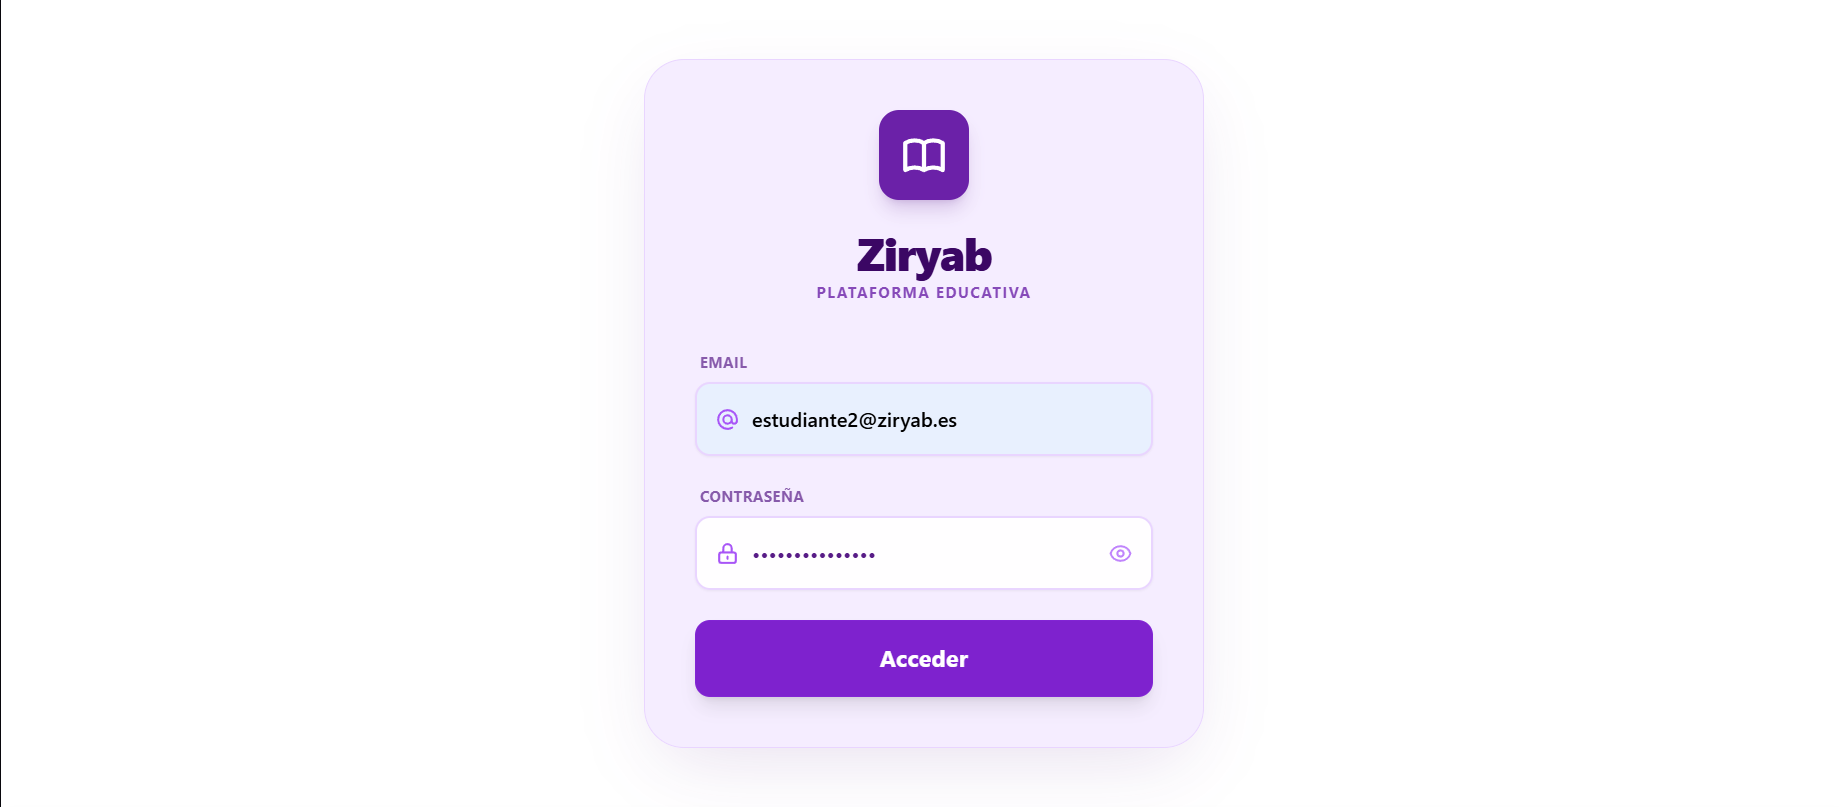
\includegraphics[keepaspectratio,alt={CAPTURA 1 --- Pantalla de login}]{../../assets/screenshots/manual-alumno/captura01-login.png}}
\caption{CAPTURA 1 --- Pantalla de login}
\end{figure}

\subsection{3.2 Introducir credenciales}\label{introducir-credenciales}

\begin{enumerate}
\def\labelenumi{\arabic{enumi}.}
\tightlist
\item
  Escribe tu \textbf{email} en el primer campo (icono de sobre).
\item
  Escribe tu \textbf{contraseña} en el segundo campo.
\item
  Opcional: pulsa el icono del ojo para \textbf{mostrar u ocultar} la
  contraseña.
\item
  Pulsa el botón principal para \textbf{acceder}.
\end{enumerate}

\subsection{3.3 Errores habituales en el
login}\label{errores-habituales-en-el-login}

\begin{itemize}
\tightlist
\item
  Si las credenciales son incorrectas, aparece un \textbf{mensaje de
  error en rojo} bajo el formulario.
\item
  Si el campo email no es válido, el formulario no enviará la petición.
\item
  Tras un login correcto, entrarás al \textbf{panel principal (Mi
  Espacio)}.
\end{itemize}

\begin{figure}
\centering
\pandocbounded{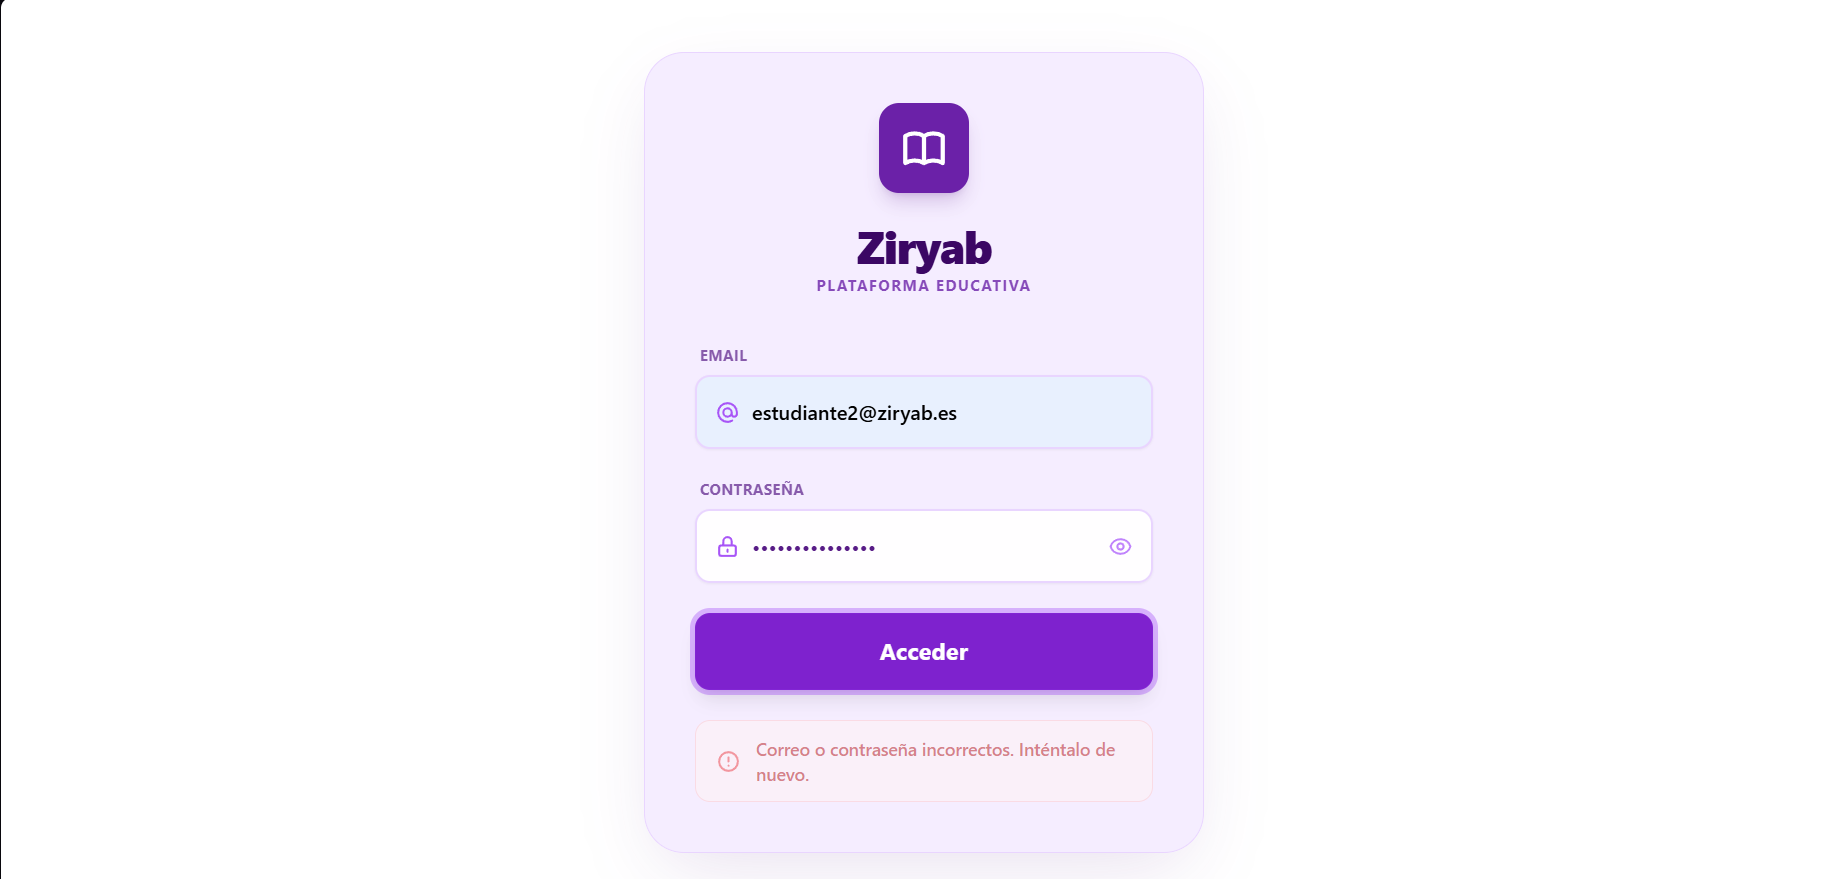
\includegraphics[keepaspectratio,alt={CAPTURA 2 --- Error de login}]{../../assets/screenshots/manual-alumno/captura02-error_login.png}}
\caption{CAPTURA 2 --- Error de login}
\end{figure}

\begin{center}\rule{0.5\linewidth}{0.5pt}\end{center}

\section{4. Interfaz general
(cabecera)}\label{interfaz-general-cabecera}

En todas las pantallas privadas verás una \textbf{cabecera morada} fija
con:

{\def\LTcaptype{none} % do not increment counter
\begin{longtable}[]{@{}
  >{\raggedright\arraybackslash}p{(\linewidth - 4\tabcolsep) * \real{0.3333}}
  >{\raggedright\arraybackslash}p{(\linewidth - 4\tabcolsep) * \real{0.3667}}
  >{\raggedright\arraybackslash}p{(\linewidth - 4\tabcolsep) * \real{0.3000}}@{}}
\toprule\noalign{}
\begin{minipage}[b]{\linewidth}\raggedright
Elemento
\end{minipage} & \begin{minipage}[b]{\linewidth}\raggedright
Ubicación
\end{minipage} & \begin{minipage}[b]{\linewidth}\raggedright
Función
\end{minipage} \\
\midrule\noalign{}
\endhead
\bottomrule\noalign{}
\endlastfoot
Selector de idioma & Izquierda & Cambia entre ES / EN / DE \\
Logotipo \textbf{Ziryab} & Centro & Al pulsar, vuelves al
\textbf{Dashboard} \\
Campana de notificaciones & Derecha & Abre el panel de notificaciones \\
Bloque de perfil (nombre + rol) & Derecha & Abre el menú de perfil \\
\end{longtable}
}

\begin{figure}
\centering
\pandocbounded{
\includegraphics[keepaspectratio,alt={CAPTURA 3 --- Cabecera de alumno}]{../../assets/screenshots/manual-alumno/captura03-cabecera.png}}
\caption{CAPTURA 3 --- Cabecera de alumno}
\end{figure}

\subsection{4.1 Notificaciones}\label{notificaciones}

\begin{enumerate}
\def\labelenumi{\arabic{enumi}.}
\tightlist
\item
  Pulsa la \textbf{campana}; se abre un panel lateral o desplegable.
\item
  Verás la lista de avisos (tareas nuevas, calificaciones, etc.).
\item
  Puedes \textbf{marcar todas como leídas} si la opción está disponible.
\item
  Al llegar una notificación en tiempo real, puede aparecer un
  \textbf{toast} (aviso flotante) en la parte inferior de la pantalla
  durante unos segundos.
\end{enumerate}

\begin{figure}
\centering
\pandocbounded{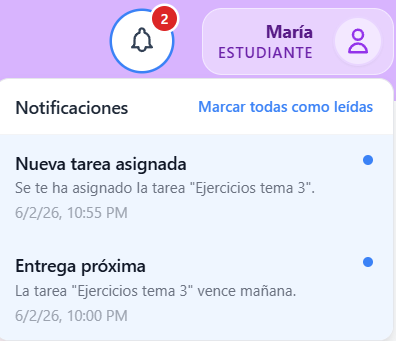
\includegraphics[keepaspectratio,alt={CAPTURA 4 --- Panel de notificaciones abierto}]{../../assets/screenshots/manual-alumno/captura04-notificaciones.png}}
\caption{CAPTURA 4 --- Panel de notificaciones abierto}
\end{figure}

\subsection{4.2 Menú de perfil y cierre de
sesión}\label{menuxfa-de-perfil-y-cierre-de-sesiuxf3n}

\begin{enumerate}
\def\labelenumi{\arabic{enumi}.}
\tightlist
\item
  Pulsa tu \textbf{nombre y avatar} en la cabecera.
\item
  Se abre un modal con tu nombre, rol y el botón \textbf{Cerrar sesión}.
\item
  Confirma el cierre; volverás a la pantalla de login.
\end{enumerate}

\begin{figure}
\centering
\pandocbounded{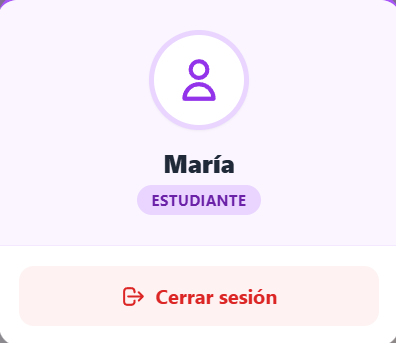
\includegraphics[keepaspectratio,alt={CAPTURA 5 --- Modal de perfil con botón Cerrar sesión}]{../../assets/screenshots/manual-alumno/captura05-modal_perfil.png}}
\caption{CAPTURA 5 --- Modal de perfil con botón Cerrar sesión}
\end{figure}

\subsection{4.3 Botón «Volver»}\label{botuxf3n-volver}

En la mayoría de pantallas secundarias aparece el componente
\textbf{Volver} (flecha atrás), que te lleva a la pantalla anterior en
el historial de navegación.

\begin{center}\rule{0.5\linewidth}{0.5pt}\end{center}

\section{5. Panel principal --- «Mi Espacio»
(Dashboard)}\label{panel-principal-mi-espacio-dashboard}

Tras iniciar sesión accedes a \textbf{Mi Espacio}, con el mensaje
\emph{«¿Qué te gustaría hacer hoy?»} y \textbf{dos tarjetas grandes}:

{\def\LTcaptype{none} % do not increment counter
\begin{longtable}[]{@{}
  >{\raggedright\arraybackslash}p{(\linewidth - 4\tabcolsep) * \real{0.2903}}
  >{\raggedright\arraybackslash}p{(\linewidth - 4\tabcolsep) * \real{0.4194}}
  >{\raggedright\arraybackslash}p{(\linewidth - 4\tabcolsep) * \real{0.2903}}@{}}
\toprule\noalign{}
\begin{minipage}[b]{\linewidth}\raggedright
Tarjeta
\end{minipage} & \begin{minipage}[b]{\linewidth}\raggedright
Descripción
\end{minipage} & \begin{minipage}[b]{\linewidth}\raggedright
Destino
\end{minipage} \\
\midrule\noalign{}
\endhead
\bottomrule\noalign{}
\endlastfoot
\textbf{Clases} & Accede a tus asignaturas matriculadas &
\texttt{/clases} \\
\textbf{Gestión} & Expediente, horario, calendario, avisos y notas &
\texttt{/gestion} \\
\end{longtable}
}

\begin{enumerate}
\def\labelenumi{\arabic{enumi}.}
\tightlist
\item
  Haz clic en la tarjeta deseada (también al pasar el ratón verás la
  etiqueta \textbf{Acceder}).
\end{enumerate}

\begin{figure}
\centering
\pandocbounded{
\includegraphics[keepaspectratio,alt={CAPTURA 6 --- Dashboard «Mi Espacio»}]{../../assets/screenshots/manual-alumno/captura06-dashboard.png}}
\caption{CAPTURA 6 --- Dashboard «Mi Espacio»}
\end{figure}

\begin{center}\rule{0.5\linewidth}{0.5pt}\end{center}

\section{6. Mis asignaturas (Clases)}\label{mis-asignaturas-clases}

\subsection{6.1 Listado de asignaturas}\label{listado-de-asignaturas}

Ruta: \textbf{Dashboard → Clases} (\texttt{/clases}).

\begin{itemize}
\tightlist
\item
  Verás una \textbf{rejilla de tarjetas}, una por cada asignatura en la
  que estás matriculado.
\item
  Cada tarjeta muestra, entre otros datos: \textbf{nombre de la
  asignatura}, \textbf{ciclo/curso}, \textbf{grupo} y \textbf{profesor}
  (cuando esté disponible).
\item
  Mientras carga, aparece el mensaje \emph{«Cargando tus clases\ldots»}.
\item
  Si no tienes matrículas, verás \emph{«No estás matriculado en ninguna
  asignatura»}.
\end{itemize}

\begin{figure}
\centering
\pandocbounded{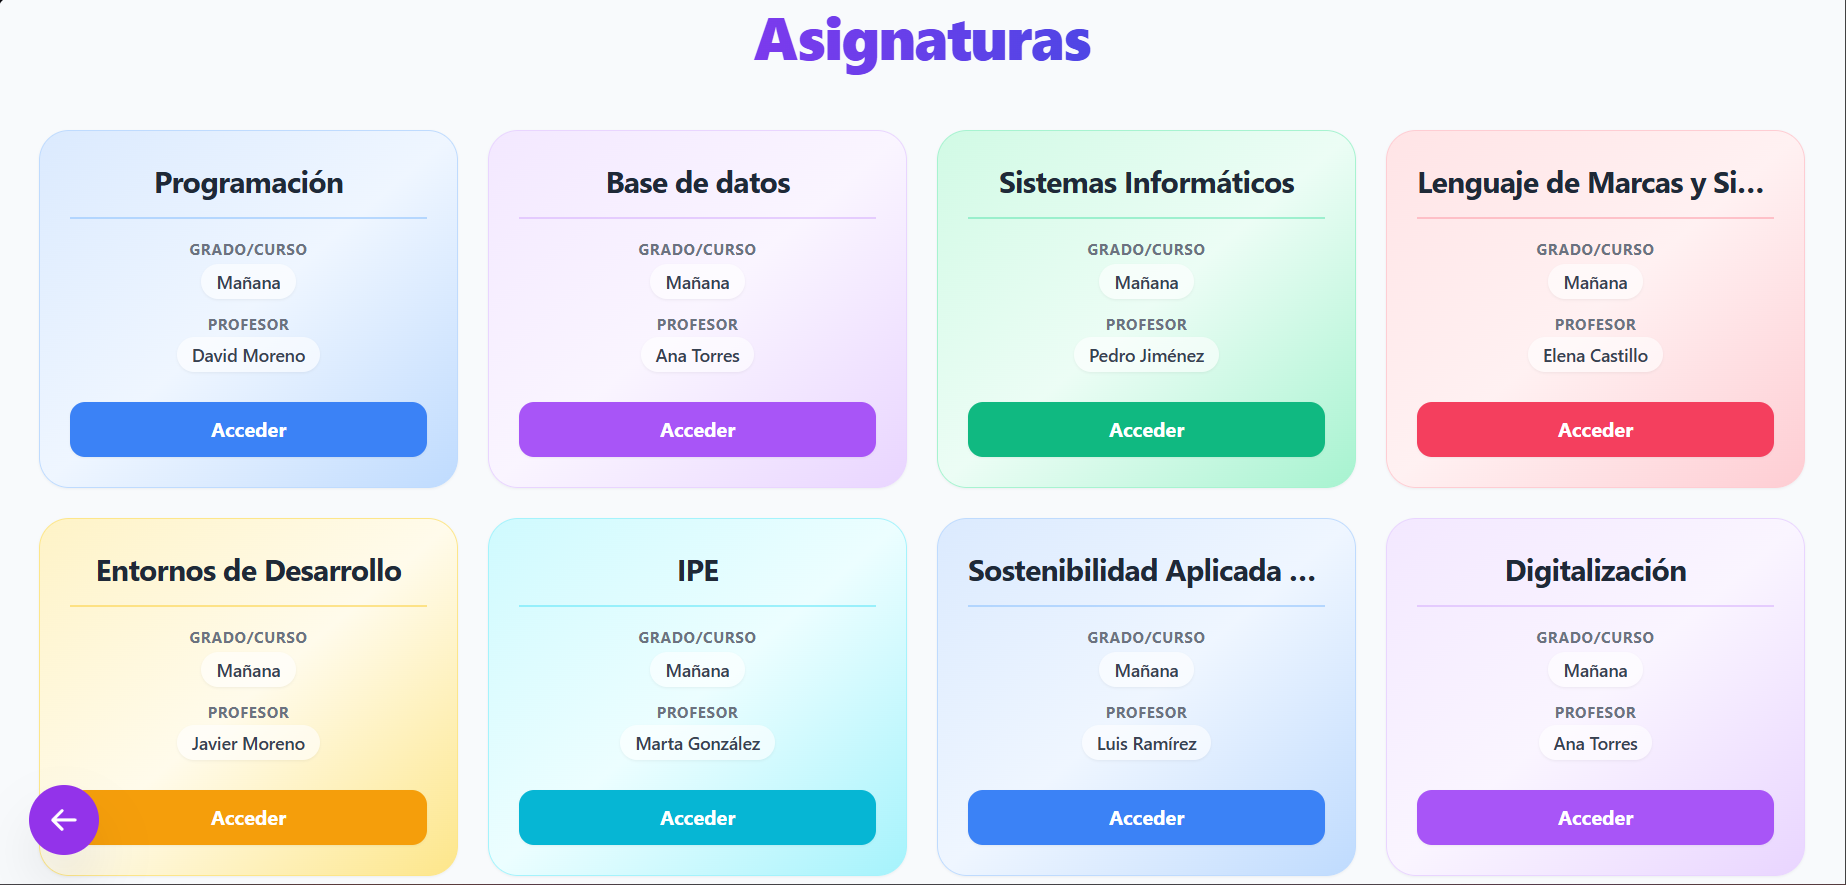
\includegraphics[keepaspectratio,alt={CAPTURA 7 --- Listado de asignaturas del alumno}]{../../assets/screenshots/manual-alumno/captura07-asignaturas.png}}
\caption{CAPTURA 7 --- Listado de asignaturas del alumno}
\end{figure}

\subsection{6.2 Entrar al temario de una
asignatura}\label{entrar-al-temario-de-una-asignatura}

\begin{enumerate}
\def\labelenumi{\arabic{enumi}.}
\tightlist
\item
  En la tarjeta de la asignatura, pulsa la acción principal (abrir /
  acceder al temario).
\item
  Irás a \textbf{Temario} (\texttt{/temario/:claseId}) con el material y
  las tareas de esa asignatura.
\end{enumerate}

\begin{center}\rule{0.5\linewidth}{0.5pt}\end{center}

\section{7. Temario y listado de
tareas}\label{temario-y-listado-de-tareas}

\subsection{7.1 Estructura del temario}\label{estructura-del-temario}

El temario organiza el contenido en \textbf{bloques desplegables} por
tipo:

\begin{itemize}
\tightlist
\item
  Material teórico y documentos\\
\item
  Exámenes y pruebas\\
\item
  Proyectos evaluables\\
\item
  Ejercicios prácticos\\
\item
  Deberes generales
\end{itemize}

\begin{enumerate}
\def\labelenumi{\arabic{enumi}.}
\tightlist
\item
  Pulsa la cabecera de un bloque para \textbf{expandirlo o contraerlo}.
\item
  Dentro verás las \textbf{tareas} con título, fecha límite y
  \textbf{estado}.
\end{enumerate}

\begin{figure}
\centering
\pandocbounded{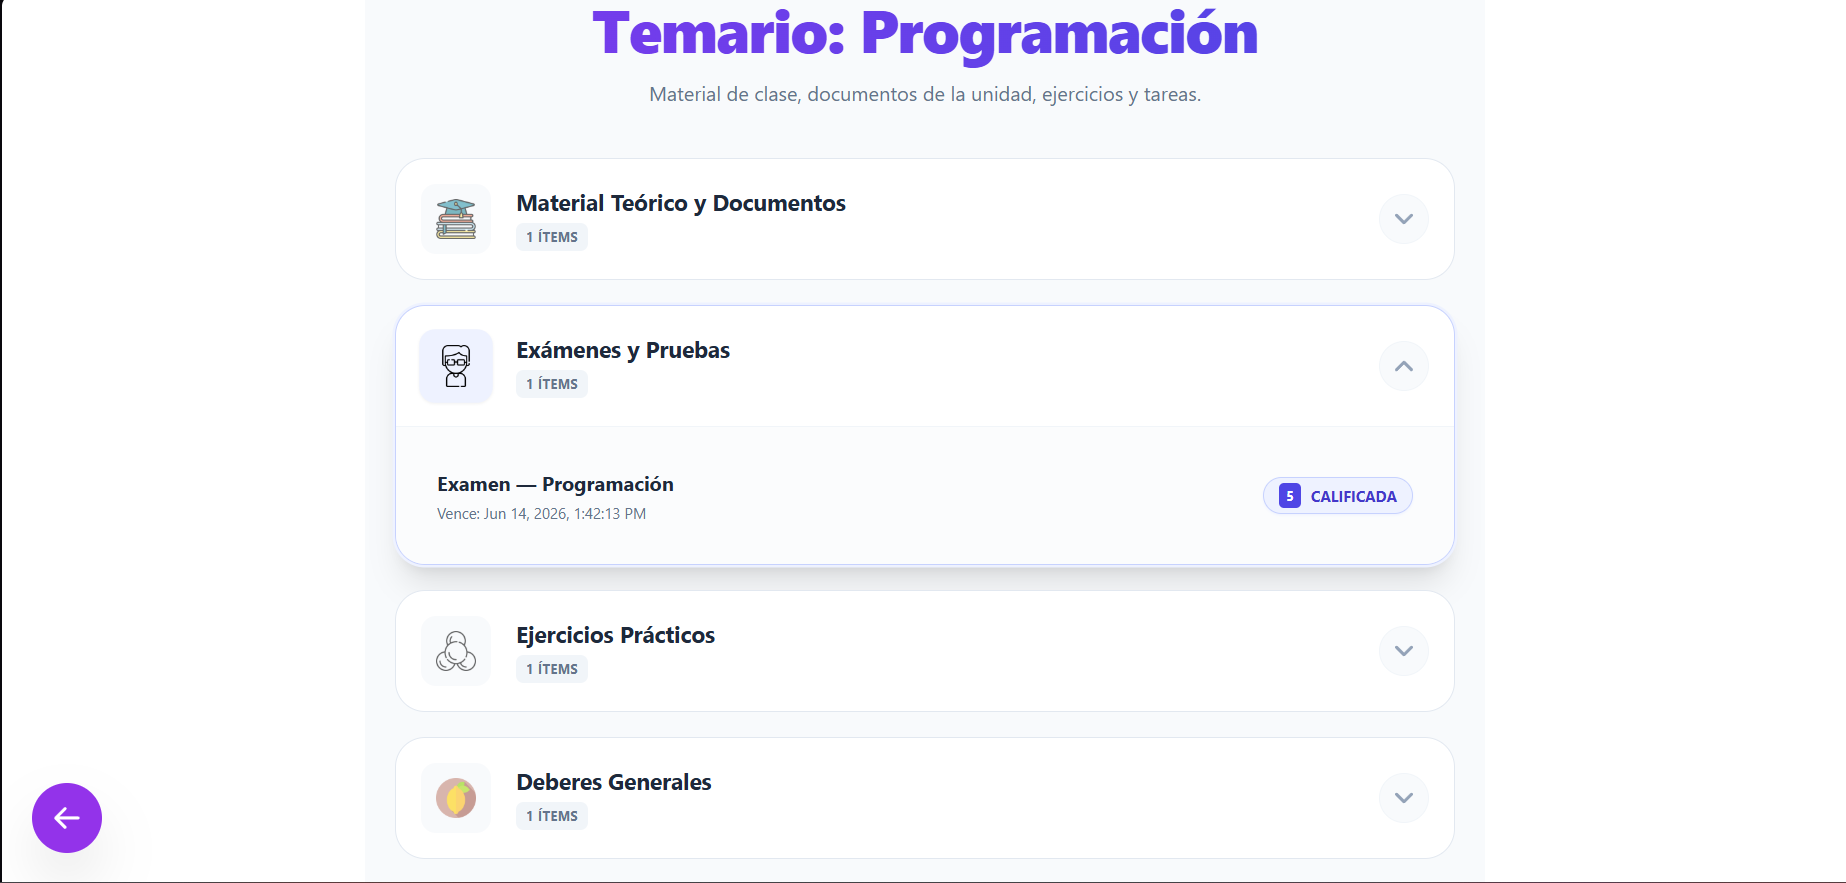
\includegraphics[keepaspectratio,alt={CAPTURA 8 --- Temario con bloques y tareas}]{../../assets/screenshots/manual-alumno/captura08-temario.png}}
\caption{CAPTURA 8 --- Temario con bloques y tareas}
\end{figure}

\subsection{7.2 Estados de una tarea (en el
listado)}\label{estados-de-una-tarea-en-el-listado}

{\def\LTcaptype{none} % do not increment counter
\begin{longtable}[]{@{}
  >{\raggedright\arraybackslash}p{(\linewidth - 2\tabcolsep) * \real{0.3810}}
  >{\raggedright\arraybackslash}p{(\linewidth - 2\tabcolsep) * \real{0.6190}}@{}}
\toprule\noalign{}
\begin{minipage}[b]{\linewidth}\raggedright
Estado
\end{minipage} & \begin{minipage}[b]{\linewidth}\raggedright
Significado
\end{minipage} \\
\midrule\noalign{}
\endhead
\bottomrule\noalign{}
\endlastfoot
\textbf{PENDIENTE} & Aún no has entregado (puede estar dentro o fuera de
plazo) \\
\textbf{ENTREGADA} & Has enviado tu trabajo; pendiente de corrección \\
\textbf{CALIFICADA} & El profesor ha puesto nota (se muestra la
puntuación) \\
\textbf{VENCIDA} & Plazo pasado sin entrega válida \\
\end{longtable}
}

\subsection{7.3 Abrir el detalle de una
tarea}\label{abrir-el-detalle-de-una-tarea}

\begin{enumerate}
\def\labelenumi{\arabic{enumi}.}
\tightlist
\item
  Pulsa sobre la fila de la tarea.
\item
  Se abre la pantalla de \textbf{detalle de tarea}
  (\texttt{/tarea/:id}).
\end{enumerate}

\begin{center}\rule{0.5\linewidth}{0.5pt}\end{center}

\section{8. Detalle de tarea: consulta, entrega y
nota}\label{detalle-de-tarea-consulta-entrega-y-nota}

\subsection{8.1 Información de la
tarea}\label{informaciuxf3n-de-la-tarea}

En la parte superior verás:

\begin{itemize}
\tightlist
\item
  \textbf{Título} y \textbf{estado} (badge de color)
\item
  \textbf{Fecha límite} de entrega
\item
  \textbf{Tipo} de tarea (deberes, práctica, examen, etc.)
\item
  \textbf{Descripción} del profesor
\item
  \textbf{Material de consulta}: enlace para ver o descargar el archivo
  adjunto del profesor (si existe)
\end{itemize}

\begin{figure}
\centering
\pandocbounded{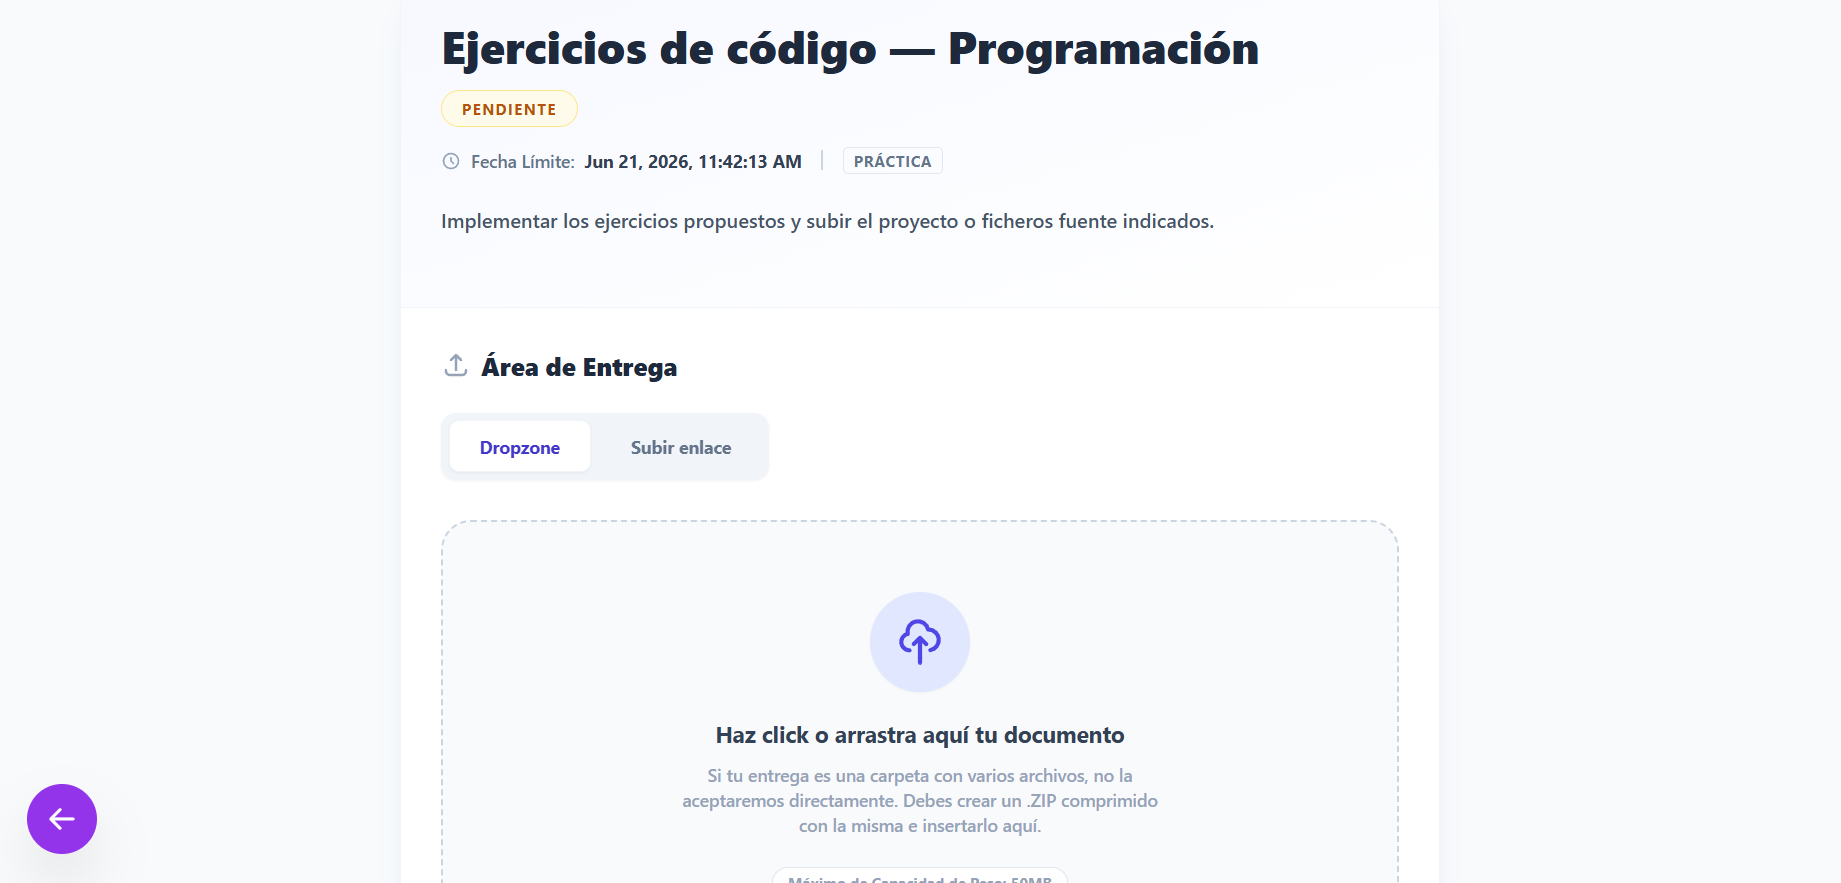
\includegraphics[keepaspectratio,alt={CAPTURA 9 --- Detalle de tarea}]{../../assets/screenshots/manual-alumno/captura09-detalle_tarea.png}}
\caption{CAPTURA 9 --- Detalle de tarea}
\end{figure}

\subsection{8.2 Si la tarea ya está
calificada}\label{si-la-tarea-ya-estuxe1-calificada}

Aparece la sección \textbf{Evaluación del profesor} con:

\begin{itemize}
\tightlist
\item
  \textbf{Nota final} (0--10)
\item
  \textbf{Comentarios} del profesor (si los hubo)
\end{itemize}

\begin{figure}
\centering
\pandocbounded{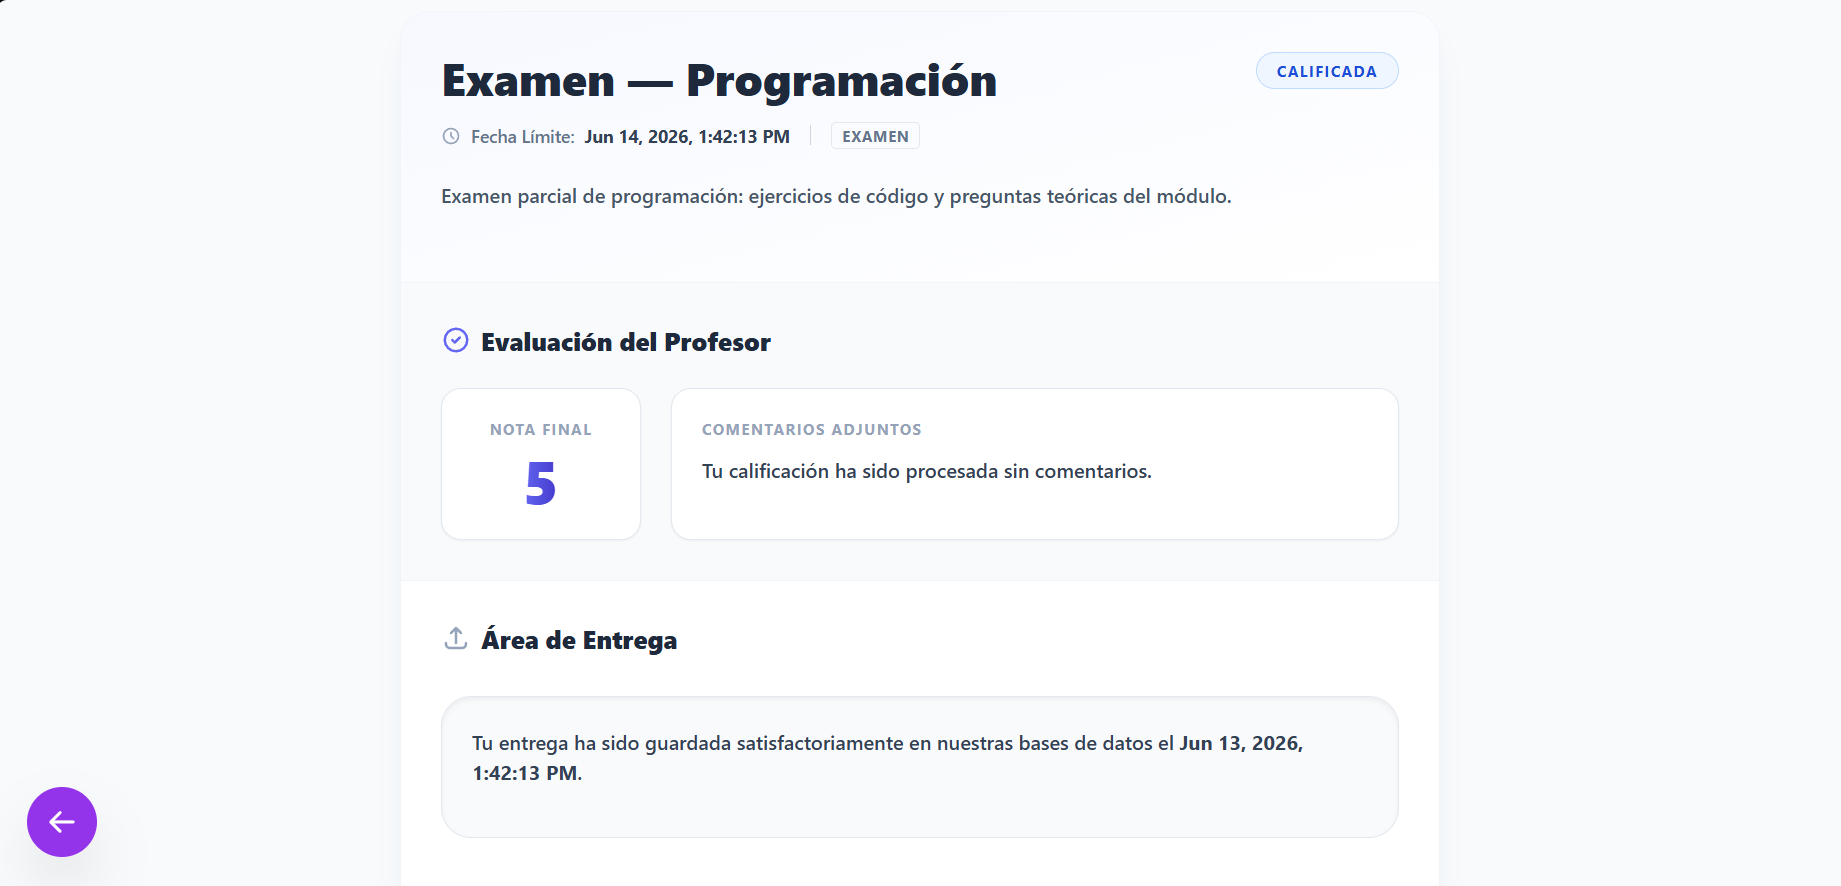
\includegraphics[keepaspectratio,alt={CAPTURA 10 --- Tarea entregada / evaluación del profesor}]{../../assets/screenshots/manual-alumno/captura10-tarea_entregada.png}}
\caption{CAPTURA 10 --- Tarea entregada / evaluación del profesor}
\end{figure}

\subsection{8.3 Entregar una tarea
(pendiente)}\label{entregar-una-tarea-pendiente}

En el \textbf{Área de entrega} puedes elegir dos modos:

\subsubsection{Modo A --- Subir archivo
(Dropzone)}\label{modo-a-subir-archivo-dropzone}

\begin{enumerate}
\def\labelenumi{\arabic{enumi}.}
\tightlist
\item
  Selecciona la pestaña de subida de archivo.
\item
  \textbf{Arrastra} un archivo a la zona punteada \textbf{o} haz clic
  para elegirlo en el explorador.
\item
  Formatos habituales: documentos, imágenes, ZIP (si son varios
  archivos, \textbf{comprime en .ZIP}).
\item
  Tamaño máximo indicado en pantalla: \textbf{50 MB}.
\item
  Tras seleccionar el archivo, revisa el nombre y pulsa
  \textbf{Confirmar envío al servidor}.
\end{enumerate}

\begin{figure}
\centering
\pandocbounded{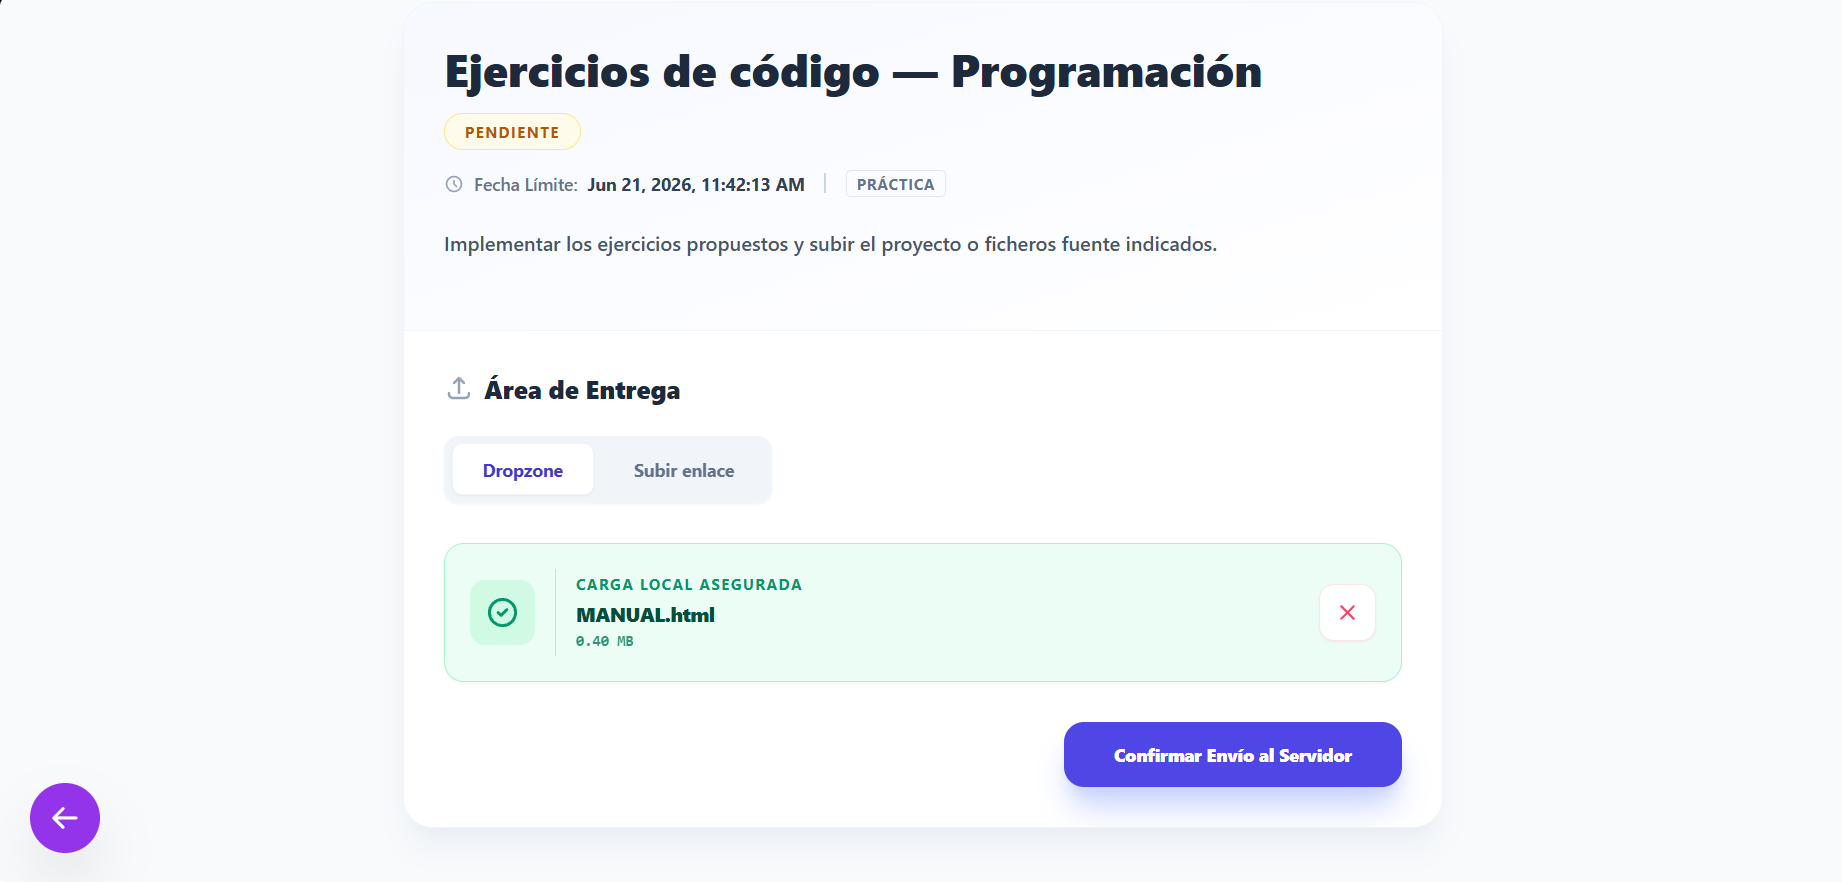
\includegraphics[keepaspectratio,alt={CAPTURA 11 --- Zona de arrastre con archivo seleccionado}]{../../assets/screenshots/manual-alumno/captura11-tarea_subida.png}}
\caption{CAPTURA 11 --- Zona de arrastre con archivo seleccionado}
\end{figure}

\subsubsection{Modo B --- Enlace URL}\label{modo-b-enlace-url}

\begin{enumerate}
\def\labelenumi{\arabic{enumi}.}
\tightlist
\item
  Cambia a la pestaña \textbf{Subir enlace}.
\item
  Introduce una URL válida (\texttt{http://} o \texttt{https://}), por
  ejemplo un Google Docs.
\item
  Pulsa \textbf{Confirmar envío al servidor}.
\end{enumerate}

\begin{figure}
\centering
\pandocbounded{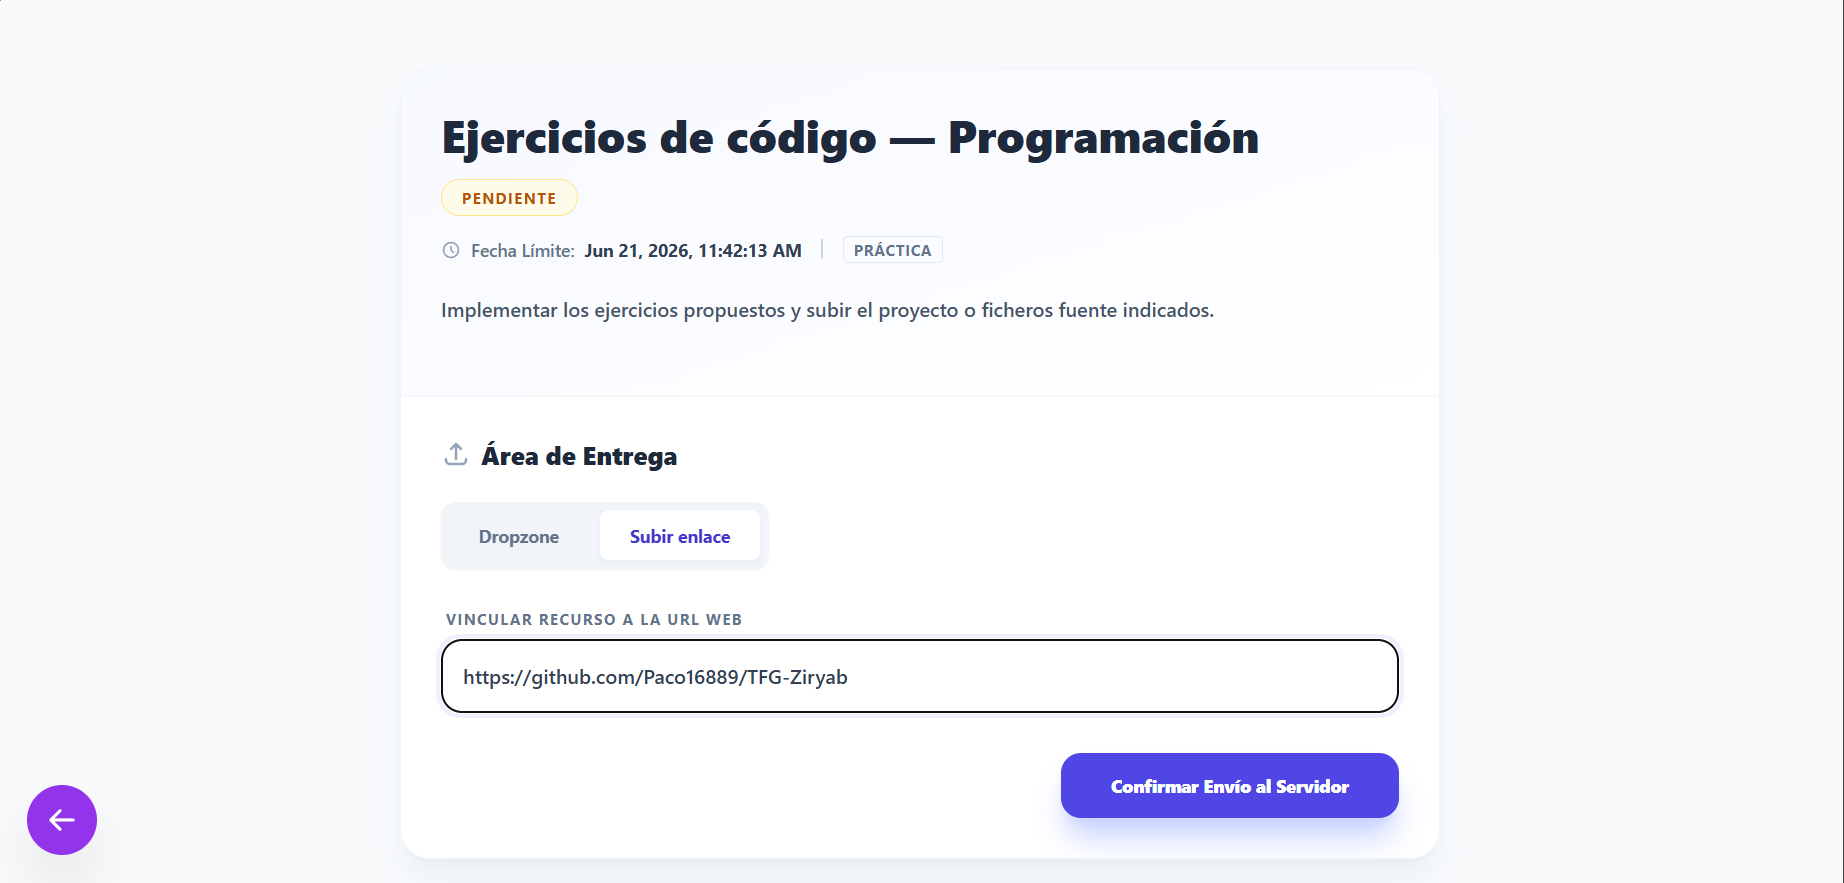
\includegraphics[keepaspectratio,alt={CAPTURA 12 --- Pestaña de enlace con URL rellenada}]{../../assets/screenshots/manual-alumno/captura12-enlace_entregado.png}}
\caption{CAPTURA 12 --- Pestaña de enlace con URL rellenada}
\end{figure}

\subsection{8.4 Avisos importantes al
entregar}\label{avisos-importantes-al-entregar}

\begin{itemize}
\tightlist
\item
  Si el plazo ha pasado pero el profesor \textbf{permite entrega
  tardía}, tu entrega puede quedar como \textbf{Retraso (LATE)}.
\item
  Si el plazo ha pasado y \textbf{no} se permiten entregas tardías,
  verás un aviso y \textbf{no podrás enviar}.
\item
  Tras un envío correcto aparece mensaje verde de confirmación.
\end{itemize}

\subsection{8.5 Modificar o borrar una
entrega}\label{modificar-o-borrar-una-entrega}

\begin{itemize}
\tightlist
\item
  Si ya entregaste y \textbf{aún no está calificada}, puedes usar
  \textbf{Borrar entrega} y volver a subir.
\item
  Si ya está \textbf{calificada}, no podrás eliminar la entrega desde
  esta pantalla.
\end{itemize}

\subsection{8.6 Errores frecuentes en la
entrega}\label{errores-frecuentes-en-la-entrega}

{\def\LTcaptype{none} % do not increment counter
\begin{longtable}[]{@{}ll@{}}
\toprule\noalign{}
Mensaje / situación & Qué hacer \\
\midrule\noalign{}
\endhead
\bottomrule\noalign{}
\endlastfoot
Carpeta no permitida & Comprime la carpeta en un archivo
\textbf{.ZIP} \\
Archivo demasiado grande & Reduce el tamaño por debajo de 50 MB \\
URL inválida & Comprueba que empiece por http:// o https:// \\
Error de servidor & Reintenta; si persiste, contacta con el profesor \\
\end{longtable}
}

\begin{center}\rule{0.5\linewidth}{0.5pt}\end{center}

\section{9. Gestión académica (menú
central)}\label{gestiuxf3n-acaduxe9mica-menuxfa-central}

Ruta: \textbf{Dashboard → Gestión} (\texttt{/gestion}).

Pantalla \textbf{Gestión académica} con acceso a cinco áreas:

{\def\LTcaptype{none} % do not increment counter
\begin{longtable}[]{@{}ll@{}}
\toprule\noalign{}
Tarjeta & Función \\
\midrule\noalign{}
\endhead
\bottomrule\noalign{}
\endlastfoot
\textbf{Ficha Usuario} & Historial de faltas y justificantes \\
\textbf{Horario} & Horario semanal de clases \\
\textbf{Calendario} & Calendario del centro (vista embebida) \\
\textbf{Tablón} & Anuncios / incidencias publicadas \\
\textbf{Evaluaciones} & Tus notas por trimestre \\
\end{longtable}
}

\begin{figure}
\centering
\pandocbounded{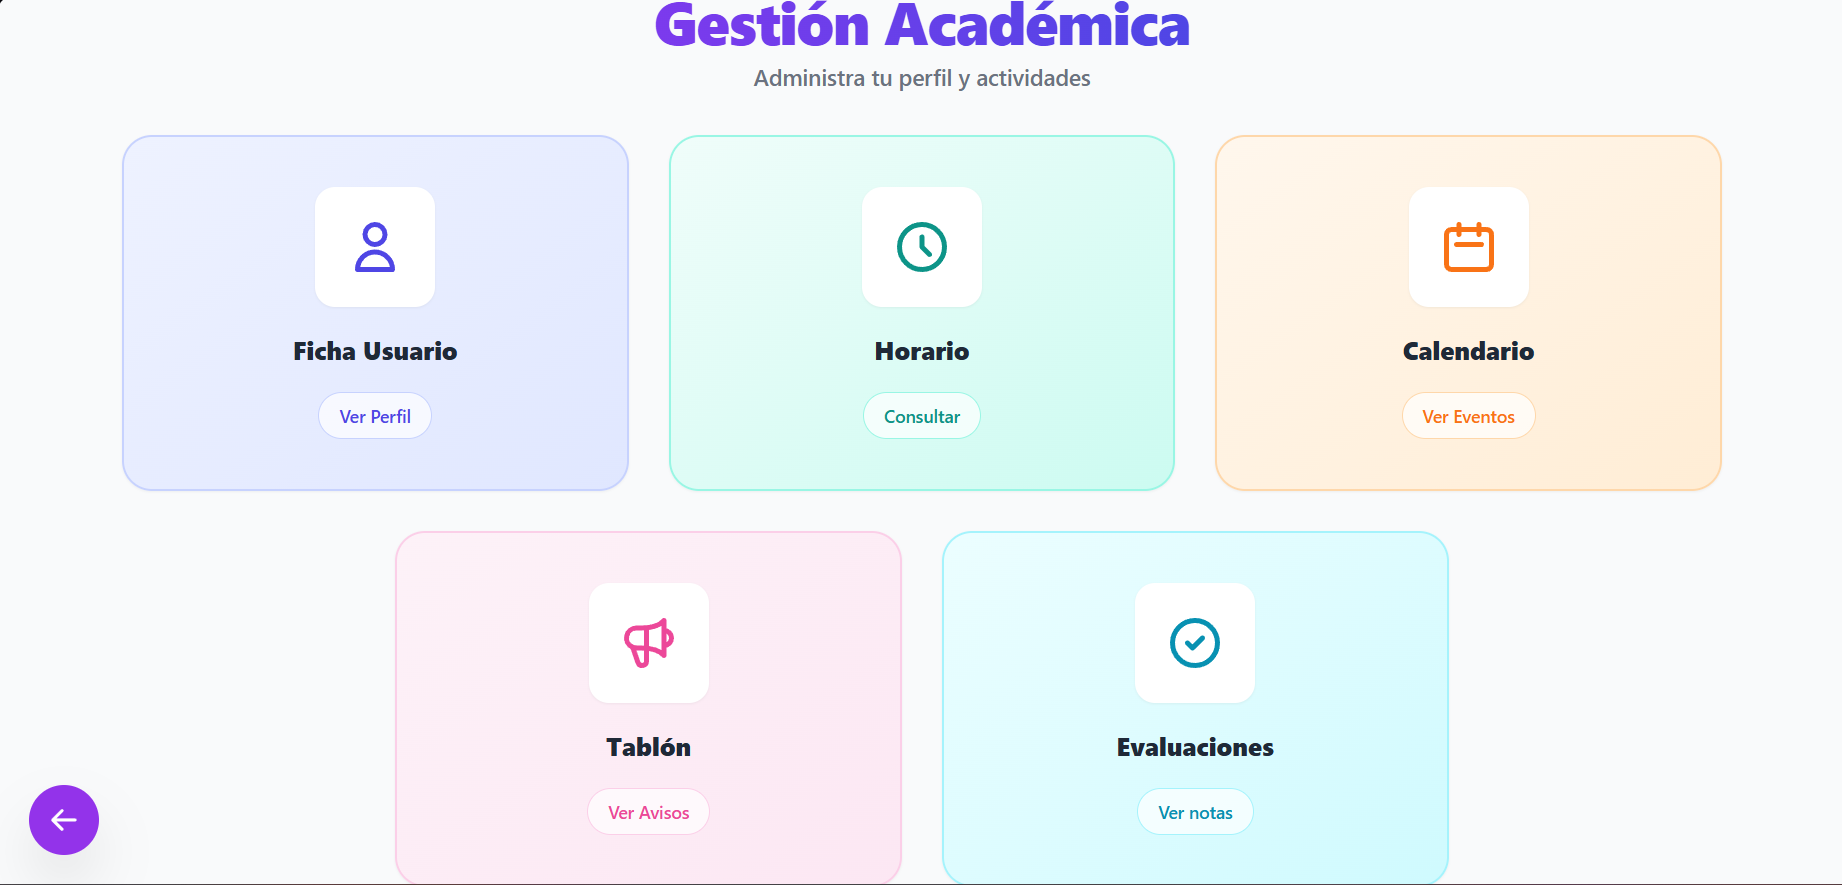
\includegraphics[keepaspectratio,alt={CAPTURA 13 --- Pantalla Gestión académica}]{../../assets/screenshots/manual-alumno/captura13-pantalla_gestion.png}}
\caption{CAPTURA 13 --- Pantalla Gestión académica}
\end{figure}

\begin{center}\rule{0.5\linewidth}{0.5pt}\end{center}

\section{10. Ficha de usuario y
asistencia}\label{ficha-de-usuario-y-asistencia}

Ruta: \textbf{Gestión → Ficha Usuario} (\texttt{/ficha-usuario}).

\subsection{10.1 Consultar faltas}\label{consultar-faltas}

\begin{itemize}
\tightlist
\item
  Listado de \textbf{faltas y retrasos} registrados por sesión.
\item
  Cada fila muestra: \textbf{asignatura}, \textbf{fecha}, \textbf{hora},
  \textbf{estado de asistencia} y \textbf{estado del justificante}.
\item
  Si no tienes faltas, verás un mensaje positivo indicando que no hay
  registros.
\end{itemize}

Estados de asistencia:

{\def\LTcaptype{none} % do not increment counter
\begin{longtable}[]{@{}ll@{}}
\toprule\noalign{}
Etiqueta & Significado \\
\midrule\noalign{}
\endhead
\bottomrule\noalign{}
\endlastfoot
FALTA & Ausencia \\
RETRASO & Llegada tarde \\
JUSTIFICADA & Falta excusada oficialmente \\
\end{longtable}
}

\begin{figure}
\centering
\pandocbounded{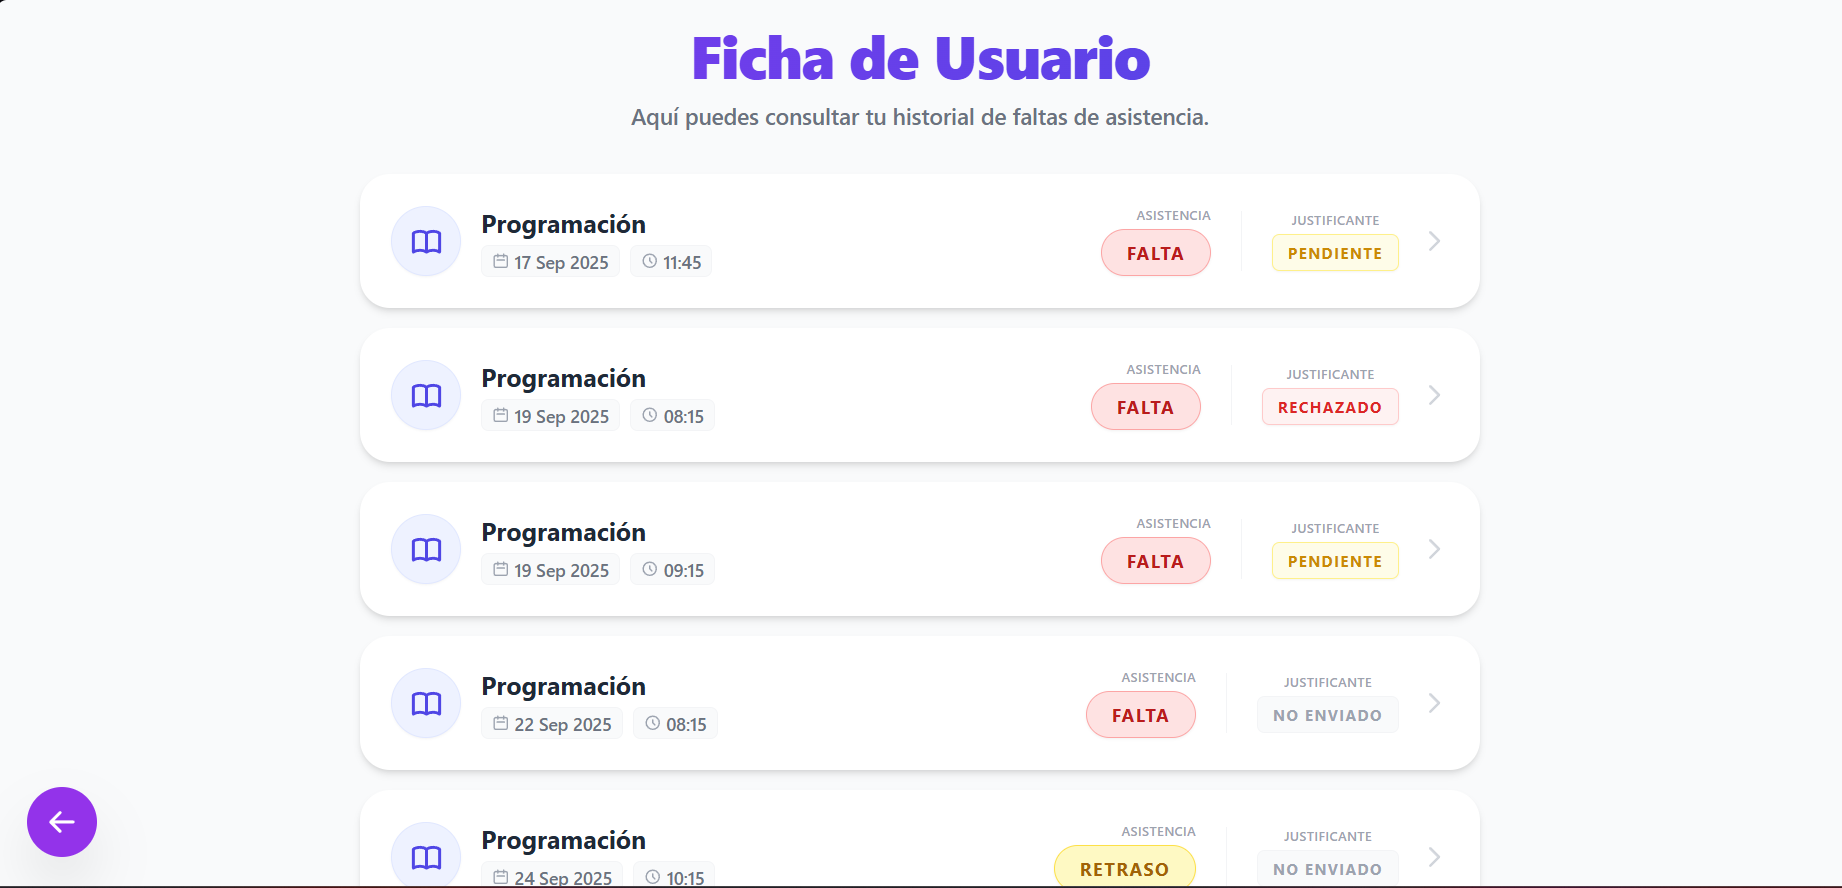
\includegraphics[keepaspectratio,alt={CAPTURA 14 --- Listado de faltas}]{../../assets/screenshots/manual-alumno/captura14-ficha_usuario.png}}
\caption{CAPTURA 14 --- Listado de faltas}
\end{figure}

\subsection{10.2 Justificar una falta}\label{justificar-una-falta}

\begin{enumerate}
\def\labelenumi{\arabic{enumi}.}
\tightlist
\item
  Pulsa sobre una falta que \textbf{no} esté ya justificada (filas
  interactivas).
\item
  Se abre el modal \textbf{Justificar falta}.
\item
  Selecciona un documento: \textbf{PNG, JPG o PDF}, máximo \textbf{1
  MB}.
\item
  Pulsa \textbf{Subir justificante}.
\item
  El estado pasará a \textbf{PENDIENTE} hasta que el profesor lo revise.
\end{enumerate}

\begin{figure}
\centering
\pandocbounded{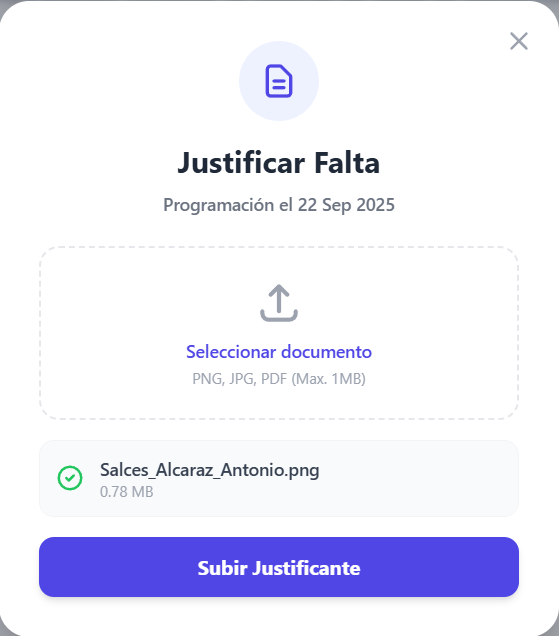
\includegraphics[keepaspectratio,alt={CAPTURA 15 --- Modal de justificación}]{../../assets/screenshots/manual-alumno/captura15-modal_justificar_falta.png}}
\caption{CAPTURA 15 --- Modal de justificación}
\end{figure}

\begin{figure}
\centering
\pandocbounded{
\includegraphics[keepaspectratio,alt={CAPTURA 16 --- Falta con justificante PENDIENTE}]{../../assets/screenshots/manual-alumno/captura16-justificacion_pendiente.png}}
\caption{CAPTURA 16 --- Falta con justificante PENDIENTE}
\end{figure}

Estados del justificante: \textbf{NO ENVIADO}, \textbf{PENDIENTE},
\textbf{ACEPTADO}, \textbf{RECHAZADO}.

\begin{center}\rule{0.5\linewidth}{0.5pt}\end{center}

\section{11. Horario semanal}\label{horario-semanal}

Ruta: \textbf{Gestión → Horario} (\texttt{/horario-alumno}).

\begin{itemize}
\tightlist
\item
  Vista en \textbf{columnas por día de la semana} (lunes a viernes o
  según configuración del centro).
\item
  En cada día aparecen las franjas con \textbf{hora inicio--fin} y
  \textbf{nombre de la asignatura}.
\item
  Si un día no tienes clase, verás un mensaje de día sin clases.
\end{itemize}

\begin{figure}
\centering
\pandocbounded{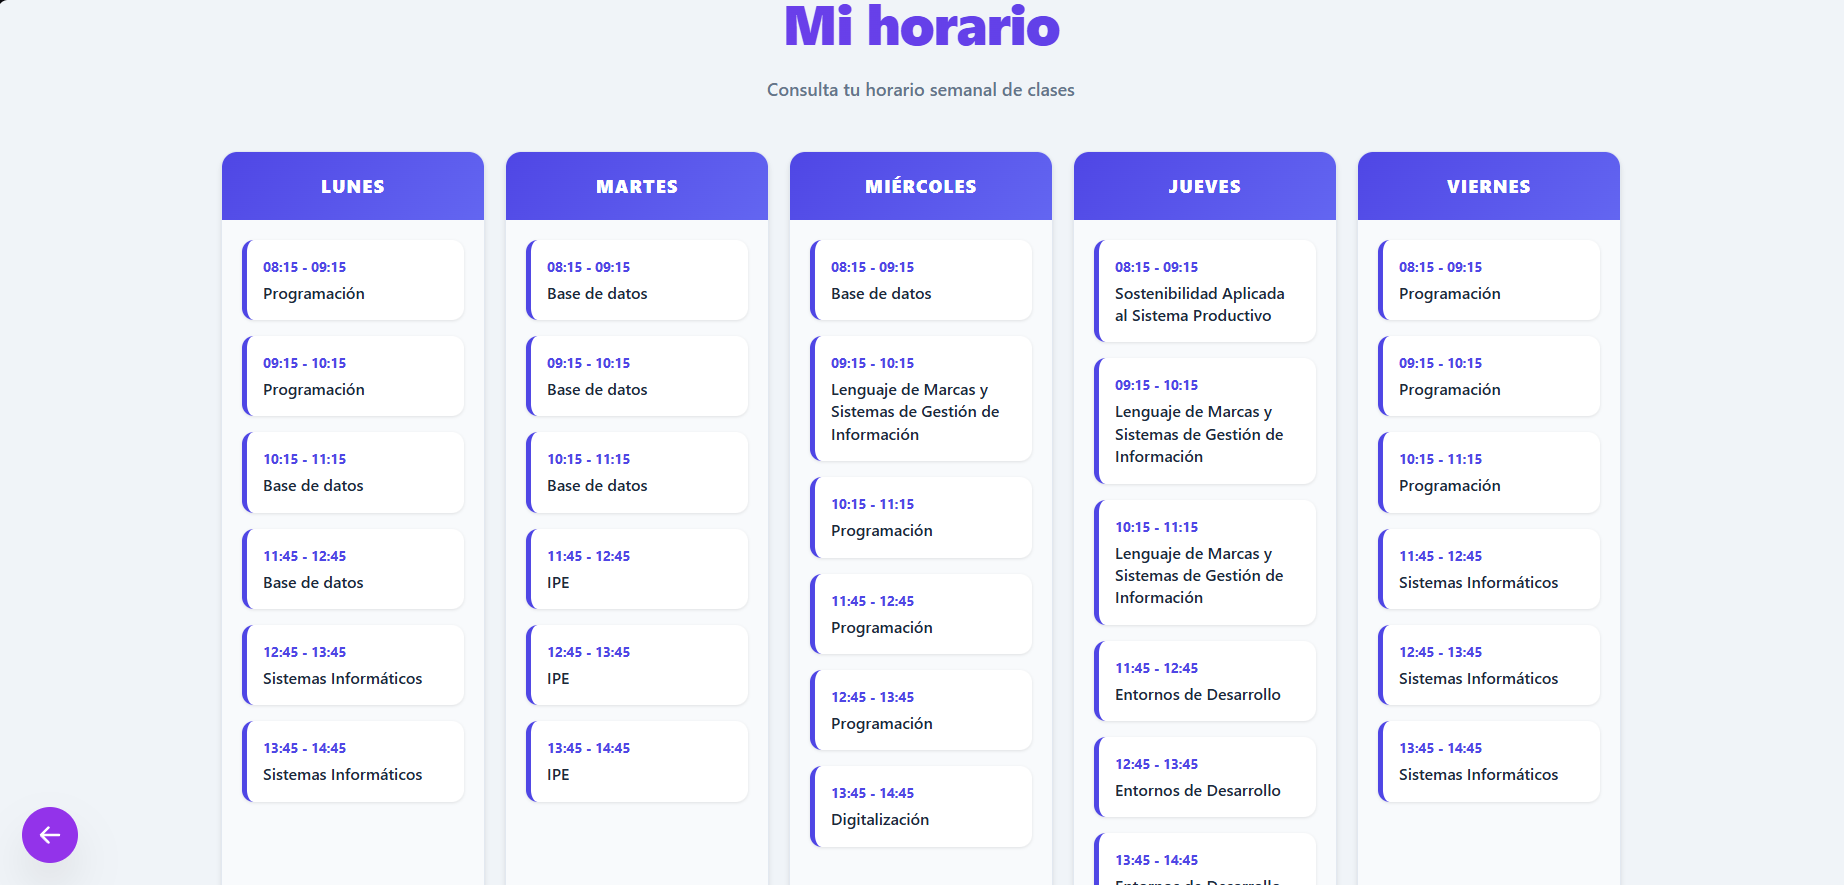
\includegraphics[keepaspectratio,alt={CAPTURA 17 --- Horario semanal del alumno}]{../../assets/screenshots/manual-alumno/captura17-horario.png}}
\caption{CAPTURA 17 --- Horario semanal del alumno}
\end{figure}

\begin{center}\rule{0.5\linewidth}{0.5pt}\end{center}

\section{12. Calendario}\label{calendario}

Ruta: \textbf{Gestión → Calendario} (\texttt{/calendario}).

\begin{itemize}
\tightlist
\item
  Muestra un \textbf{calendario embebido} (iframe) con eventos del
  centro.
\item
  Desplázate y navega dentro del calendario como en la herramienta
  externa configurada.
\end{itemize}

\begin{figure}
\centering
\pandocbounded{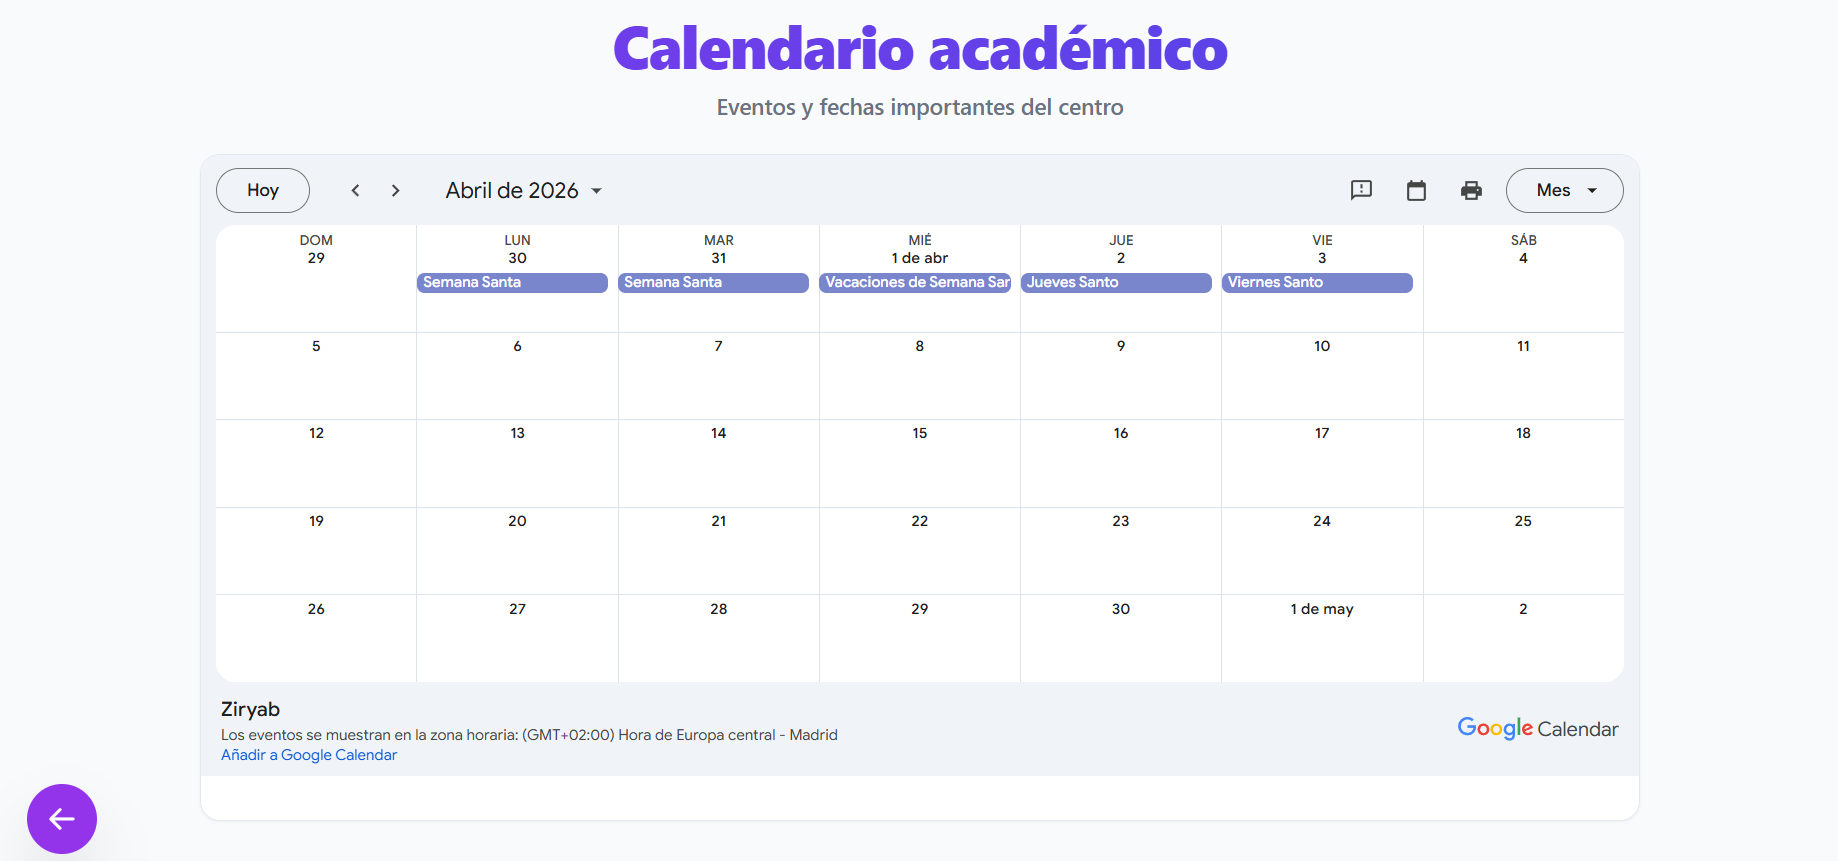
\includegraphics[keepaspectratio,alt={CAPTURA 18 --- Pantalla Calendario}]{../../assets/screenshots/manual-alumno/captura18-calendario.png}}
\caption{CAPTURA 18 --- Pantalla Calendario}
\end{figure}

\begin{center}\rule{0.5\linewidth}{0.5pt}\end{center}

\section{13. Tablón de anuncios}\label{tabluxf3n-de-anuncios}

Ruta: \textbf{Gestión → Tablón} (\texttt{/issues}).

\begin{itemize}
\tightlist
\item
  Listado de \textbf{anuncios} publicados para la comunidad educativa.
\item
  Consulta título, contenido y fecha de cada aviso (según diseño de la
  lista).
\end{itemize}

\begin{figure}
\centering
\pandocbounded{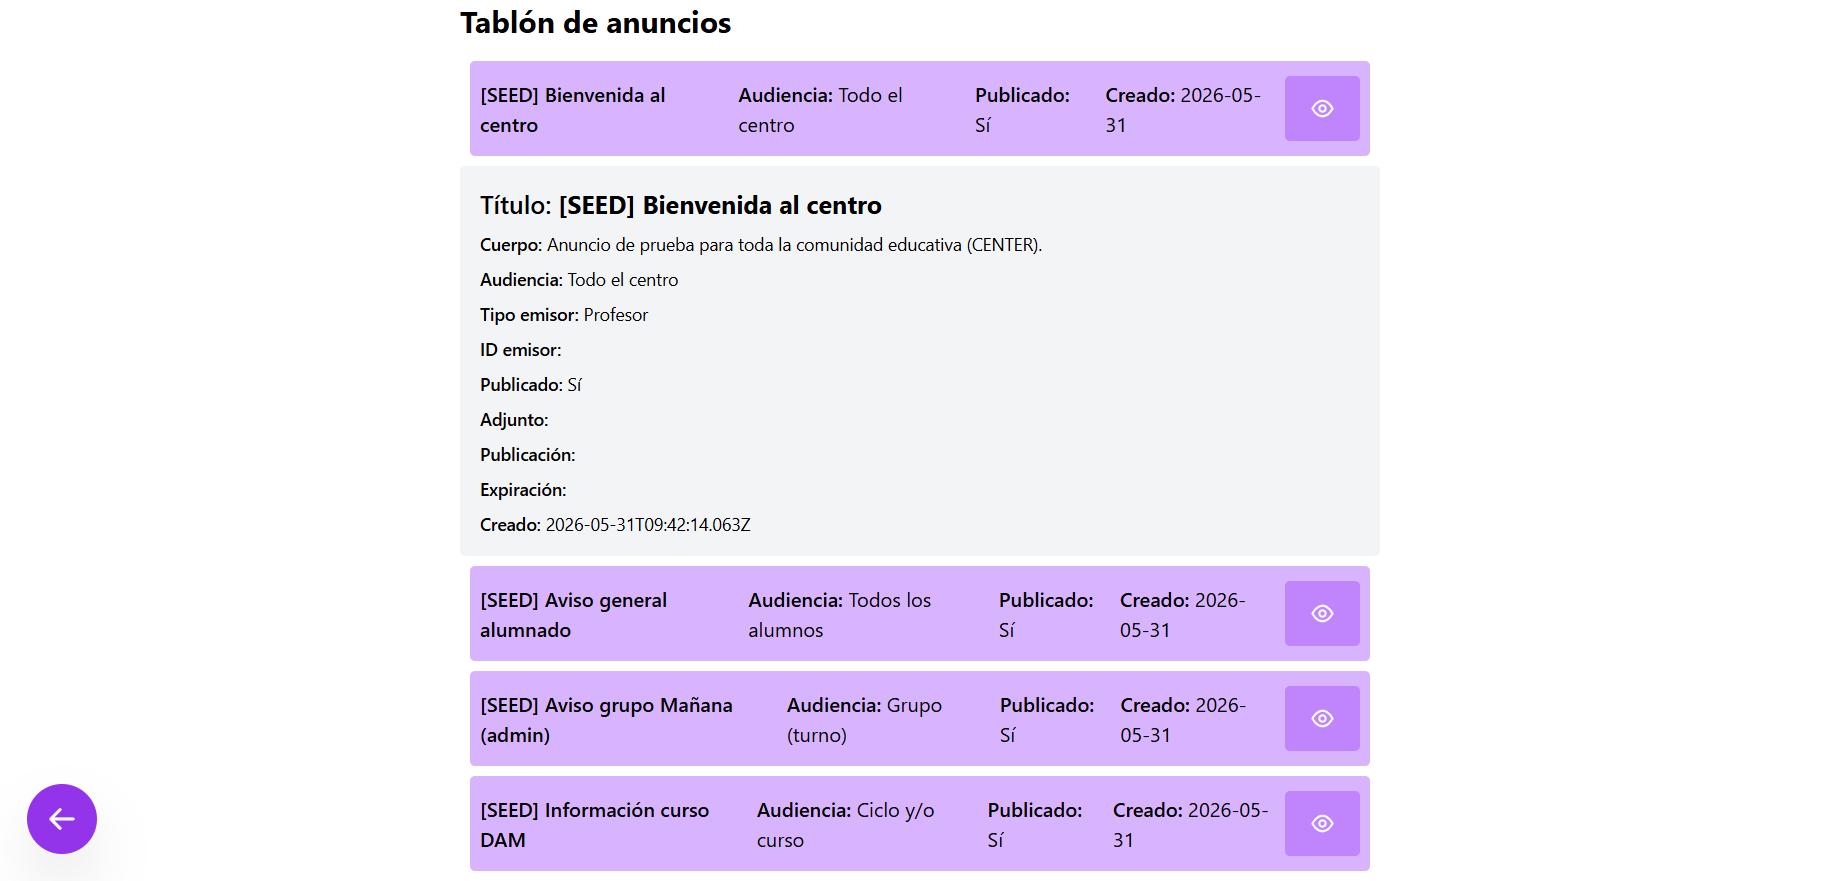
\includegraphics[keepaspectratio,alt={CAPTURA 19 --- Tablón de anuncios}]{../../assets/screenshots/manual-alumno/captura19-tablon.png}}
\caption{CAPTURA 19 --- Tablón de anuncios}
\end{figure}

\begin{center}\rule{0.5\linewidth}{0.5pt}\end{center}

\section{14. Mis evaluaciones (notas)}\label{mis-evaluaciones-notas}

Ruta: \textbf{Gestión → Evaluaciones} (\texttt{/mis-evaluaciones}).

\subsection{14.1 Tabla de calificaciones}\label{tabla-de-calificaciones}

\begin{itemize}
\tightlist
\item
  Tabla con \textbf{filas = asignaturas} y \textbf{columnas = periodos}
  de evaluación:

  \begin{itemize}
  \tightlist
  \item
    Evaluación inicial\\
  \item
    1º, 2º y 3º trimestre\\
  \item
    Nota final\\
  \end{itemize}
\item
  Las notas \textbf{inferiores a 5} suelen mostrarse en rojo; las
  aprobadas en verde.
\item
  La última fila muestra la \textbf{nota media} por periodo.
\end{itemize}

\begin{figure}
\centering
\pandocbounded{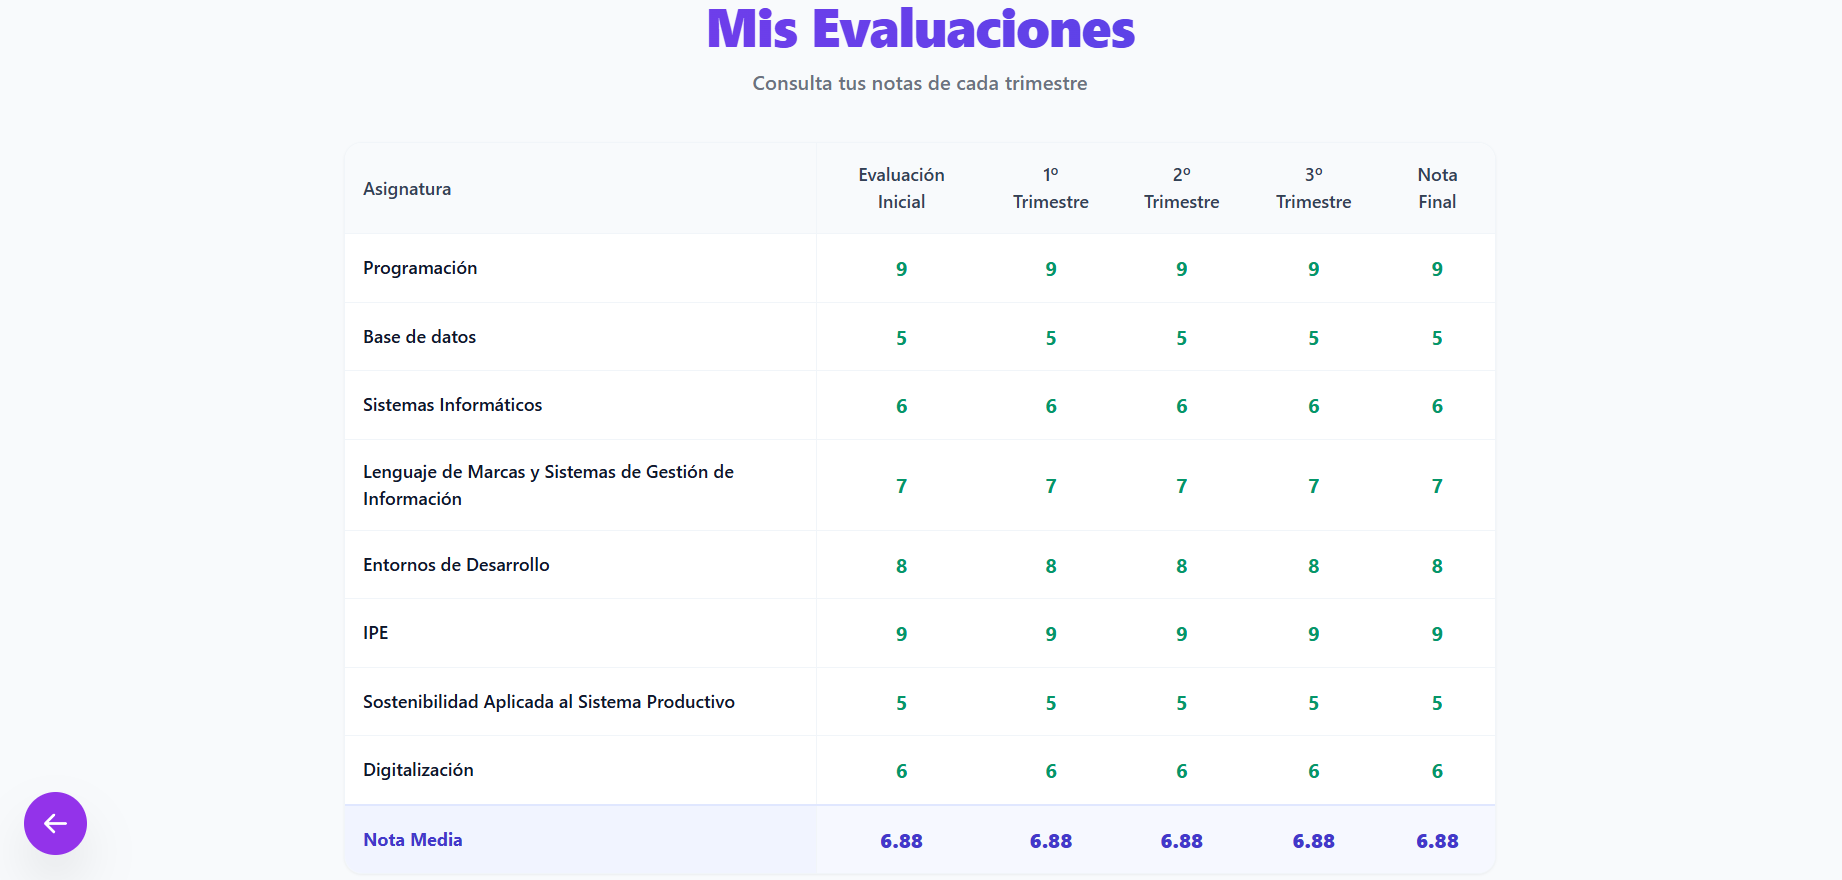
\includegraphics[keepaspectratio,alt={CAPTURA 20 --- Tabla de Mis evaluaciones}]{../../assets/screenshots/manual-alumno/captura20-evaluaciones.png}}
\caption{CAPTURA 20 --- Tabla de Mis evaluaciones}
\end{figure}

\subsection{14.2 Sin calificaciones}\label{sin-calificaciones}

Si el tutor o profesores aún no han introducido notas, verás: \emph{«Aún
no tienes calificaciones registradas»}.

\begin{center}\rule{0.5\linewidth}{0.5pt}\end{center}

\section{15. Flujo de trabajo recomendado
(resumen)}\label{flujo-de-trabajo-recomendado-resumen}

\begin{Shaded}
\begin{Highlighting}[]
\NormalTok{Login → Mi Espacio → Clases → Temario → Tarea → Entregar}
\NormalTok{                  ↘ Gestión → Ficha / Horario / Calendario / Tablón / Evaluaciones}
\end{Highlighting}
\end{Shaded}

\begin{center}\rule{0.5\linewidth}{0.5pt}\end{center}

\section{16. Preguntas frecuentes (FAQ)}\label{preguntas-frecuentes-faq}

\textbf{¿Puedo usar la app en el móvil?}\\
Sí; la interfaz es responsive, aunque algunas tablas se desplazan
horizontalmente.

\textbf{No veo ninguna asignatura}\\
Tu matrícula puede no estar activa; contacta con secretaría o
administración.

\textbf{He entregado pero sigue en PENDIENTE}\\
Comprueba que recibiste el mensaje de éxito; refresca la página. Si
persiste, avisa al profesor.

\textbf{Mi justificante fue rechazado}\\
Sube un nuevo documento válido o consulta con el profesor el motivo.

\textbf{¿Cómo cambio el idioma?}\\
Selector en la esquina superior izquierda de la cabecera.

\begin{center}\rule{0.5\linewidth}{0.5pt}\end{center}

\section{17. Glosario}\label{glosario}

{\def\LTcaptype{none} % do not increment counter
\begin{longtable}[]{@{}ll@{}}
\toprule\noalign{}
Término & Definición \\
\midrule\noalign{}
\endhead
\bottomrule\noalign{}
\endlastfoot
Temario & Conjunto de bloques y tareas de una asignatura \\
Entrega & Archivo o enlace que envías para una tarea \\
Trimestre & Periodo de evaluación académica \\
Justificante & Documento que acredita una ausencia \\
Tablón & Murales de avisos del centro \\
\end{longtable}
}

\begin{center}\rule{0.5\linewidth}{0.5pt}\end{center}

\emph{Fin del manual de alumno. Para incidencias técnicas, contacta con
el administrador del centro.}

\newpage

\chapter{Parte IV --- Manual de usuario:
Profesor}\label{parte-iv-manual-de-usuario-profesor}

\textbf{Versión:} 1.0 · \textbf{Aplicación:} Ziryab --- Plataforma
Educativa\\
\textbf{Rol:} Profesor (TEACHER)\\
\textbf{Última actualización:} junio 2026 · \textbf{Capturas:} incluidas
(26 y 27 pendientes)

\begin{center}\rule{0.5\linewidth}{0.5pt}\end{center}

\section{1. Introducción}\label{introducciuxf3n-1}

\textbf{Ziryab} permite al profesorado gestionar sus asignaturas: crear
tareas, revisar entregas, calificar, pasar lista, validar justificantes
de ausencia y, si actúas como \textbf{tutor/a de grupo}, registrar las
evaluaciones trimestrales de tus alumnos.

Este manual cubre \textbf{todas las funcionalidades del rol TEACHER}.

\begin{center}\rule{0.5\linewidth}{0.5pt}\end{center}

\section{2. Requisitos previos}\label{requisitos-previos-1}

{\def\LTcaptype{none} % do not increment counter
\begin{longtable}[]{@{}
  >{\raggedright\arraybackslash}p{(\linewidth - 2\tabcolsep) * \real{0.5500}}
  >{\raggedright\arraybackslash}p{(\linewidth - 2\tabcolsep) * \real{0.4500}}@{}}
\toprule\noalign{}
\begin{minipage}[b]{\linewidth}\raggedright
Requisito
\end{minipage} & \begin{minipage}[b]{\linewidth}\raggedright
Detalle
\end{minipage} \\
\midrule\noalign{}
\endhead
\bottomrule\noalign{}
\endlastfoot
Navegador & Chrome, Firefox, Edge o Safari actualizado \\
Credenciales & Cuenta de profesor con asignaturas asignadas en el
sistema \\
Rol tutor (opcional) & Necesario para la pantalla \textbf{Evaluaciones}
de grupo tutorizado \\
Idiomas & ES / EN / DE desde la cabecera \\
\end{longtable}
}

\begin{center}\rule{0.5\linewidth}{0.5pt}\end{center}

\section{3. Inicio de sesión}\label{inicio-de-sesiuxf3n-1}

El acceso es idéntico al del alumno:

\begin{enumerate}
\def\labelenumi{\arabic{enumi}.}
\tightlist
\item
  Abre la URL de Ziryab.
\item
  Introduce \textbf{email} y \textbf{contraseña}.
\item
  Pulsa el botón de acceso.
\end{enumerate}

\begin{figure}
\centering
\pandocbounded{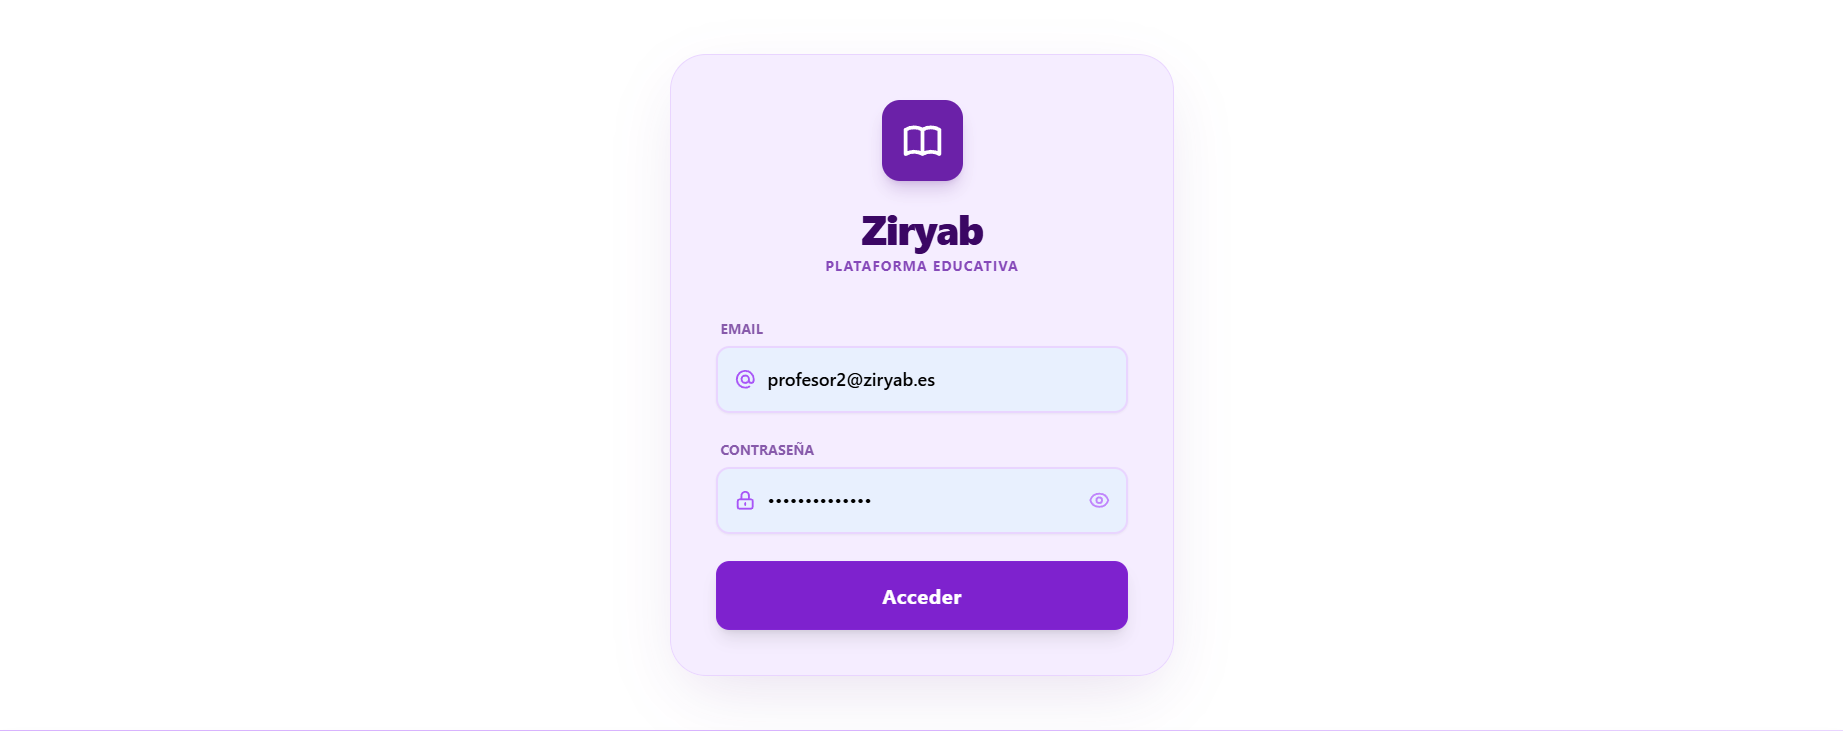
\includegraphics[keepaspectratio,alt={CAPTURA 1 --- Pantalla de login}]{../../assets/screenshots/manual-profesor/captura1-login.png}}
\caption{CAPTURA 1 --- Pantalla de login}
\end{figure}

Tras un login correcto con rol \textbf{TEACHER}, entrarás al
\textbf{Dashboard (Mi Espacio)} con las mismas dos tarjetas principales,
pero la tarjeta \textbf{Clases} te llevará a \textbf{Mis clases} del
profesor.

\begin{center}\rule{0.5\linewidth}{0.5pt}\end{center}

\section{4. Interfaz general
(cabecera)}\label{interfaz-general-cabecera-1}

La cabecera morada incluye:

{\def\LTcaptype{none} % do not increment counter
\begin{longtable}[]{@{}ll@{}}
\toprule\noalign{}
Elemento & Función \\
\midrule\noalign{}
\endhead
\bottomrule\noalign{}
\endlastfoot
Selector de idioma & Cambia el idioma de la interfaz \\
\textbf{Ziryab} (centro) & Vuelve al Dashboard \\
Notificaciones & Avisos de entregas, justificantes, etc. \\
Perfil (nombre + «PROFESOR») & Menú con \textbf{Cerrar sesión} \\
\end{longtable}
}

\begin{figure}
\centering
\pandocbounded{
\includegraphics[keepaspectratio,alt={CAPTURA 2 --- Cabecera con rol Profesor visible}]{../../assets/screenshots/manual-profesor/captura2-cabecera.png}}
\caption{CAPTURA 2 --- Cabecera con rol Profesor visible}
\end{figure}

\subsection{4.1 Notificaciones y cierre de
sesión}\label{notificaciones-y-cierre-de-sesiuxf3n}

\begin{itemize}
\tightlist
\item
  \textbf{Campana:} abre el listado de notificaciones; puedes marcarlas
  como leídas.
\item
  \textbf{Perfil → Cerrar sesión:} finaliza la sesión de forma segura.
\end{itemize}

\begin{figure}
\centering
\pandocbounded{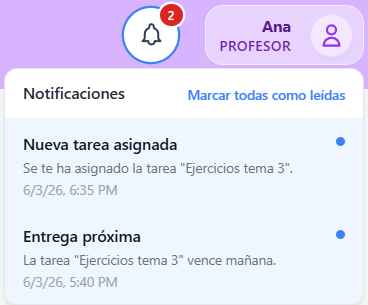
\includegraphics[keepaspectratio,alt={CAPTURA 3 --- Panel de notificaciones}]{../../assets/screenshots/manual-profesor/captura3-notificaciones.png}}
\caption{CAPTURA 3 --- Panel de notificaciones}
\end{figure}

\begin{figure}
\centering
\pandocbounded{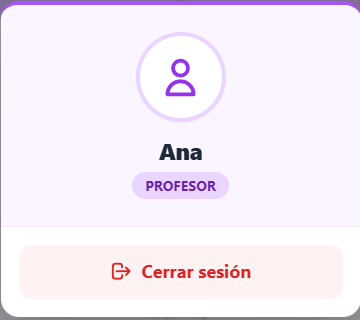
\includegraphics[keepaspectratio,alt={CAPTURA 4 --- Modal de perfil}]{../../assets/screenshots/manual-profesor/captura4-modal.png}}
\caption{CAPTURA 4 --- Modal de perfil}
\end{figure}

\begin{center}\rule{0.5\linewidth}{0.5pt}\end{center}

\section{5. Panel principal --- «Mi
Espacio»}\label{panel-principal-mi-espacio}

Pantalla inicial con dos accesos:

{\def\LTcaptype{none} % do not increment counter
\begin{longtable}[]{@{}
  >{\raggedright\arraybackslash}p{(\linewidth - 2\tabcolsep) * \real{0.3214}}
  >{\raggedright\arraybackslash}p{(\linewidth - 2\tabcolsep) * \real{0.6786}}@{}}
\toprule\noalign{}
\begin{minipage}[b]{\linewidth}\raggedright
Tarjeta
\end{minipage} & \begin{minipage}[b]{\linewidth}\raggedright
Destino (profesor)
\end{minipage} \\
\midrule\noalign{}
\endhead
\bottomrule\noalign{}
\endlastfoot
\textbf{Clases} & \texttt{/clases-profesor} --- Asignaturas que
impartes \\
\textbf{Gestión} & \texttt{/gestion} --- Ficha, horario, calendario,
tablón, evaluaciones \\
\end{longtable}
}

\begin{figure}
\centering
\pandocbounded{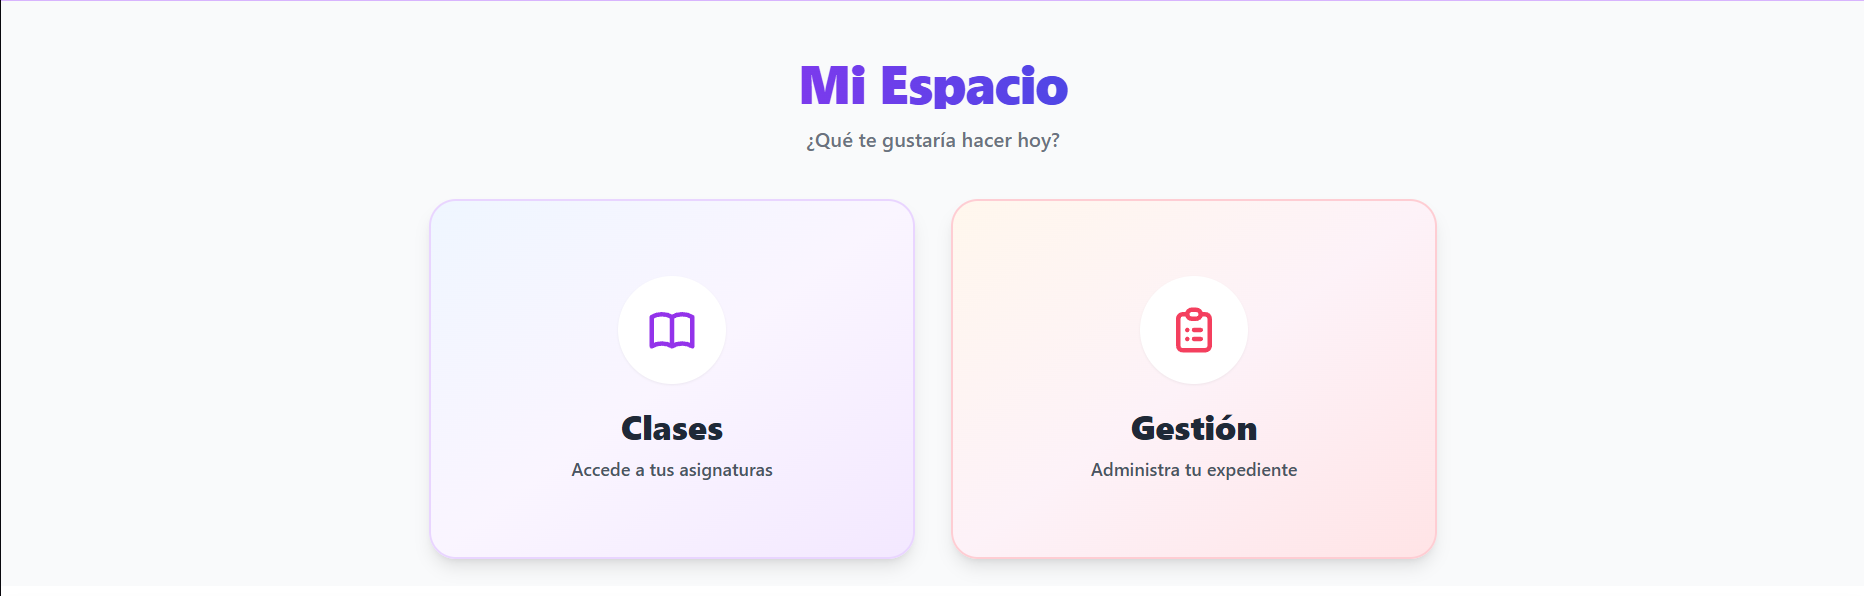
\includegraphics[keepaspectratio,alt={CAPTURA 5 --- Dashboard del profesor}]{../../assets/screenshots/manual-profesor/captura5-dashboard.png}}
\caption{CAPTURA 5 --- Dashboard del profesor}
\end{figure}

\begin{center}\rule{0.5\linewidth}{0.5pt}\end{center}

\section{6. Mis clases (asignaturas
asignadas)}\label{mis-clases-asignaturas-asignadas}

Ruta: \textbf{Mi Espacio → Clases} (\texttt{/clases-profesor}).

\subsection{6.1 Listado}\label{listado}

Cada tarjeta representa una \textbf{asignación} (asignatura + grupo +
ciclo) y muestra:

\begin{itemize}
\tightlist
\item
  Nombre de la \textbf{asignatura}
\item
  \textbf{Ciclo} y \textbf{grupo}
\item
  Dos acciones:

  \begin{enumerate}
  \def\labelenumi{\arabic{enumi}.}
  \tightlist
  \item
    \textbf{Gestionar temario} --- Material, tareas y asistencia de esa
    asignatura
  \item
    \textbf{Menú de clase} --- Acceso rápido a tareas y justificaciones
  \end{enumerate}
\end{itemize}

\begin{figure}
\centering
\pandocbounded{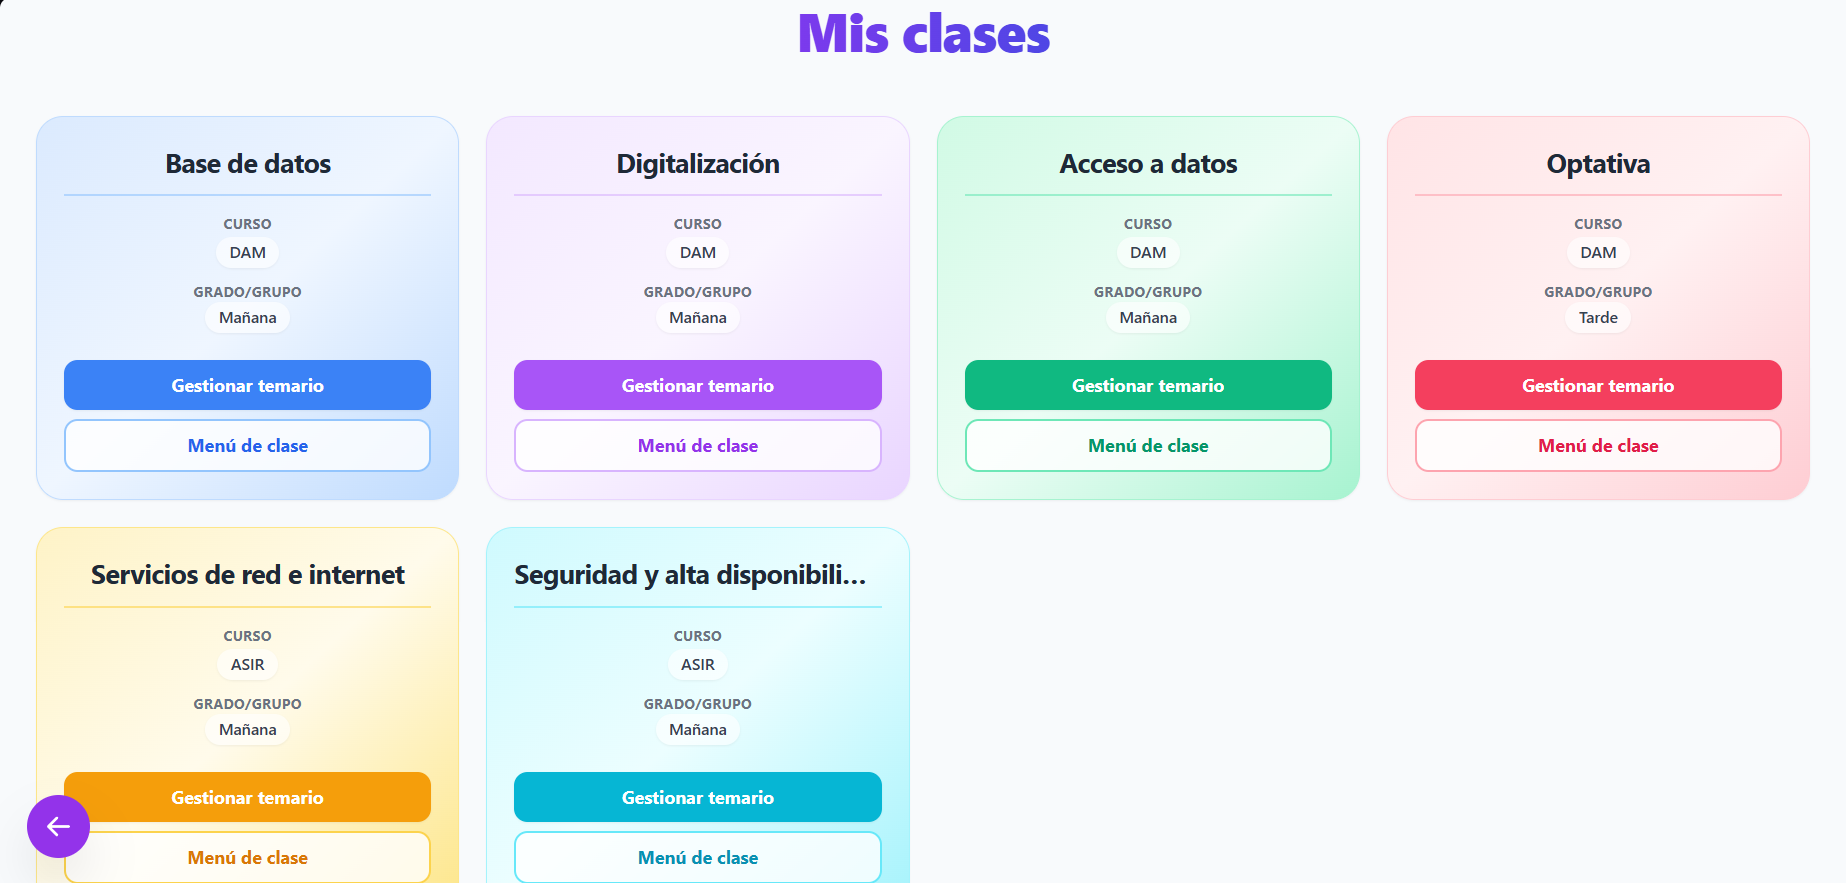
\includegraphics[keepaspectratio,alt={CAPTURA 6 --- Listado «Mis clases» con dos botones por tarjeta}]{../../assets/screenshots/manual-profesor/captura6-clases.png}}
\caption{CAPTURA 6 --- Listado «Mis clases» con dos botones por tarjeta}
\end{figure}

\subsection{6.2 Sin asignaturas}\label{sin-asignaturas}

Si no tienes asignaturas asignadas, verás un mensaje informativo.
Contacta con administración para revisar tu carga docente en el sistema.

\begin{center}\rule{0.5\linewidth}{0.5pt}\end{center}

\section{7. Programación / Temario del
profesor}\label{programaciuxf3n-temario-del-profesor}

Ruta: \textbf{Gestionar temario} → \texttt{/temario-profesor/:claseId}

\subsection{7.1 Vista general}\label{vista-general}

\begin{itemize}
\tightlist
\item
  Título \textbf{Programación}.
\item
  Botón \textbf{Pasar lista} (esquina superior derecha): abre el modal
  de asistencia.
\item
  Bloques por tipo de contenido (teoría, exámenes, proyectos, prácticas,
  deberes), igual que ve el alumno pero con \textbf{controles de
  profesor}.
\end{itemize}

\begin{figure}
\centering
\pandocbounded{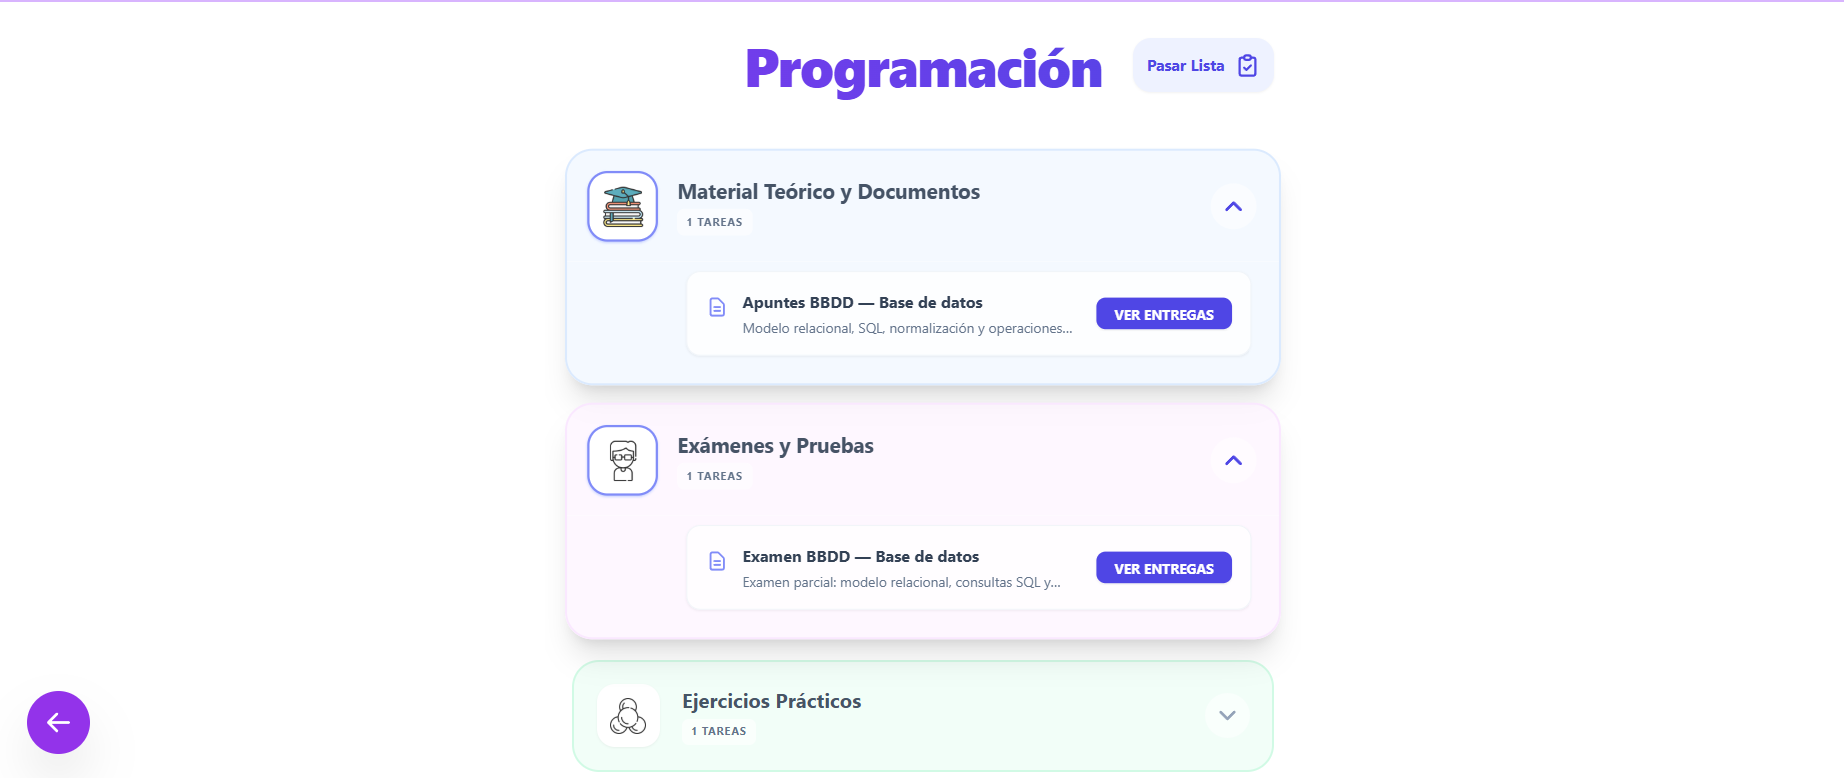
\includegraphics[keepaspectratio,alt={CAPTURA 7 --- Temario del profesor con botón Pasar lista}]{../../assets/screenshots/manual-profesor/captura8-temario.png}}
\caption{CAPTURA 7 --- Temario del profesor con botón Pasar lista}
\end{figure}

\subsection{7.2 Gestionar tareas dentro del
temario}\label{gestionar-tareas-dentro-del-temario}

En cada bloque expandido, cada tarea muestra:

\begin{itemize}
\tightlist
\item
  Título y descripción
\item
  \textbf{Ver archivo base} --- Abre el adjunto que subiste al crear la
  tarea
\item
  \textbf{Ver entregas} --- Ir al listado de entregas de los alumnos
\end{itemize}

\subsection{7.3 Pasar lista (asistencia)}\label{pasar-lista-asistencia}

\begin{enumerate}
\def\labelenumi{\arabic{enumi}.}
\tightlist
\item
  Pulsa \textbf{Pasar lista}.
\item
  Se abre un \textbf{modal} con la lista de alumnos matriculados.
\item
  Para cada alumno, selecciona el estado:

  \begin{itemize}
  \tightlist
  \item
    \textbf{Presente}
  \item
    \textbf{Ausente}
  \item
    \textbf{Retraso}
  \item
    \textbf{Justificado}
  \end{itemize}
\item
  Pulsa \textbf{Guardar asistencia}.
\item
  Mensaje de confirmación si se guardó correctamente.
\end{enumerate}

\begin{figure}
\centering
\pandocbounded{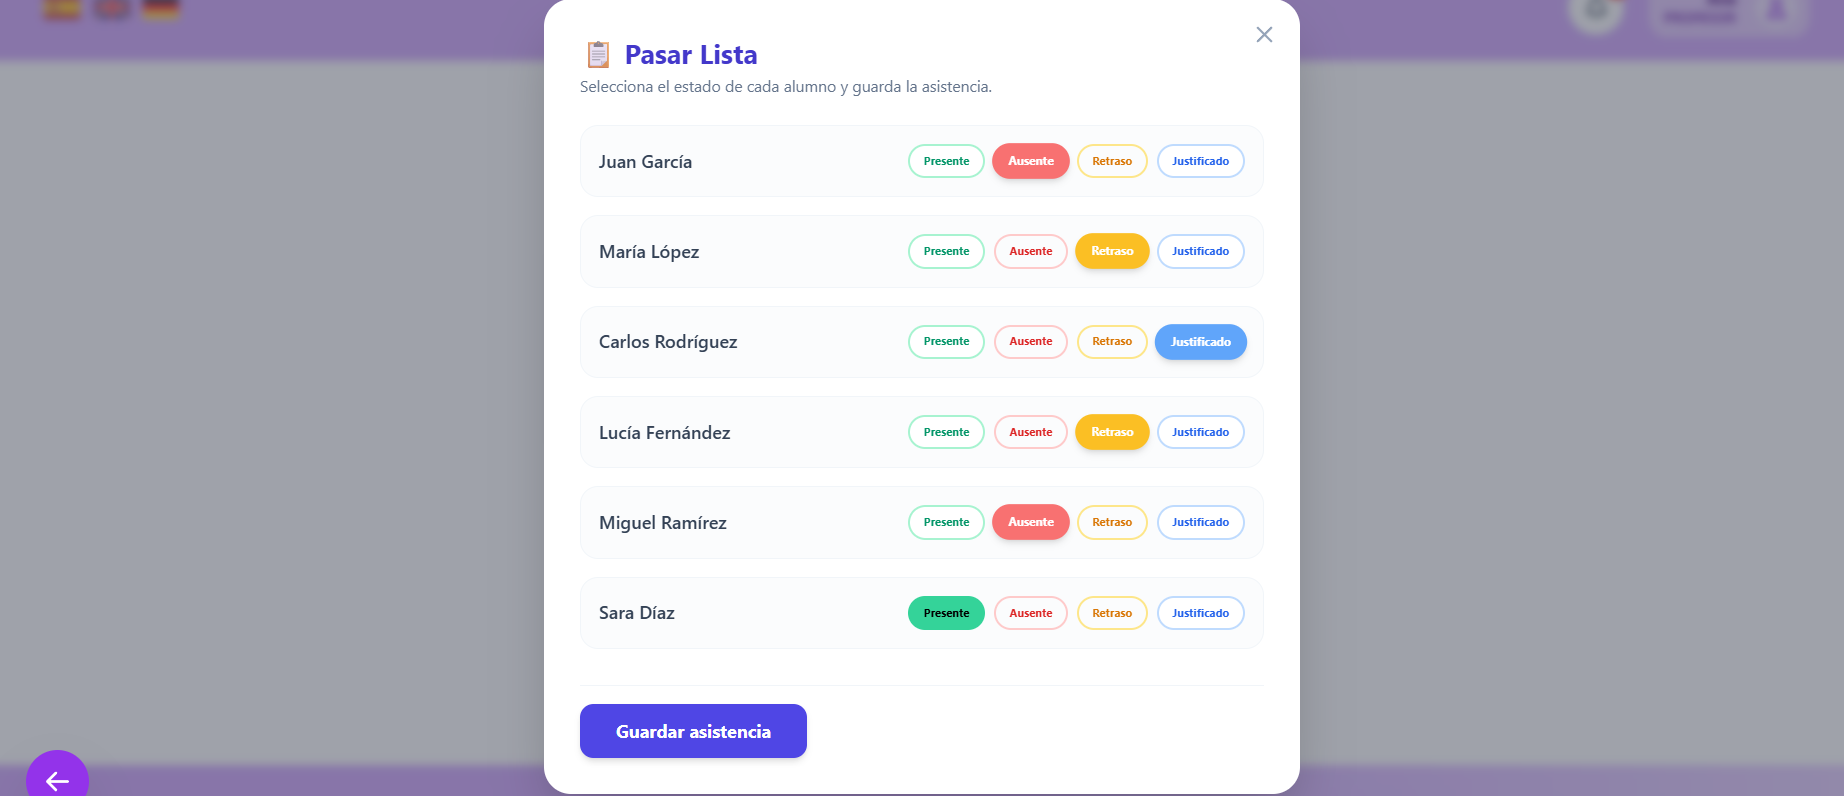
\includegraphics[keepaspectratio,alt={CAPTURA 9 --- Modal de asistencia con lista de alumnos y estados}]{../../assets/screenshots/manual-profesor/captura7-pasar_lista.png}}
\caption{CAPTURA 9 --- Modal de asistencia con lista de alumnos y
estados}
\end{figure}

\begin{figure}
\centering
\pandocbounded{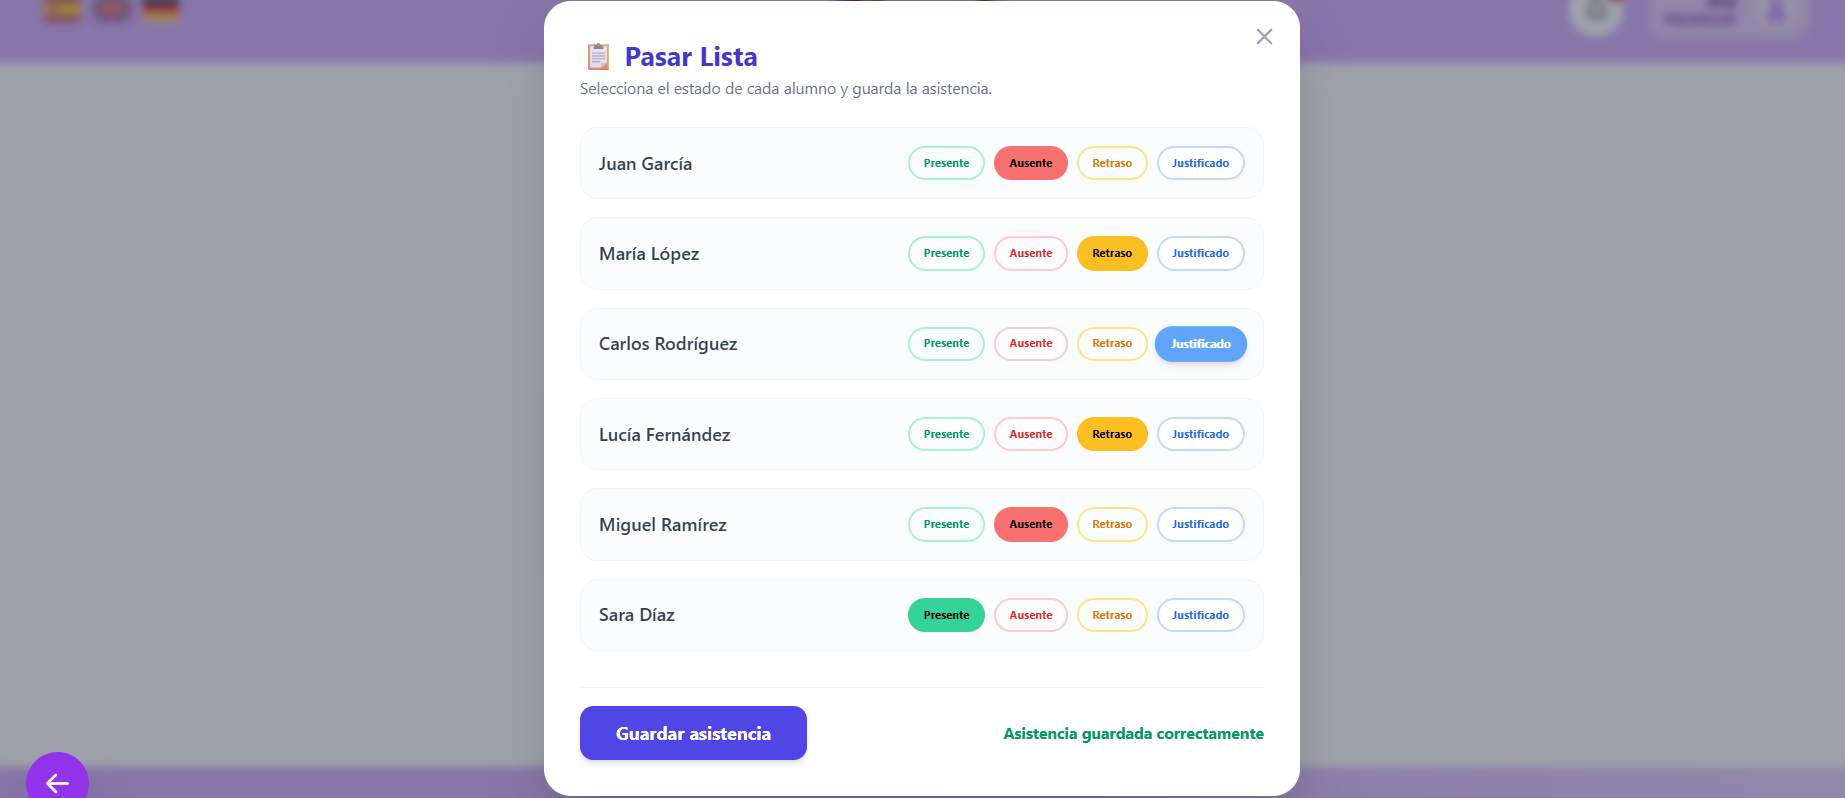
\includegraphics[keepaspectratio,alt={CAPTURA 10 --- Asistencia guardada correctamente}]{../../assets/screenshots/manual-profesor/captura10-lista_mandada.png}}
\caption{CAPTURA 10 --- Asistencia guardada correctamente}
\end{figure}

\textbf{Nota:} Debes pasar lista en la sesión correspondiente al día; si
no hay alumnos matriculados, el sistema lo indicará.

\begin{center}\rule{0.5\linewidth}{0.5pt}\end{center}

\section{8. Menú de clase}\label{menuxfa-de-clase}

Ruta: \textbf{Menú de clase} desde una tarjeta →
\texttt{/menu-clase/:idTeacherAssignment}

Pantalla intermedia con \textbf{dos opciones}:

{\def\LTcaptype{none} % do not increment counter
\begin{longtable}[]{@{}
  >{\raggedright\arraybackslash}p{(\linewidth - 4\tabcolsep) * \real{0.2963}}
  >{\raggedright\arraybackslash}p{(\linewidth - 4\tabcolsep) * \real{0.4815}}
  >{\raggedright\arraybackslash}p{(\linewidth - 4\tabcolsep) * \real{0.2222}}@{}}
\toprule\noalign{}
\begin{minipage}[b]{\linewidth}\raggedright
Opción
\end{minipage} & \begin{minipage}[b]{\linewidth}\raggedright
Descripción
\end{minipage} & \begin{minipage}[b]{\linewidth}\raggedright
Ruta
\end{minipage} \\
\midrule\noalign{}
\endhead
\bottomrule\noalign{}
\endlastfoot
\textbf{Tareas} & Crear y listar tareas de la asignación &
\texttt{/tareas/:idTeacherAssignment} \\
\textbf{Justificaciones} & Revisar justificantes de faltas &
\texttt{/ficha-profesor} (vista de justificaciones) \\
\end{longtable}
}

\begin{figure}
\centering
\pandocbounded{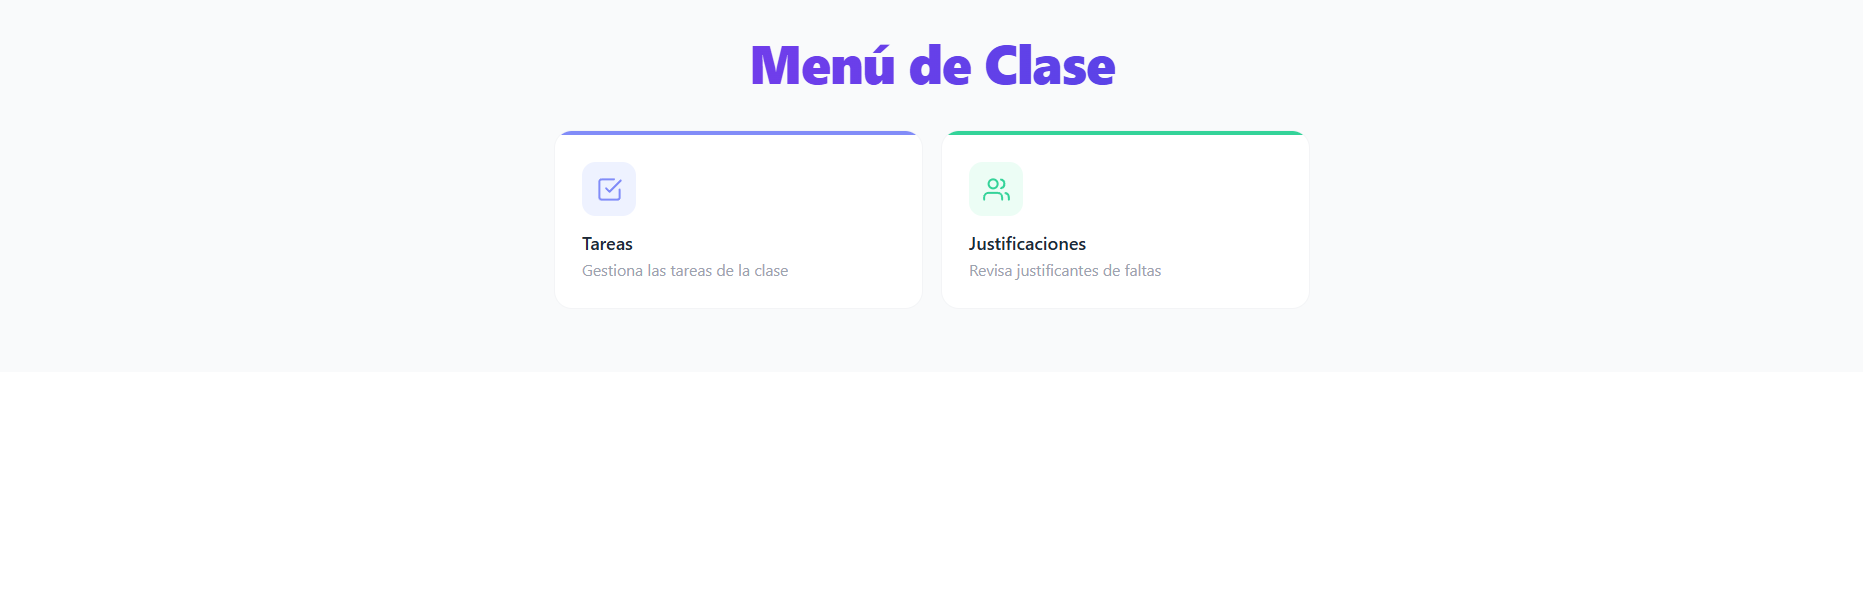
\includegraphics[keepaspectratio,alt={CAPTURA 11 --- Menú de clase con tarjetas Tareas y Justificaciones}]{../../assets/screenshots/manual-profesor/captura11-menu_clase.png}}
\caption{CAPTURA 11 --- Menú de clase con tarjetas Tareas y
Justificaciones}
\end{figure}

\begin{center}\rule{0.5\linewidth}{0.5pt}\end{center}

\section{9. Gestión de tareas}\label{gestiuxf3n-de-tareas}

Ruta: \textbf{Menú de clase → Tareas}
(\texttt{/tareas/:idTeacherAssignment}).

\subsection{9.1 Listado agrupado}\label{listado-agrupado}

\begin{itemize}
\tightlist
\item
  Las tareas se agrupan por \textbf{tipo} (deberes, práctica, teoría,
  proyecto, examen) con código de color.
\item
  En la cabecera: número total de tareas y botón \textbf{+ Crear tarea}.
\item
  Cada ítem permite ver detalle y acciones según el componente de lista.
\end{itemize}

\begin{figure}
\centering
\pandocbounded{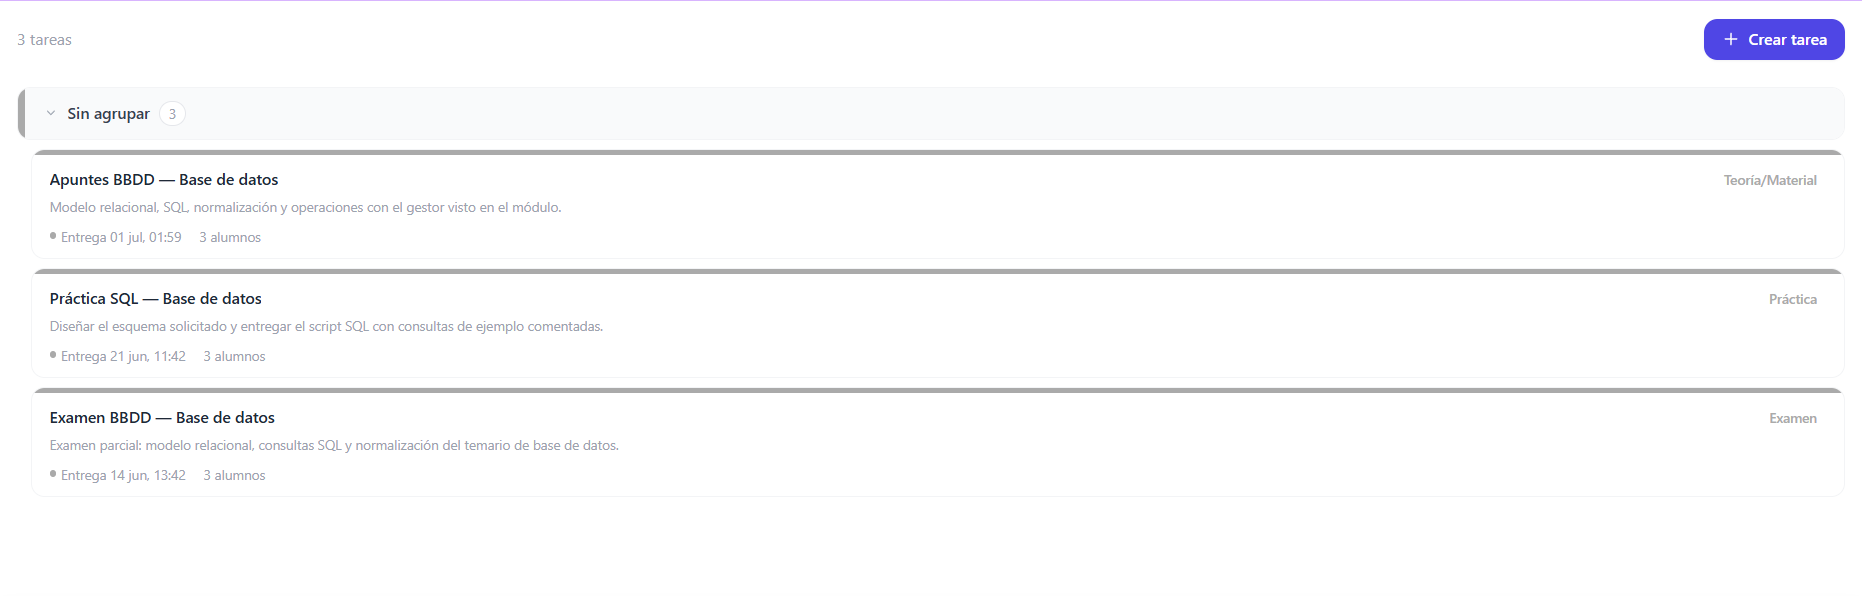
\includegraphics[keepaspectratio,alt={CAPTURA 12 --- Lista de tareas agrupadas con botón Crear tarea}]{../../assets/screenshots/manual-profesor/captura12-tareas_agrupadas.png}}
\caption{CAPTURA 12 --- Lista de tareas agrupadas con botón Crear tarea}
\end{figure}

\subsection{9.2 Crear una nueva tarea}\label{crear-una-nueva-tarea}

\begin{enumerate}
\def\labelenumi{\arabic{enumi}.}
\tightlist
\item
  Pulsa \textbf{Crear tarea} (botón indigo con icono +).
\item
  Se abre el formulario modal \textbf{Crear nueva tarea}.
\end{enumerate}

Campos del formulario:

{\def\LTcaptype{none} % do not increment counter
\begin{longtable}[]{@{}
  >{\raggedright\arraybackslash}p{(\linewidth - 4\tabcolsep) * \real{0.2121}}
  >{\raggedright\arraybackslash}p{(\linewidth - 4\tabcolsep) * \real{0.3939}}
  >{\raggedright\arraybackslash}p{(\linewidth - 4\tabcolsep) * \real{0.3939}}@{}}
\toprule\noalign{}
\begin{minipage}[b]{\linewidth}\raggedright
Campo
\end{minipage} & \begin{minipage}[b]{\linewidth}\raggedright
Obligatorio
\end{minipage} & \begin{minipage}[b]{\linewidth}\raggedright
Descripción
\end{minipage} \\
\midrule\noalign{}
\endhead
\bottomrule\noalign{}
\endlastfoot
Título & Sí & Nombre visible para el alumno \\
Descripción & No & Instrucciones de la actividad \\
Tipo & Sí & Deberes, práctica, teoría/material, proyecto, examen \\
Fecha de inicio & Sí & Cuándo se publica \\
Fecha límite & Sí & Deadline de entrega \\
Fichero adjunto & No & Material de apoyo (PDF, DOCX, ZIP, PNG, JPG; máx.
10 MB) \\
Permite entrega tardía & Según diseño & Si está activo, los alumnos
pueden entregar fuera de plazo (marcado LATE) \\
\end{longtable}
}

\begin{enumerate}
\def\labelenumi{\arabic{enumi}.}
\setcounter{enumi}{2}
\tightlist
\item
  Opcional: arrastra un archivo o selecciónalo.
\item
  Pulsa \textbf{Crear tarea}.
\item
  Tras el éxito, la tarea aparecerá en el listado y en el
  \textbf{temario} del alumno.
\end{enumerate}

\begin{figure}
\centering
\pandocbounded{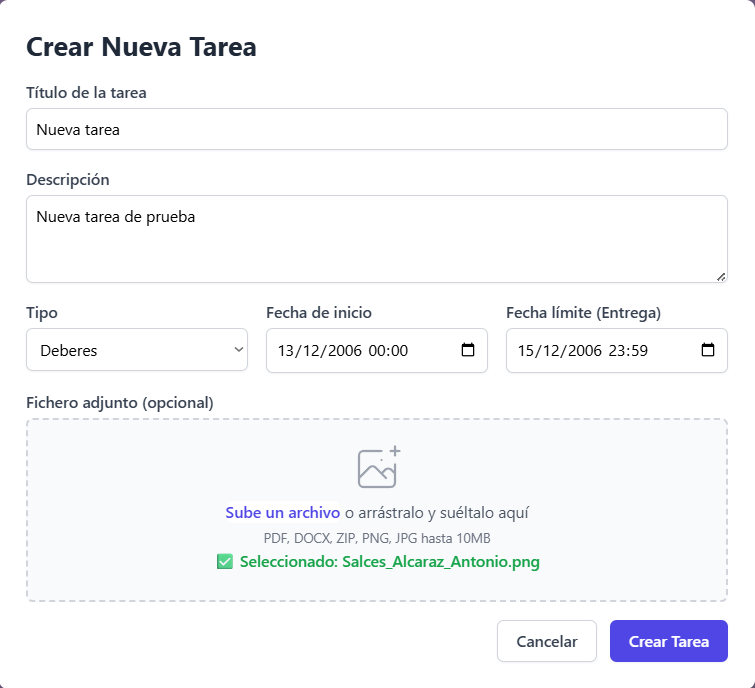
\includegraphics[keepaspectratio,alt={CAPTURA 13 --- Formulario Crear nueva tarea y confirmación}]{../../assets/screenshots/manual-profesor/captura13-guardar_tarea.png}}
\caption{CAPTURA 13 --- Formulario Crear nueva tarea y confirmación}
\end{figure}

\subsection{9.3 Errores al crear tarea}\label{errores-al-crear-tarea}

\begin{itemize}
\tightlist
\item
  Archivo mayor de 10 MB → error de tamaño.
\item
  Error de servidor → revisa conexión y reintenta.
\end{itemize}

\begin{center}\rule{0.5\linewidth}{0.5pt}\end{center}

\section{10. Entregas de los alumnos}\label{entregas-de-los-alumnos}

Ruta: \textbf{Temario → Ver entregas} o desde detalle de tarea →
\texttt{/tarea/:taskId/entregas}

\subsection{10.1 Pantalla de entregas}\label{pantalla-de-entregas}

Información mostrada:

\begin{itemize}
\tightlist
\item
  Título de la tarea y \textbf{fecha límite}
\item
  Tabla o listado con columnas: \textbf{Alumno}, \textbf{Estado},
  \textbf{Fecha entrega}, \textbf{Nota}, \textbf{Acciones}
\end{itemize}

Estados habituales:

{\def\LTcaptype{none} % do not increment counter
\begin{longtable}[]{@{}ll@{}}
\toprule\noalign{}
Estado & Significado \\
\midrule\noalign{}
\endhead
\bottomrule\noalign{}
\endlastfoot
Pendiente & Sin entrega \\
Entregada & Entrega a tiempo \\
Retraso / Entregada tarde & Fuera de plazo permitido \\
Calificada & Ya tiene nota \\
No entregado & Plazo cerrado sin entrega \\
\end{longtable}
}

\begin{figure}
\centering
\pandocbounded{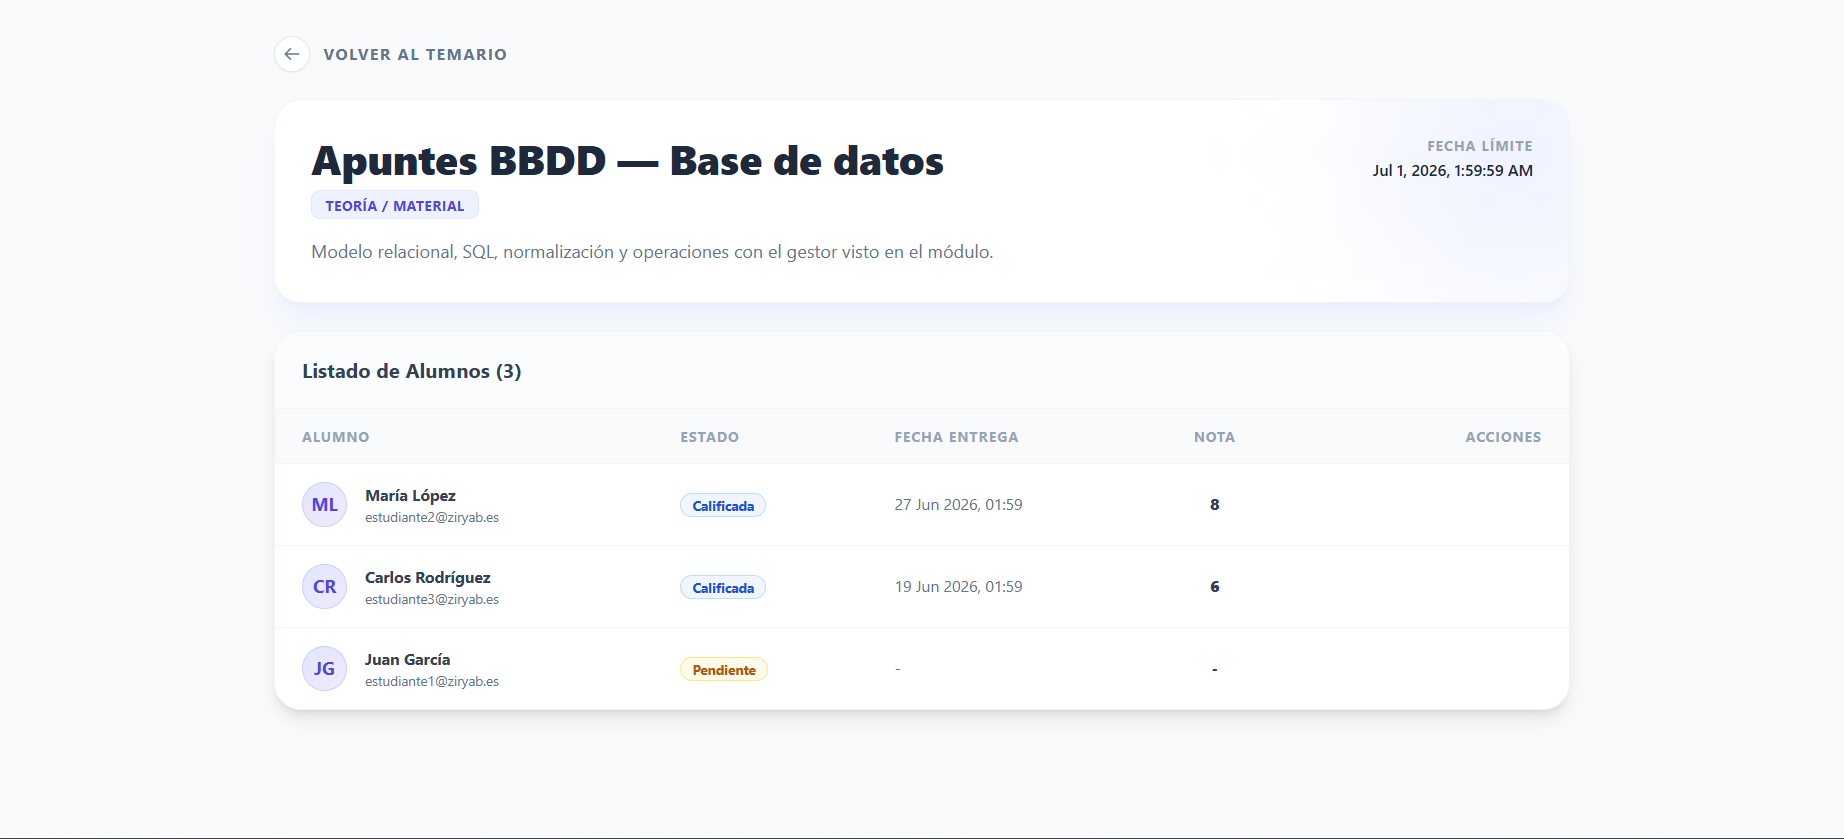
\includegraphics[keepaspectratio,alt={CAPTURA 15 --- Listado de entregas con varios estados}]{../../assets/screenshots/manual-profesor/captura15-listado_tareas.png}}
\caption{CAPTURA 15 --- Listado de entregas con varios estados}
\end{figure}

\subsection{10.2 Acciones por entrega}\label{acciones-por-entrega}

\begin{itemize}
\tightlist
\item
  \textbf{Abrir archivo/enlace} de la resolución del alumno (si
  entregó).
\item
  \textbf{Calificar} o \textbf{Editar nota} --- Abre la pantalla de
  corrección.
\end{itemize}

\begin{center}\rule{0.5\linewidth}{0.5pt}\end{center}

\section{11. Calificar una entrega}\label{calificar-una-entrega}

Ruta: \texttt{/calificar-tarea/:id} (ID de la entrega del alumno)

\subsection{11.1 Datos de la entrega}\label{datos-de-la-entrega}

La pantalla muestra:

\begin{itemize}
\tightlist
\item
  Nombre del \textbf{alumno}
\item
  \textbf{Tarea} evaluada
\item
  \textbf{Momento de entrega} (fecha/hora)
\item
  \textbf{Archivo entregado} --- enlace Ver / Descargar
\end{itemize}

\subsection{11.2 Formulario de
corrección}\label{formulario-de-correcciuxf3n}

{\def\LTcaptype{none} % do not increment counter
\begin{longtable}[]{@{}ll@{}}
\toprule\noalign{}
Campo & Reglas \\
\midrule\noalign{}
\endhead
\bottomrule\noalign{}
\endlastfoot
Calificación (0--10) & Obligatoria; valor entre 0 y 10 \\
Comentarios y feedback & Opcional; visible para el alumno \\
\end{longtable}
}

\begin{enumerate}
\def\labelenumi{\arabic{enumi}.}
\tightlist
\item
  Introduce la \textbf{nota}.
\item
  Opcional: escribe observaciones en \textbf{Feedback}.
\item
  Pulsa \textbf{Guardar calificación}.
\end{enumerate}

\begin{figure}
\centering
\pandocbounded{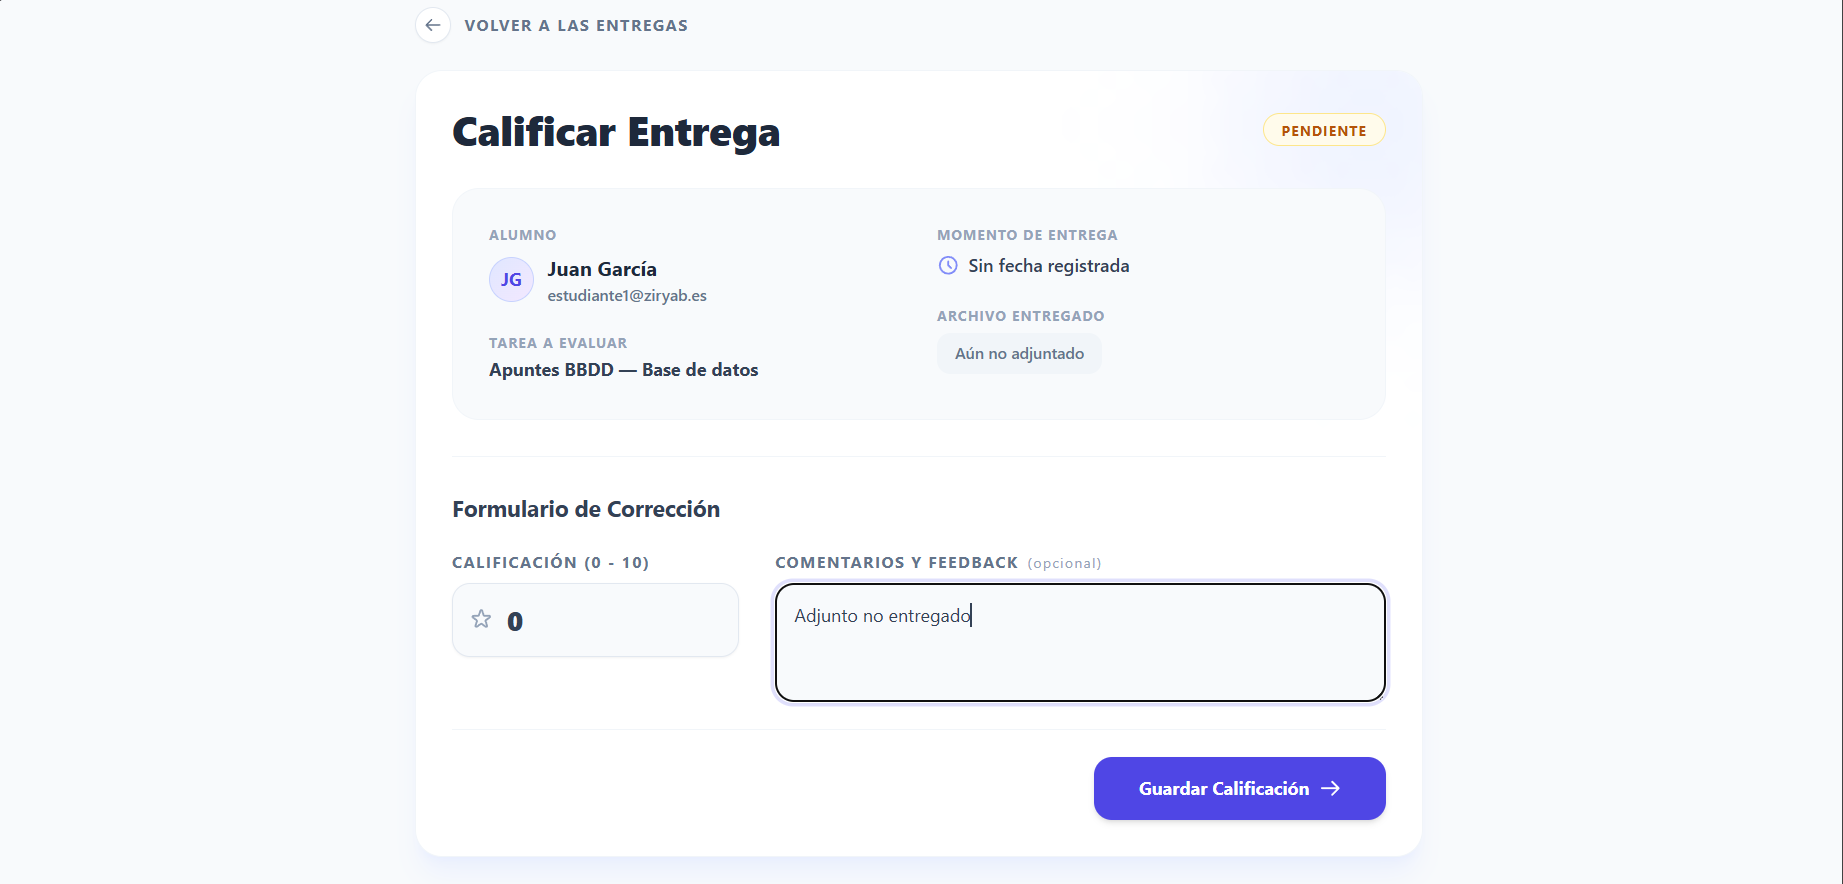
\includegraphics[keepaspectratio,alt={CAPTURA 16 --- Pantalla Calificar entrega}]{../../assets/screenshots/manual-profesor/captura16-calificar_entrega.png}}
\caption{CAPTURA 16 --- Pantalla Calificar entrega}
\end{figure}

El alumno verá la nota en su detalle de tarea y en el temario (estado
CALIFICADA).

\begin{center}\rule{0.5\linewidth}{0.5pt}\end{center}

\section{12. Justificaciones de faltas}\label{justificaciones-de-faltas}

Ruta: \textbf{Menú de clase → Justificaciones} o ficha de profesor
(\texttt{/ficha-profesor}).

\subsection{12.1 Justificaciones
pendientes}\label{justificaciones-pendientes}

\begin{itemize}
\tightlist
\item
  Listado de alumnos que han subido un \textbf{justificante} en estado
  pendiente.
\item
  Por cada fila: nombre del alumno, fecha/hora de la sesión, asignatura.
\item
  Acciones:

  \begin{itemize}
  \tightlist
  \item
    \textbf{Ver archivo} --- Abre el documento subido (PDF/imagen)
  \item
    \textbf{Aceptar} --- La falta pasa a justificada
  \item
    \textbf{Rechazar} --- El justificante se rechaza; el alumno puede
    volver a enviar otro
  \end{itemize}
\end{itemize}

\begin{figure}
\centering
\pandocbounded{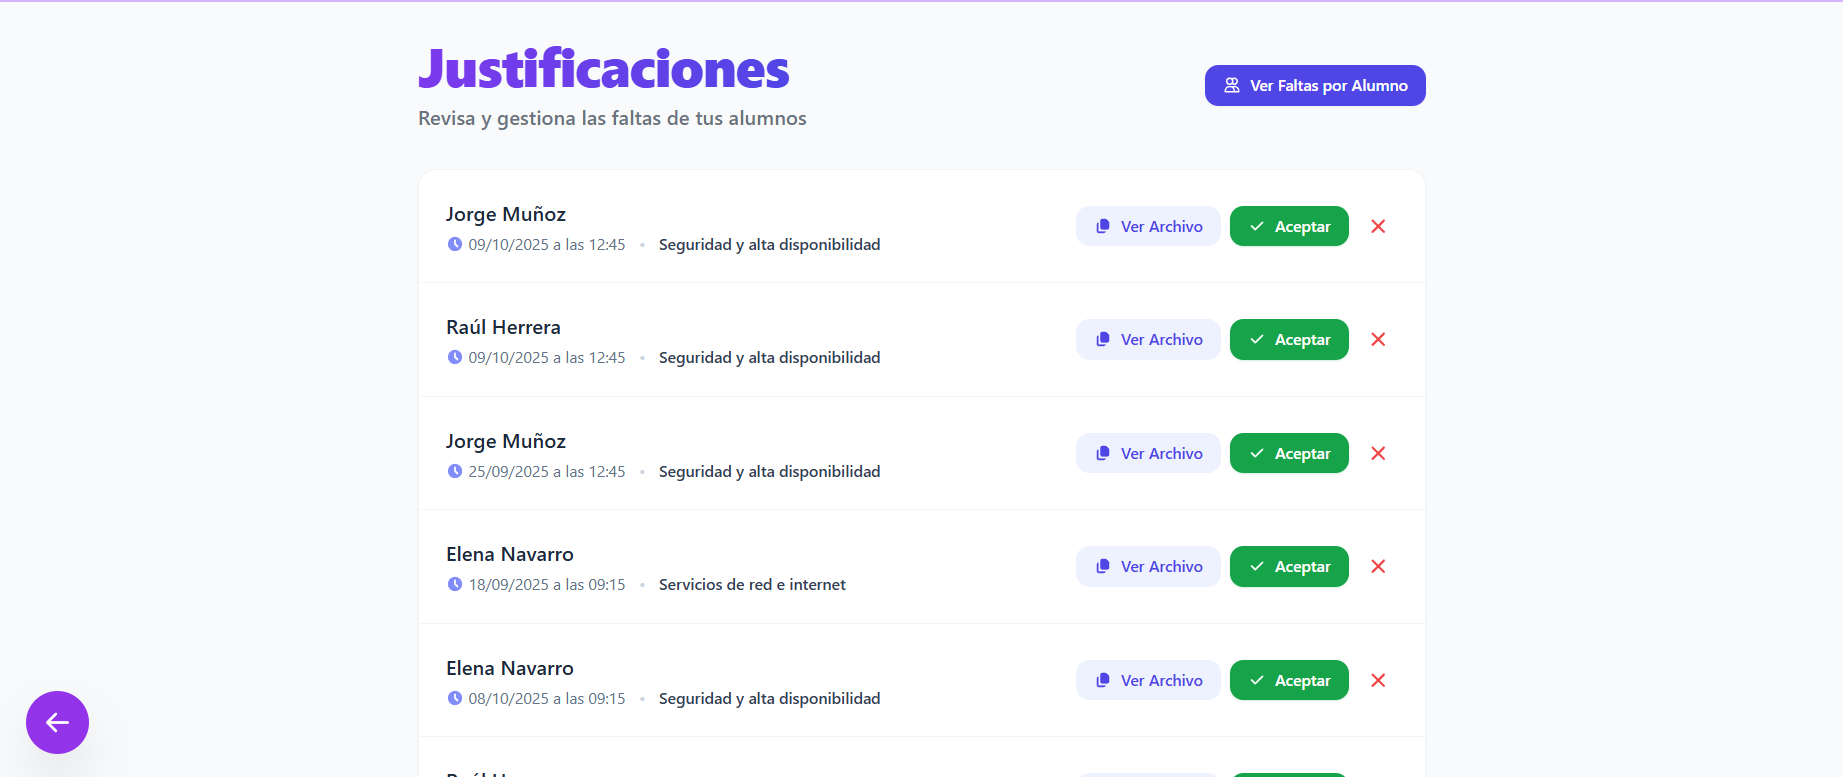
\includegraphics[keepaspectratio,alt={CAPTURA 19 --- Lista de justificaciones pendientes}]{../../assets/screenshots/manual-profesor/captura19-justificaciones_pendientes.png}}
\caption{CAPTURA 19 --- Lista de justificaciones pendientes}
\end{figure}

\subsection{12.2 Sin pendientes}\label{sin-pendientes}

Mensaje: \emph{«Todo al día»} / \emph{«No hay nuevas justificaciones
pendientes de revisar»}.

\subsection{12.3 Ver faltas por alumno}\label{ver-faltas-por-alumno}

\begin{itemize}
\tightlist
\item
  Botón \textbf{Ver faltas por alumno} (parte superior).
\item
  Abre un modal para consultar el historial de ausencias de un
  estudiante concreto.
\end{itemize}

\begin{figure}
\centering
\pandocbounded{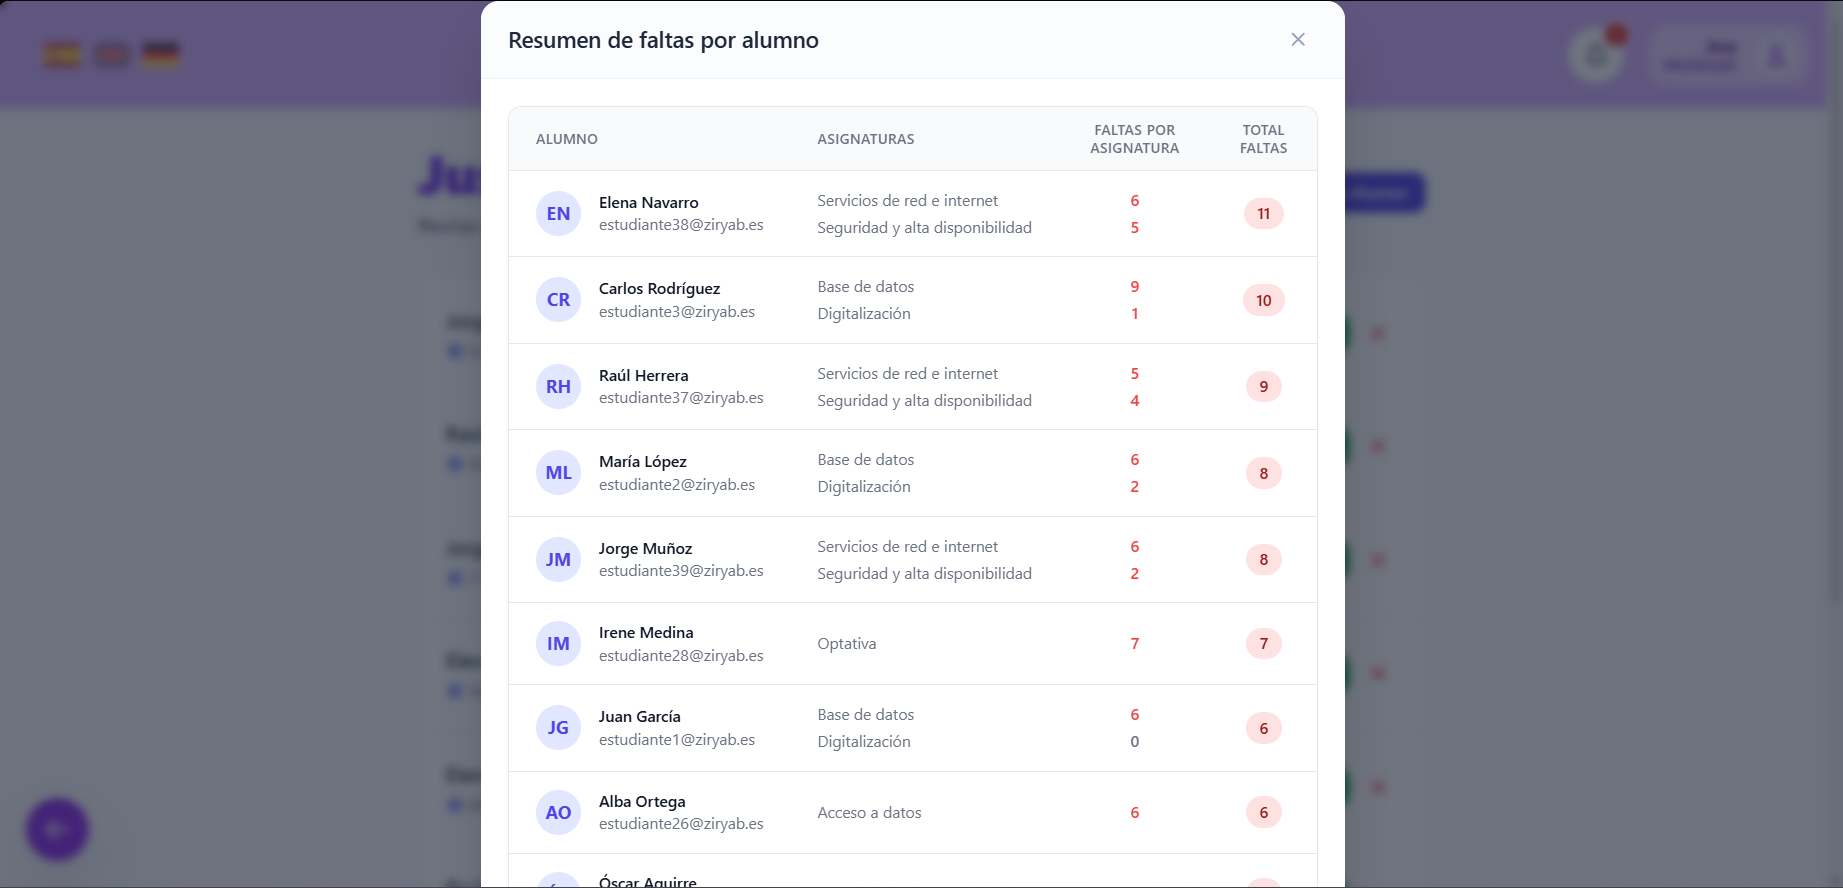
\includegraphics[keepaspectratio,alt={CAPTURA 21 --- Modal de faltas por alumno}]{../../assets/screenshots/manual-profesor/captura21-faltas_por_alumno.png}}
\caption{CAPTURA 21 --- Modal de faltas por alumno}
\end{figure}

\begin{center}\rule{0.5\linewidth}{0.5pt}\end{center}

\section{13. Gestión académica (área
común)}\label{gestiuxf3n-acaduxe9mica-uxe1rea-comuxfan}

Ruta: \textbf{Mi Espacio → Gestión} (\texttt{/gestion}).

Las mismas tarjetas que el alumno, con rutas adaptadas al rol:

{\def\LTcaptype{none} % do not increment counter
\begin{longtable}[]{@{}
  >{\raggedright\arraybackslash}p{(\linewidth - 2\tabcolsep) * \real{0.3333}}
  >{\raggedright\arraybackslash}p{(\linewidth - 2\tabcolsep) * \real{0.6667}}@{}}
\toprule\noalign{}
\begin{minipage}[b]{\linewidth}\raggedright
Tarjeta
\end{minipage} & \begin{minipage}[b]{\linewidth}\raggedright
Destino profesor
\end{minipage} \\
\midrule\noalign{}
\endhead
\bottomrule\noalign{}
\endlastfoot
Ficha Usuario & \texttt{/ficha-usuario} (datos personales; según
configuración) \\
Horario & \texttt{/horario-profesor} \\
Calendario & \texttt{/calendario} \\
Tablón & \texttt{/issues} \\
Evaluaciones & \texttt{/evaluaciones} (solo si eres \textbf{tutor} de un
grupo) \\
\end{longtable}
}

\begin{figure}
\centering
\pandocbounded{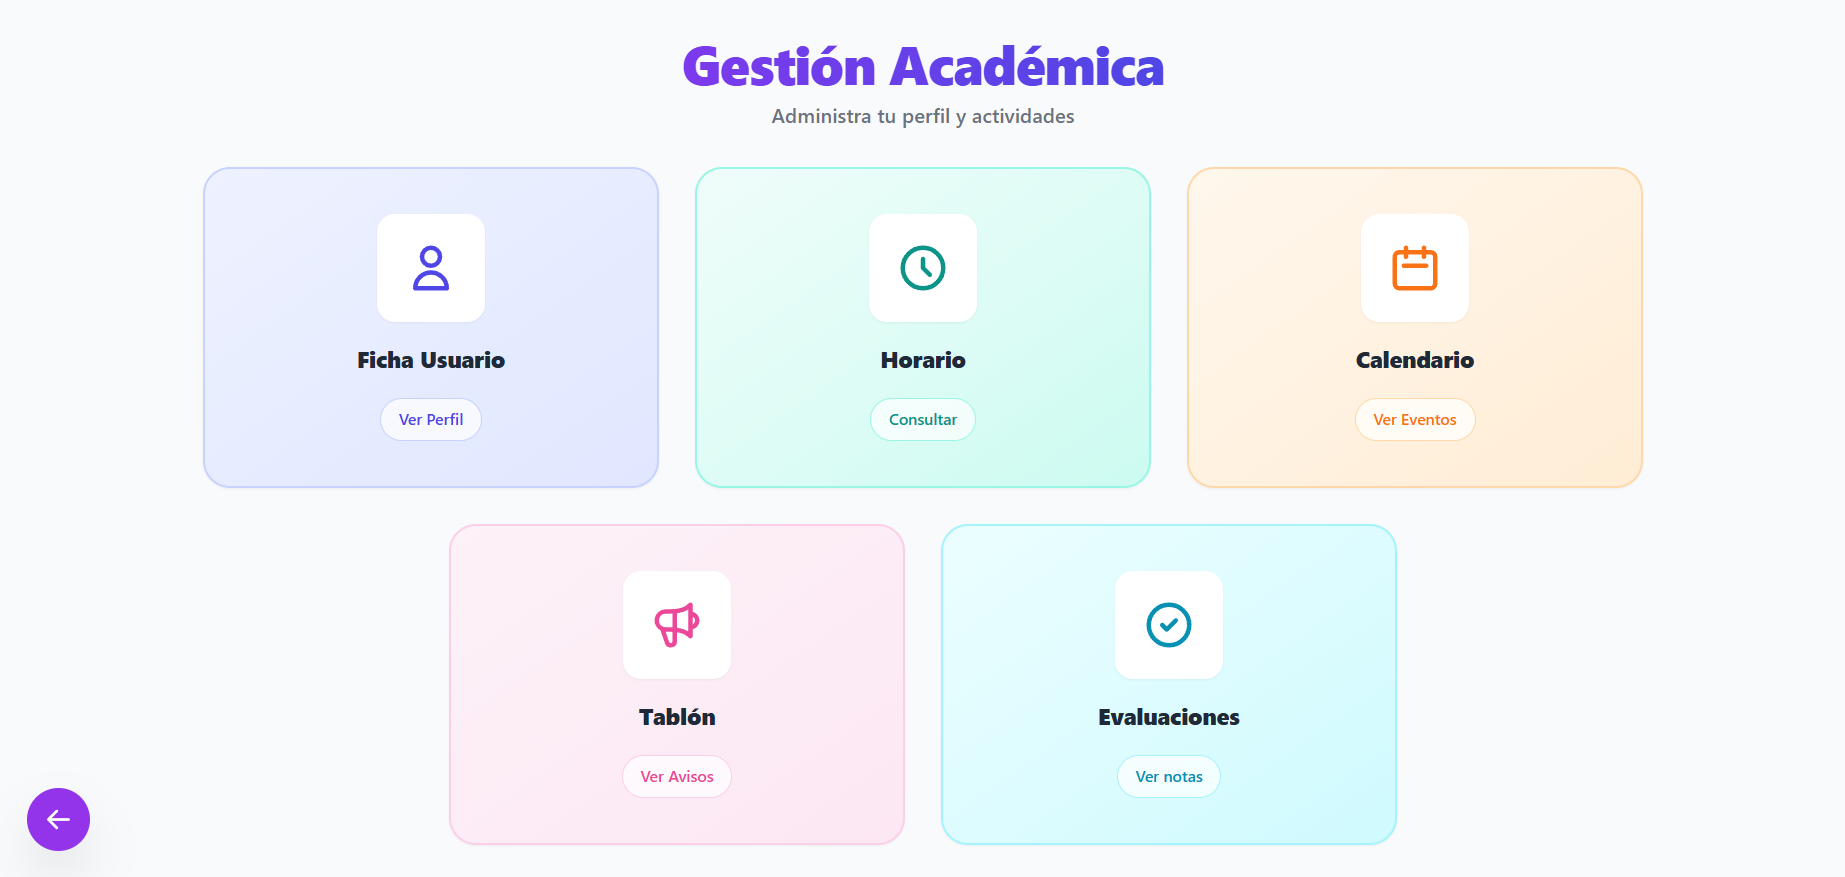
\includegraphics[keepaspectratio,alt={CAPTURA 22 --- Gestión académica vista como profesor}]{../../assets/screenshots/manual-profesor/captura22-gestion.png}}
\caption{CAPTURA 22 --- Gestión académica vista como profesor}
\end{figure}

\begin{center}\rule{0.5\linewidth}{0.5pt}\end{center}

\section{14. Horario del profesor}\label{horario-del-profesor}

Ruta: \textbf{Gestión → Horario} (\texttt{/horario-profesor}).

\begin{itemize}
\tightlist
\item
  Cuadrícula semanal con tus \textbf{franjas de clase} asignadas.
\item
  Cada celda indica hora y asignatura/grupo.
\end{itemize}

\begin{figure}
\centering
\pandocbounded{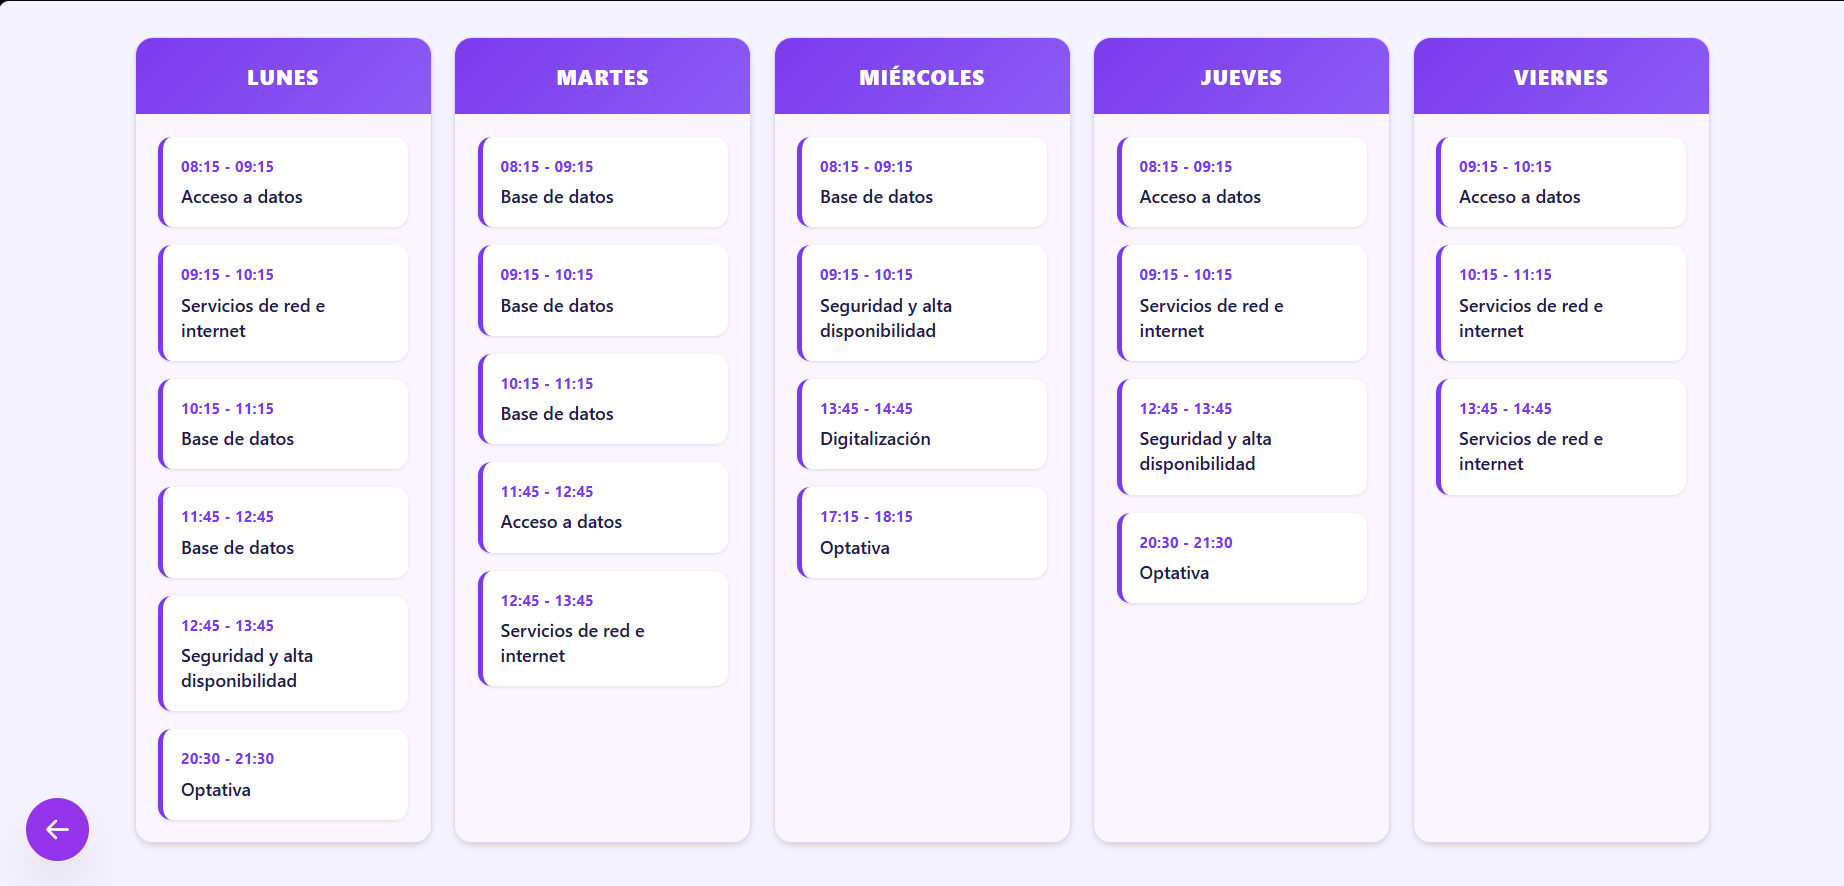
\includegraphics[keepaspectratio,alt={CAPTURA 23 --- Horario semanal del profesor}]{../../assets/screenshots/manual-profesor/captura23-horario.png}}
\caption{CAPTURA 23 --- Horario semanal del profesor}
\end{figure}

\begin{center}\rule{0.5\linewidth}{0.5pt}\end{center}

\section{15. Calendario y tablón}\label{calendario-y-tabluxf3n}

\begin{itemize}
\tightlist
\item
  \textbf{Calendario:} iframe con el calendario institucional
  (\texttt{/calendario}).
\item
  \textbf{Tablón:} anuncios publicados para toda la comunidad
  (\texttt{/issues}).
\end{itemize}

\begin{figure}
\centering
\pandocbounded{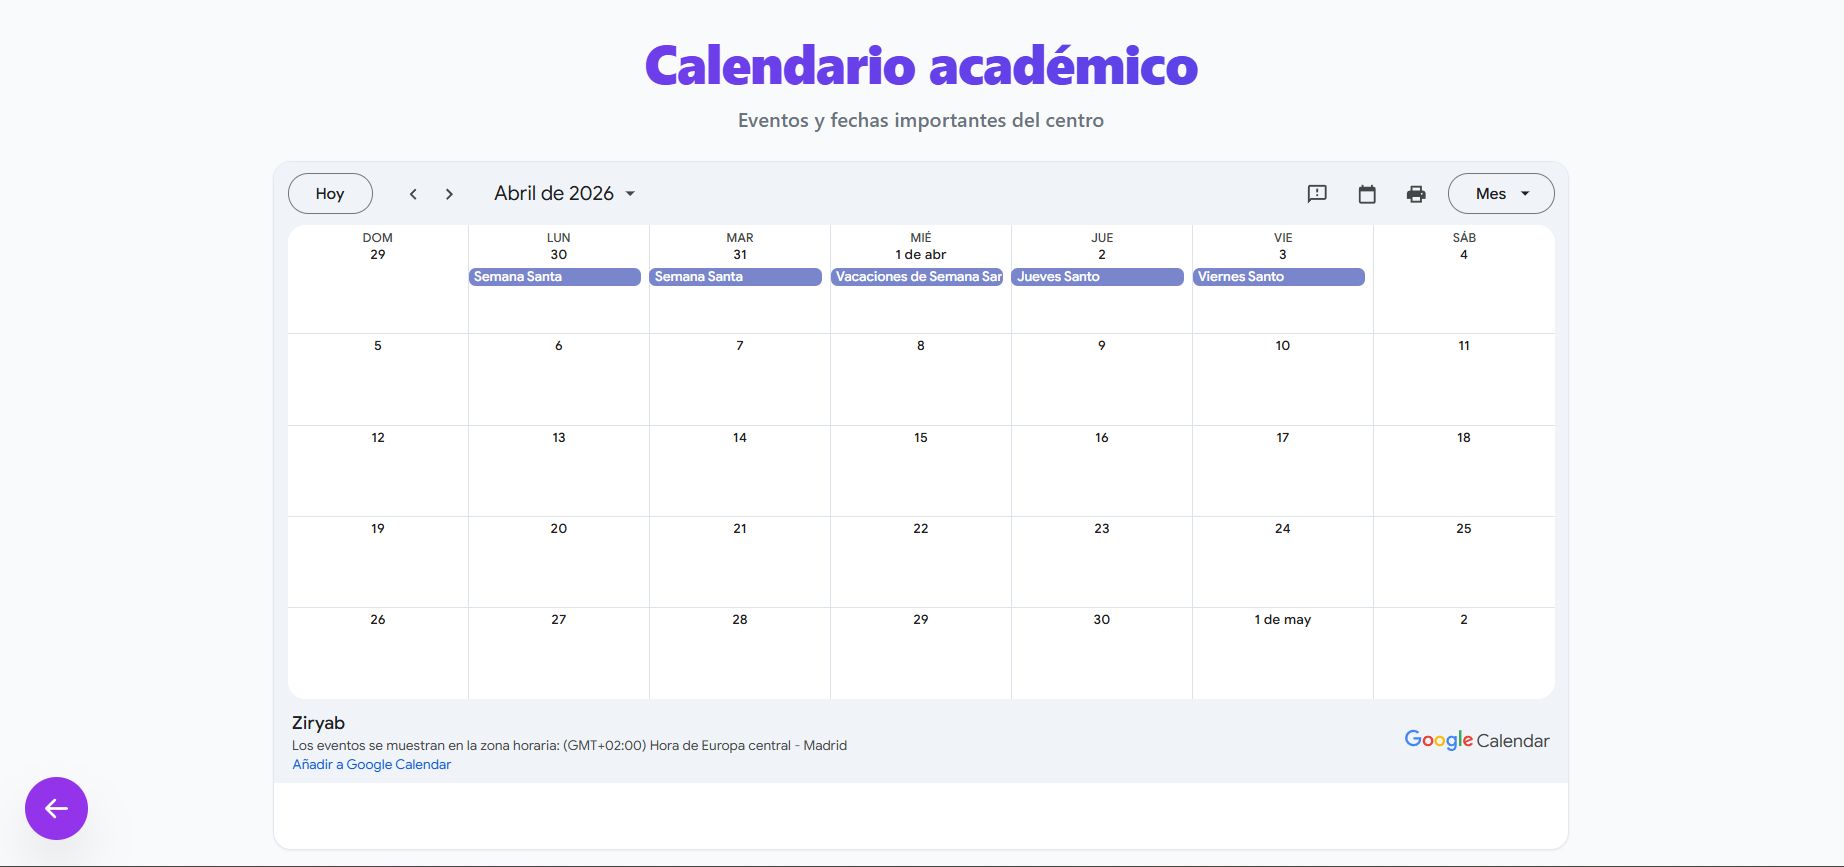
\includegraphics[keepaspectratio,alt={CAPTURA 24 --- Calendario embebido}]{../../assets/screenshots/manual-profesor/captura24-calendario.png}}
\caption{CAPTURA 24 --- Calendario embebido}
\end{figure}

\begin{figure}
\centering
\pandocbounded{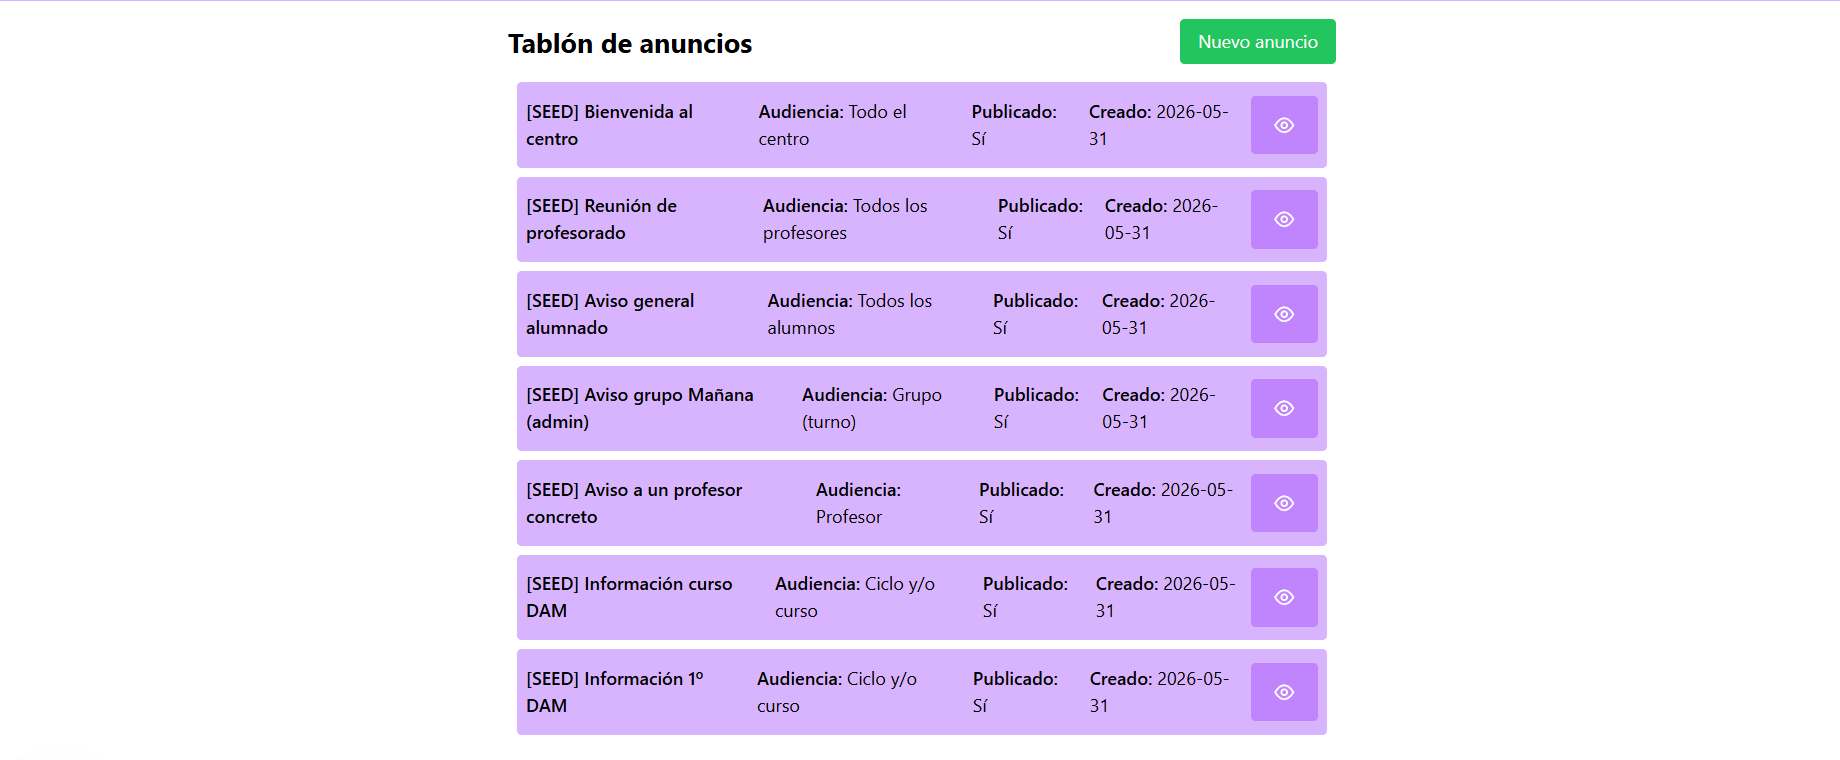
\includegraphics[keepaspectratio,alt={CAPTURA 25 --- Tablón de anuncios}]{../../assets/screenshots/manual-profesor/captura25-tablon.png}}
\caption{CAPTURA 25 --- Tablón de anuncios}
\end{figure}

\subsection{15.1 Crear un anuncio en el
tablón}\label{crear-un-anuncio-en-el-tabluxf3n}

\begin{enumerate}
\def\labelenumi{\arabic{enumi}.}
\tightlist
\item
  Accede al \textbf{Tablón} desde Gestión.
\item
  Pulsa la opción para \textbf{crear un nuevo anuncio} (si tu rol lo
  permite).
\item
  Rellena título y contenido del aviso.
\item
  Publica el anuncio; quedará visible para la comunidad educativa.
\end{enumerate}

\begin{figure}
\centering
\pandocbounded{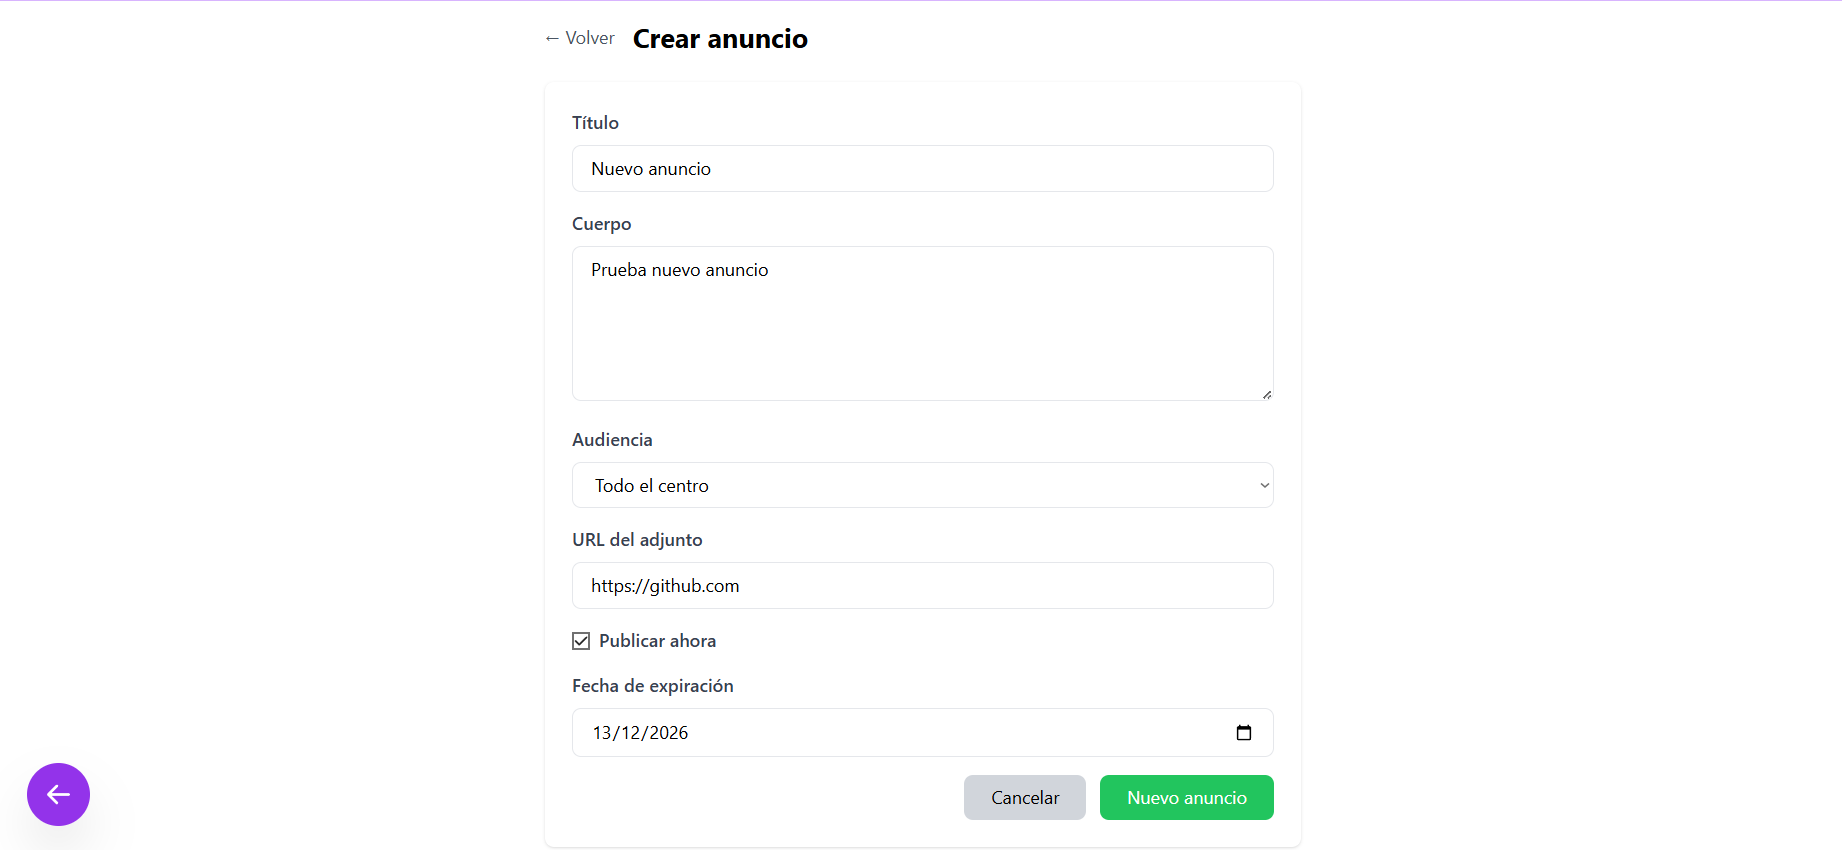
\includegraphics[keepaspectratio,alt={CAPTURA 25.2 --- Formulario crear anuncio}]{../../assets/screenshots/manual-profesor/captura25_2-crear_anuncio.png}}
\caption{CAPTURA 25.2 --- Formulario crear anuncio}
\end{figure}

\begin{center}\rule{0.5\linewidth}{0.5pt}\end{center}

\section{16. Evaluaciones (rol de
tutor)}\label{evaluaciones-rol-de-tutor}

Ruta: \textbf{Gestión → Evaluaciones} (\texttt{/evaluaciones}).

\textbf{Solo disponible si el sistema te tiene registrado como tutor de
un grupo.}

\subsection{16.1 Pantalla principal}\label{pantalla-principal}

\begin{itemize}
\tightlist
\item
  Selector de \textbf{grupo tutorizado} (si hubiera más de uno).
\item
  Selector de \textbf{periodo de evaluación} (inicial, trimestres,
  final).
\item
  Tabla: filas = alumnos del grupo; columnas = asignaturas; celdas =
  notas (1--10).
\item
  Fila o indicador de \textbf{media} por alumno/asignatura.
\end{itemize}

\begin{quote}
\textbf{📷 CAPTURA 26 --- Pantalla Evaluaciones con tabla de notas del
grupo}
\end{quote}

\subsection{16.2 Introducir y guardar
notas}\label{introducir-y-guardar-notas}

\begin{enumerate}
\def\labelenumi{\arabic{enumi}.}
\tightlist
\item
  Selecciona el \textbf{periodo} correcto.
\item
  Rellena todas las celdas obligatorias con notas entre \textbf{1 y 10}.
\item
  Pulsa \textbf{Guardar evaluaciones}.
\item
  Espera el mensaje de éxito.
\end{enumerate}

\textbf{Importante:} El sistema puede exigir que \textbf{todas} las
asignaturas de \textbf{todos} los alumnos tengan nota antes de guardar.

\begin{quote}
\textbf{📷 CAPTURA 27 --- Mensaje de notas guardadas correctamente}
\end{quote}

\subsection{16.3 Sin grupo tutorizado}\label{sin-grupo-tutorizado}

Si no eres tutor, verás: \emph{«No se ha encontrado ningún grupo del que
seas tutor»}.

\begin{center}\rule{0.5\linewidth}{0.5pt}\end{center}

\section{17. Flujos de trabajo
recomendados}\label{flujos-de-trabajo-recomendados}

\subsection{17.1 Publicar una tarea y
calificarla}\label{publicar-una-tarea-y-calificarla}

\begin{Shaded}
\begin{Highlighting}[]
\NormalTok{Mis clases → Gestionar temario → (o Menú de clase → Tareas) → Crear tarea}
\NormalTok{→ Alumnos entregan → Ver entregas → Calificar → Alumno ve la nota}
\end{Highlighting}
\end{Shaded}

\subsection{17.2 Sesión de clase con
asistencia}\label{sesiuxf3n-de-clase-con-asistencia}

\begin{Shaded}
\begin{Highlighting}[]
\NormalTok{Mis clases → Gestionar temario → Pasar lista → Guardar asistencia}
\end{Highlighting}
\end{Shaded}

\subsection{17.3 Revisar una ausencia
justificada}\label{revisar-una-ausencia-justificada}

\begin{Shaded}
\begin{Highlighting}[]
\NormalTok{Menú de clase → Justificaciones → Ver archivo → Aceptar o Rechazar}
\end{Highlighting}
\end{Shaded}

\begin{center}\rule{0.5\linewidth}{0.5pt}\end{center}

\section{18. Preguntas frecuentes
(FAQ)}\label{preguntas-frecuentes-faq-1}

\textbf{¿Por qué no veo Evaluaciones en Gestión?}\\
Esa pantalla es solo para profesores \textbf{tutores}. La asignación la
realiza administración.

\textbf{Un alumno dice que no puede entregar}\\
Comprueba la \textbf{fecha límite} y si la tarea permite \textbf{entrega
tardía}. Revisa en el detalle de la tarea.

\textbf{¿Puedo cambiar una nota ya guardada?}\\
Sí; vuelve a \textbf{Ver entregas → Editar nota} en la entrega del
alumno.

\textbf{El archivo adjunto de creación de tarea falla}\\
Máximo 10 MB; usa formatos permitidos (PDF, DOCX, ZIP, imágenes).

\textbf{No aparecen alumnos al pasar lista}\\
Verifica que haya \textbf{matriculaciones} activas en esa
asignatura-grupo.

\begin{center}\rule{0.5\linewidth}{0.5pt}\end{center}

\section{19. Glosario docente}\label{glosario-docente}

{\def\LTcaptype{none} % do not increment counter
\begin{longtable}[]{@{}
  >{\raggedright\arraybackslash}p{(\linewidth - 2\tabcolsep) * \real{0.4286}}
  >{\raggedright\arraybackslash}p{(\linewidth - 2\tabcolsep) * \real{0.5714}}@{}}
\toprule\noalign{}
\begin{minipage}[b]{\linewidth}\raggedright
Término
\end{minipage} & \begin{minipage}[b]{\linewidth}\raggedright
Definición
\end{minipage} \\
\midrule\noalign{}
\endhead
\bottomrule\noalign{}
\endlastfoot
Asignación & Relación profesor--asignatura--grupo en el sistema \\
Entrega (student-task) & Trabajo enviado por un alumno para una tarea \\
Tutor & Profesor responsable de las notas trimestrales del grupo \\
Justificante & Documento del alumno para excusar una falta \\
LATE & Entrega realizada después del plazo pero permitida \\
\end{longtable}
}

\begin{center}\rule{0.5\linewidth}{0.5pt}\end{center}

\section{20. Resumen de rutas (referencia
rápida)}\label{resumen-de-rutas-referencia-ruxe1pida}

{\def\LTcaptype{none} % do not increment counter
\begin{longtable}[]{@{}ll@{}}
\toprule\noalign{}
Pantalla & Ruta \\
\midrule\noalign{}
\endhead
\bottomrule\noalign{}
\endlastfoot
Login & \texttt{/login} \\
Dashboard & \texttt{/dashboard} \\
Mis clases & \texttt{/clases-profesor} \\
Temario & \texttt{/temario-profesor/:claseId} \\
Menú de clase & \texttt{/menu-clase/:idTeacherAssignment} \\
Tareas & \texttt{/tareas/:idTeacherAssignment} \\
Entregas & \texttt{/tarea/:taskId/entregas} \\
Calificar & \texttt{/calificar-tarea/:id} \\
Justificaciones & \texttt{/ficha-profesor} \\
Gestión & \texttt{/gestion} \\
Horario & \texttt{/horario-profesor} \\
Evaluaciones (tutor) & \texttt{/evaluaciones} \\
\end{longtable}
}

\begin{center}\rule{0.5\linewidth}{0.5pt}\end{center}

\emph{Fin del manual de profesor. Para configuración de grupos,
matrículas o asignación de tutorías, contacta con el rol de
administración del centro.}

\end{document}
